\documentclass[twoside]{projektInzynierskiMS}
\usepackage{polski}
\usepackage[utf8]{inputenc}
\usepackage[intlimits]{amsmath}
\usepackage{caption}
\usepackage{graphicx}
\usepackage{chngcntr}
\usepackage{hyperref}
\usepackage[hyphenbreaks]{breakurl}
\PassOptionsToPackage{hyphens}{url}\usepackage{hyperref}
\graphicspath{ {./images/} }
\numberwithin{figure}{section}
\counterwithout{footnote}{section}
\setcounter{tocdepth}{4}
\setcounter{secnumdepth}{4}
\def\UrlBreaks{\do\/\do-}
\DeclareCaptionType{equ}[Wzór][]
\usepackage{listings}
%\renewcommand{\figurename}{Na rys.}
%\captionsetup[equ]{labelformat=empty}
% Zmiana Listening X na co innego
% \renewcommand{\lstlistingname}{TEST}
\lstset{
    literate={ó}{{\'o}}1 {ż}{{\.z}}1
}

%% tytuł promotor iautor (\title to komenda standardowa)
\title{Implementacja i rozwój wieloplatformowych aplikacji na przykładzie aplikacji wspomagającej system rekrutacji}
\promotor{dr inż. Adrian Kapczyński}


%% każdy autor musi mieć 4 argumenty: imię nazwisko, nr albumu, procent wkładu, opis wkładu
\autor{Dawid Bitner}{275250}{33,33} 
{Rozwój aplikacji od strony aplikacji przeglądarkowej (część kliencka).

Wspomaganie budowy zaplecza systemu aplikacji, implementacja zabezpieczeń (część serwerowa).}
	
\autor{Daniel Broczkowski}{275254}{33,33}
{Rozwój oraz nadzorowanie prac projektu od strony aplikacji przeglądarkowej (część
kliencka).

Wspomaganie budowy zaplecza systemu aplikacji (część serwerowa).}

\autor{Mateusz Kowol}{275282}{33,33}	
{Rozwój oraz nadzorowanie prac projektu od strony aplikacji mobilnej (część kliencka).

Wspomaganie budowy zaplecza systemu aplikacji (część serwerowa).}
	
	

%% dedykacja mile widziana
\dedykacja{Wszystkim ludziom branży IT i nie tylko,\linebreak którzy oferują swoją bezinteresowną pomoc w sieci\linebreak oraz społeczności open source.}
%\NumeryNaPoczatku
%% numeracja wzorów tu włączona typu (1.2.3), ta druga to typu (1.2), domyślnie typu (1)
%\subsectionWzory
% \sectionWzory  

%\rozdzialy


%\literowaNumeracjaDodatkow %% włączy numerację dodatków literami
%\rzymskaNumeracjaDodatkow  %%włączy numerację dodatków liczbami rzymskimi

%% wyłączenie wyjaśnień:
\bezWyjasnien

%% standardowe komendy \newtheorem  działają jak w oryginale
\newtheorem{tw}{Twierdzenie}%[subsection]
\newtheorem{twa}{Twierdzenie}%[section]
\newtheorem{dd}{Definicja}%[subsection]

\begin{document}
\section{Wstęp}

Jednym z wymogów ukończenia studiów przez zespół projektowy było odbycie trzymiesięcznej praktyki zawodowej. W związku z tym członkowie grupy odbyli wiele rozmów kwalifikacyjnych i na ich podstawie nabyli pewne doświadczenia. Jako że sam okres stażu na studiach wiąże się z pisaniem pracy inżynierskiej, pomysł na aplikację wspierającą system rekrutacyjny, zasugerowany przez promotora pracy dyplomowej, idealnie trafił w warsztat umiejętności, jak i gusta zespołu. 

\subsection{Motywacja do wyboru tematu}
Główną motywacją do stworzenia serwisu była zauważalna luka na rynku oprogramowania rekrutacyjnego. Nieznaczna liczba aplikacji umożliwia bezpośrednie przypisywanie testów dla poszczególnych użytkowników, stąd też decyzja o obraniu takiego kierunku. Dzięki temu, że kody są unikalne, istnieje teoretyczna możliwość stworzenia niepowtarzalnych testów bądź różniących się od siebie w taki sposób,\linebreak by wykluczyć możliwość „ściągania” odpowiedzi od innych użytkowników, którzy przystąpili wcześniej do podobnego testu. Daje to szansę indywidualnego podejścia do każdego kandydata. Dodatkowym celem projektu, było przedstawienie zwinnego rozwoju oprogramowania, z wykorzystaniem znanych narzędzi, wspomagających ten proces. Projekt jest swoistą laboratoryjną symulacją rozwoju aplikacji w warunkach komercyjnych. Posiada wymagany temat, termin, podział na role, zarządzanie projektem, kontrolę wersji oraz podział na rozgałęzienia projektu\linebreak w repozytorium.

\subsection{Cel pracy}

Celem pracy inżynierskiej jest opracowanie założeń oraz implementacja z wykorzystaniem znanych wzorców, bibliotek i języków programowania, wieloplatformowego rozwiązania informatycznego wspomagającego rekrutację. Projekt przedstawia informacje o sposobie budowania systemu informatycznego, który z założenia powinien być skalowalny i modularny, aby poszczególne zespoły programistyczne mogły pracować nad rozwojem aplikacji w sposób równoległy, co posiada odwzorowanie\linebreak w projektach komercyjnych.



\subsection{Wspomaganie rekrutacji poprzez systemy informatyczne}
Ostatnie lata przyniosły wiele zmian w procesach rekrutacyjnych, zarówno na stanowiska najniższego szczebla, jak i kierownicze. Dla zwiększenia wydajności, kolejne przedsiębiorstwa starają się usprawnić przebieg zatrudnienia potencjalnych kandydatów, stosując coraz to nowsze sposoby wyboru przyszłych pracowników.\linebreak W tym przypadku, bardzo dużą popularnością cieszy się Internet, za pośrednictwem którego przeprowadzane są wstępne wybory kandydatur, rozmowy rekrutacyjne, czy nawet końcowe etapy rekrutacji, wraz z zawarciem umowy o pracę.

Wiele podmiotów gospodarczych posiada swoje predefiniowane platformy do prowadzenia i rejestrowania przebiegu rekrutacji nowych pracobiorców – co z punktu widzenia kandydata może być kwestią uciążliwą, ponieważ często takie rozwiązania dla danej firmy wymagają założenia w niej konta. Biorąc pod uwagę fakt, że osoba poszukująca pracy zazwyczaj nie aplikuje na stanowisko do jednego konkretnego zakładu pracy, a na ogół robi to mniej lub bardziej masowo, to zagadnienie staje się bardziej problematyczne\footnote{P. Zdziech, „«Nie kupuj Pan cegły», czyli dla kogo platforma do rekrutacji”, \newline \url{https://erecruiter.pl/blog/dla-kogo-platforma-do-rekrutacji/}, (dostęp 21.11.2020)}.
W każdym z systemów potencjalnego pracodawcy, należy posiadać osobny profil, a co za tym idzie -- hasło, które – ze względów bezpieczeństwa – powinno być unikalne w każdym z serwisów. Ma to na celu uchronić nas przed włamaniami do innych platform, gdzie używamy współdzielonych\footnote{W. Earp, „Why sharing passwords is a bad idea”, \newline 
\url{https://swgfl.org.uk/magazine/why-sharing-passwords-is-a-bad-idea/},\newline (dostęp 21.11.2020)}
\footnote{Materiały firmy SolarWinds, „Top Seven Reasons Why You Should Not Share Your Passwords”, \newline 
\url{https://logicalread.com/top-seven-reasons-why-you-should-not-share-your-passwords}, (dostęp 21.11.2020)}
\footnote{Materiały firmy SUNY Broome, „Top reasons why you shouldn’t share your username and password”, \newline \url{https://news.sunybroome.edu/focus/top-reasons-why-you-shouldnt-share-your-username-and-password/}, (dostęp 21.11.2020)} danych logowania. Nieautoryzowane przejęcie konta przez osoby trzecie, grozi wyciekiem większej ilości danych osobowych, za których wykorzystaniem stoją najczęściej nieuczciwe intencje.

Dodatkowo hasło należy odpowiednio zabezpieczyć, co oznacza, że nie powinno składać się ze słów dostępnych w słowniku, naszych danych personalnych, dat urodzenia członków rodziny itp. Takie elementy narażają użytkownika na włamanie do konta np. poprzez socjotechniki bądź znajomość naszej osoby. W powszechnie uznanych zasadach, przyjmuje się, że silne hasło powinno składać się z niezrozumiałego dla osób trzecich ciągu znaków, cyfr, symboli specjalnych oraz powinno uwzględniać wielkie i małe litery – zabezpiecza to użytkownika przed włamaniami z wykorzystaniem metod słownikowych. Kod dostępu nie powinien być zbyt krótki – najlepiej, aby posiadał minimum 8 znaków. Minimalizuje to możliwość jego złamania poprzez ataki typu \textit{brute force}. Dobrą praktyką jest również korzystanie z generatorów haseł, należy jednak upewnić się, że wygenerowane hasło nie zostaje zapisane na serwerach – co otwiera włamywaczowi furtkę do ataku metodą słownikową\footnote{Materiały Massachusetts Institute of Technology, „Strong Passwords”, \newline 
\url{http://kb.mit.edu/confluence/display/istcontrib/Strong+Passwords}, (dostęp 21.11.2020)}
\footnote{Materiały spółki CIS\textsuperscript{\textregistered}, „Do Not Share Your Password”, \newline 
\url{https://www.cisecurity.org/daily-tip/do-not-share-your-password/}, (dostęp 21.11.2020)}. \newline
Przykładowe hasło, niespełniające wymagań bezpieczeństwa:
\begin{center}
    \begin{quote}
        Gliwice123!
    \end{quote}
\end{center}
Przykładowe hasło, spełniające wymogi bezpieczeństwa:
\begin{center}
    \begin{quote}
        \$GEFjx8oa\$i\*
    \end{quote}
\end{center}

\subsubsection{Istniejące rozwiązania na rynku}
\begin{description}
  \item[JOBVITE] -- jest platformą rekrutacyjną w postaci oprogramowania jako usługi (ang. \textit{software as a service, w skrócie SaaS}). Serwis internetowy umożliwia klientom tworzenie zaproszeń do pracy, skierowanych do współpracowników i pracowników, w celu złożenia im przykładowo: propozycji awansu. \textit{Jobvite} integruje się również z serwisami społecznościowymi, takimi jak \textit{Facebook}\linebreak lub \textit{LinkedIn}. Dzięki temu jest korzystnym dostawcą rekrutacji społecznościowej dla firm, z możliwością publikowania ofert pracy i zarządzania procesem rekrutacji. Wśród klientów platformy możemy znaleźć takie podmioty jak \textit{Schneider Electric}, czy \textit{Gamesys}. System daje możliwość przeglądania statystyk, które  dotyczą np. kliknięć w wysłane zaproszenia, jak również gromadzi informacje o kandydatach. \newline
  Więcej informacji: \url{https://www.jobvite.com/}
  \item[Recruitee] -- oprogramowanie, które działa jako system śledzenia kandydatów na poszczególne stanowiska. Obejmuje system edycji witryn karier dla marki pracodawcy, wtyczkę do pozyskiwania personelu, integrację ze stroną internetową, która dotyczy zatrudnienia; synchronizację poczty elektronicznej i kalendarza. Obecnymi klientami są m.in.: \textit{Vice}, \textit{Usabilla} i \textit{Vlisco}. Pracownicy działów zarządzania zasobami ludzkimi mogą dostosować proces rekrutacji na każdą posadę. Użytkownicy mają możliwość przeciągania i upuszczania profili kandydatów na różnych etapach rekrutacji, za pomocą systemu przeciągnij i upuść (ang. \textit{drag and drop}) – takie rozwiązania możemy zauważyć w systemie zarządzania projektem \textit{Jira}, w postaci tablicy \textit{Agile}, która umożliwia zarządzanie przepływem pracy w projektach np.: programistycznych. \newline
  Więcej informacji: \url{https://recruitee.com/}
  \item[Accenture Careers] -- wewnętrzny system korporacji \textit{Accenture}, który wykorzystywany jest do procesów rekrutacyjnych w tymże przedsiębiorstwie. System umożliwia podgląd obecnego statusu kandydata podczas naboru, jak również informacje o terminach i etapach związanych z rekrutacją. \newline
  Więcej informacji: \url{https://www.accenture.com/pl-pl/careers}
\end{description}

\subsubsection{Rozwiązanie zaproponowane w projekcie inżynierskim}
Aplikacja, zrealizowana dla potrzeb projektu inżynierskiegio, umożliwia rejestrację użytkowników, nadawanie im uprawnień dyrektora generalnego firmy (\textit{CEO User}), uprawnień pracowników działów zarządzania zasobami ludzkimi (\textit{HR User}). Członkowie działów HR posiadają uprawnienia, by tworzyć nowe ogłoszenia oraz testy, na które z kolei kandydaci, ubiegający się o pożądane stanowisko, mogą aplikować. Po pozytywnym rozpatrzeniu profilu kandydata na podstawie jego danych\linebreak z życiorysu (łac. \textit{curriculum vitae}), rekruter może przypisać użytkownikowi test, który może rozwiązać. Informacje o nowych zgłoszeniach do testu, jak i o nowych przypisanych testach, są przekazywane użytkownikom działu HR i kandydatom\linebreak w formie mailowej, jak również w postaci powiadomienia na stronie internetowej. Serwis wszystkie swoje możliwości oferuje w części webowej. Aplikacja mobilna oferuje zaś podstawowe funkcjonalności, takie jak: rozwiązywanie testów rekrutacyjnych, obsługę konta i ogłoszeń pracy.

\subsection{Pomysł na rozwiązanie problemu}
W celu realizacji postawionego zadania, wykorzystane zostały popularne środowiska, biblioteki oraz języki predefiniowane do rozwiązań serwerowych i aplikacyjnych od strony serwisu mobilnego i przeglądarkowego.

W realizacji zadania wykorzystana została baza danych \textit{PostgreSQL}, której to przewagą nad konkurencyjnym rozwiązaniem w postaci \textit{MySQL} jest ustawienie indeksowania, które pozwala na wyraźnie szybsze oraz bardziej wydajne przeszukiwanie bazy, która wraz z rozwojem aplikacji, zaczyna nabierać rozmiarów i posiada coraz to więcej rekordów. Warto również zaznaczyć, że bazy \textit{MySQL} w najnowszych wersjach nie są do końca zgodne ze standardem \textit{SQL}. \textit{PostgreSQL} oferuje wysokie prędkości odczytu oraz zapisu, dzięki czemu bardzo dobrze nadaje się do dużych, rozrastających się i skomplikowanych baz danych. \textit{PostgreSQL} to obiektowo-relacyjna baza danych, w której można korzystać z takich abstrakcji, jak dziedziczenie, czy przeciążenie funkcji. Mogą one okazać się bardzo pomocnymi opcjami w większych bazach\footnote{K. Hristozov, „MySQL vs PostgreSQL -- Choose the Right Database for Your Project”, \newline \url{https://developer.okta.com/blog/2019/07/19/mysql-vs-postgres}, (dostęp 21.11.2020)}.

Serwer obsługiwany jest przez technologię \textit{Java Spring Boot}, która zazwyczaj wykorzystywana jest w dużych, komercyjnych projektach, ponieważ jest szeroko znana, stabilna oraz pozwala na skalowalność aplikacji. W \textit{Springu} istnieje wiele modułów, które są wykorzystywane do pracy z np.: chmurami obliczeniowymi, bazami danych\linebreak i mikroserwisami. Dobrze współpracuje z kontenerami \textit{Tomcat Catalina}, dzięki czemu aplikację można z łatwością przenosić na środowiska produkcyjne\footnote{Materiały spółki VMware, „Spring Framework Documentation” \newline
\url{https://docs.spring.io/spring-framework/docs/5.1.0.RELEASE/spring-framework-reference/}, (dostęp 21.11.2020)}.

W rozwoju aplikacji przeglądarkowej wykorzystana została struktura programistyczna (ang. \textit{framework}) \textit{Angular}, który pozwala na modułową (stworzoną\linebreak z serwisów, modułów, komponentów i fabryk) budowę stosunkowo łatwo skalowalnej aplikacji. Wykorzystywana technologia \textit{Single Page Application} (SPA)\footnote{M. Wojciechowski, „Aplikacje SPA, Angular, TypeScript”,\newline
\url{http://www.cs.put.poznan.pl/mwojciechowski/cdv/ria/Angular.pdf}, (dostęp 21.11.2020)} pozwala na przeładowywanie elementów strony, bez jej całkowitego przebudowania, co daje poczucie poruszania się jak po aplikacji desktopowej. Przykładem takiego rozwiązania może być \textit{Google Gmail} – gdzie po otrzymaniu wiadomości strona nie jest przeładowywana, tylko aktualizowana jest zawartość dwóch komponentów – listy odebranych wiadomości i licznika.
Dodatkową zaletą \textit{Angular} jest pisanie aplikacji w języku \textit{TypeScript}, który jest nadzbiorem języka \textit{JavaScript}. Umożliwia programować obiektowo w prosty sposób, a także zapewnia statyczne typowanie. Każdy kod zapisany w \textit{JavaScript} jest poprawnym programem \textit{TypeScript} – z racji bycia jego podzbiorem\footnote{Materiały firmy Microsoft, „TypeScript Documentation”,\newline
\url{https://www.typescriptlang.org/docs/}, (dostęp 21.11.2020)}.

\begin{figure}[h!]
  \centering
  
\includegraphics[width=\textwidth]{images/gmail_example.JPG}
    \caption{Przykład SPA w Gmail. Źródło: Opracowanie własne.}
    \label{fig:gmail_example}
\end{figure}

Aplikacja mobilna została stworzona z użyciem platformy programistycznej \textit{Flutter}, która korzysta z języka \textit{Dart}. Pozytywną cechą tego rozwiązania jest natywność stworzonej aplikacji. Część kodu można napisać za pomocą odpowiednich metod kanałowych (ang. \textit{channel methods}) np.: w \textit{Kotlinie} lub \textit{Swiftcie} – dzięki czemu aplikacja może doskonale współgrać zarówno z systemem \textit{Android} jak i \textit{iOS}. Poprzez wykorzystanie jednego silnika renderowania, framework tworzy dwie natywne aplikacje na oba środowiska – zaoszczędza to czas programiście, ponieważ wystarczy,\linebreak że stworzy jeden kod. Zaletą jest także tzw. \textit{Hotreload}\footnote{Materiały firmy Google, „Flutter documentation”,\newline
\url{https://flutter.dev/docs}, (dostęp 21.11.2020)}, który umożliwia wprowadzanie zmian w działającej aplikacji bez konieczności jej całkowitego przeładowywania – wystarczy, że zostanie odświeżony zmodyfikowany komponent. Dzięki temu można ujrzeć zmiany w aplikacji już po chwili.


\section{Ogólne informacje dotyczące rekrutacji}
Rekrutacja to główny element procesu zarządzania zasobami ludzkimi, najczęściej o charakterze sformalizowanym. Ma za zadanie zachęcić jak największe grono potencjalnych kandydatów do współpracy z pracodawcą. Rozumiana w ten sposób rekrutacja, prowadzi do selekcji petentów, która jest kolejnym etapem procesu wdrożenia nowych pracowników do firmy. Pracodawcy coraz częściej stosują przeróżne techniki, mające za zadanie odsiać ochotników, niespełniających wymogów, np. poprzez wstępne testy, jeszcze zanim przejdzie się do etapu bezpośredniej rozmowy kwalifikacyjnej, na której to z kolei coraz częściej sprawdzane są kompetencje miękkie kandydatów. Wraz z postępem techniki, przedsiębiorstwa czy też agencje specjalizujące się w przeprowadzaniu procesów rekrutacyjnych, wykorzystują do tego internet i rozmowy telefoniczne. Często podczas takiej konwersacji sprawdzana jest np.: ogólna znajomość języka obcego kandydata. Natomiast internet wykorzystywany jest do przeprowadzania rekrutacji bezpośredniej – aplikacji na konkretne stanowisko, wysłania życiorysu, wypełnienia wstępnych testów kompetencji, czy też sprawdzania znajomości potrzebnych zagadnień\footnote{A. Sulich, „Modele i techniki rekrutacji i selekcji realizowane przez przedsiębiorstwa w województwie dolnośląskim", [w:] Nurty badawcze w zarządzaniu, Wydawnictwo GSP, Zgorzelec 2015}.

Taka forma procesu selekcji jest coraz częściej spotykana. Zdalne techniki przeprowadzania procesów rekrutacyjnych przybrały na znaczeniu w dobie pandemii \textit{COVID-19}, gdzie wiele firm przeszło na rekrutację zdalną kandydatów. Obecnie jest to jedyna, a zarazem najlepsza możliwa opcja, która realnie ogranicza kontakty międzyludzkie i minimalizuje ryzyko zakażeniem wirusem \textit{SARS-CoV-2}\footnote{Materiały firmy Grant Thornton, „Rekrutacja i selekcja nie tylko w czasach SARS-CoV-2 -- Purporowy informator", \newline \url{https://grantthornton.pl/wp-content/uploads/2020/06/Covid-rekrutacja-i-selekcja/\_GrantThornton/\_16062020.pdf}, (dostęp 22.11.2020)}.
Wiąże się to z faktem przejścia przez przedsiębiorstwa w pewnym stopniu, lub często\linebreak w całości (w zależności od możliwości), na tryb pracy zdalnej.

\subsection{Rodzaje rekrutacji}
Biorąc pod uwagę środowisko, w jakim poszukuje się nowych kandydatów, można wyznaczyć dwie główne kategorie:
\begin{itemize}
\item \textbf{rekrutację wewnętrzną} – potencjalnymi kandydatami na stanowisko są obecni pracownicy firmy, czyli objęcie posady poprzez awans,
\item \textbf{rekrutację zewnętrzną} – potencjalnymi kandydatami na stanowisko są osoby spoza firmy.
\end{itemize}

Biorąc zaś pod uwagę rozmiar rynku pracy, w jakim prowadzi się poszukiwania, można także wyznaczyć dwie główne kategorie:
\begin{itemize}
\item \textbf{rekrutację wąską} – jak sama nazwa wskazuje, grono osób poszukiwanych na dane stanowisko jest wąskie. Wynika to z tego, że poszukiwani są eksperci\linebreak w określonej dziedzinie. Nie może to być osoba bez doświadczenia, wymaga się od takiej persony najwyższych standardów, które są w stanie zapewnić jedynie nieliczni,
\item \textbf{rekrutację szeroką} – tutaj grono osób poszukiwanych na dane stanowisko jest szerokie. Zazwyczaj poszukuje się masowo nowych pracowników najniższego szczebla. W tym przypadku często nie wymaga się doświadczenia zawodowego, ani wysokich kompetencji, przez co liczba odbiorców jest stosunkowo duża.
\end{itemize}

\subsection{Etapy rekrutacji}
Na proces rekrutacji składają się najczęściej poniższe etapy\footnote{S. Adam, „Modele i techniki rekrutacji i selekcji realizowane przez przedsiębiorstwa w województwie dolnośląskim", [w:] Nurty badawcze w zarządzaniu., Wydawnictwo GSP, Zgorzelec 2015}: 

\begin{description}
\item[Określenie profilu kandydata na podstawie opisu stanowiska pracy] – jest to proces przygotowywania ogłoszenia oferty pracy. Proces ten uważany jest za bardzo ważny, ponieważ to od niego zależy, jacy kandydaci będą aplikować na oferowane stanowisko. Dlatego przeprowadzany jest bardzo dokładnie, gdyż należy starannie przeanalizować, a następnie jasno określić, kto i o jakich kompetencjach jest potrzebny w organizacji.
\item[Tworzenie i zamieszczanie ogłoszeń o stanowisku] – etap polega na doborze odpowiednich mediów, w zależności od rodzaju rekrutacji (szeroka albo wąska). Ogłoszenie powinno zawierać: opis i zakres wymagań, które są stawiane potencjalnym pracownikom; proponowane formy świadczeń i wynagrodzenie, jakie oferuje pracodawca zatrudnionej osobie.
\item[Tworzenie długiej listy kandydatów] – preselekcja. Spośród otrzymanych aplikacji osób, które odpowiedziały na ogłoszenie i spełniają podstawowe wymagania stawiane kandydatom, odrzuca się ochotników, którzy całkowicie nie nadają się na ogłoszony wolny wakat.
\item[Tworzenie krótkiej listy kandydatów] – selekcja osób, które najpełniej spełniają określone wymagania oferty pracy.
\item[Zastosowanie technik naboru kandydatów wobec wybranych osób] – najczęściej w tym momencie ustala się czas i sposób przeprowadzania rozmowy kwalifikacyjnej. Należy również upewnić się, że dany kandydat nadal jest zainteresowany oferowanym stanowiskiem w organizacji.
\item[Sprawdzenie referencji] – często wieloetapowe. Zdarza się, że wstępna rozmowa kwalifikacyjna jest przeprowadzana z pracownikiem działu zarządzania zasobami ludzkimi, natomiast kolejne z osobami na stanowiskach kierowniczych bądź pracującymi na podobnym stanowisku.
\item[Podjęcie decyzji o zatrudnieniu nowego pracownika] – poinformowanie potencjalnego pracownika o pozytywnym albo negatywnym przejściu procesu rekrutacyjnego.
\item[Negocjacje dotyczące warunków zawarcia stosunku o pracę] – jego formy, wynagrodzenia i innych świadczeń. Najczęściej na dane stanowisko są określane przedziały płacowe. Podczas tego etapu przeprowadzane są również negocjacje konkretnej kwoty z tego zakresu.
\end{description}

\subsection{Techniki i narzędzia rekrutacyjne}
\begin{description}
\item[Rozmowa kwalifikacyjna] (wywiad indywidualny) – właściwy etap, w którym organizacja szukająca pracownika ma bezpośredni kontakt z petentem. Podczas rozmowy kwalifikacyjnej pracodawca ustala, czy kandydat jest odpowiednią osobą na stanowisko oraz jaki dodatni wkład może wnieść do firmy\footnote{L. Kulczycka, „Jak najlepiej zaprezentować się podczas rozmowy kwalifikacyjnej", Wydawnictwo Wolters Kluwer Polska SA, Warszawa 2013}.
\item[Ośrodek oceny] (ang. \textit{Assessment center}) – wielowymiarowy proces oceny kompetencji. Do najczęstszych przykładów wykorzystania należą: selekcja i rekrutacja pracowników (zarówno wewnętrzna, jak i zewnętrzna), audyt personalny, działania rozwojowe, a także planowanie kariery i doradztwo.
\item[Testy wiedzy lub kompetencji] – mogą przybierać przeróżne formy, np. testu jednokrotnego wyboru czy z pytaniami otwartymi. Coraz częściej, we wstępnych etapach rekrutacji, testy kompetencji przeprowadzane są z zastosowaniem metod oceny umiejętności kandydata na odległość.
\item[Testy psychometryczne] – ustandaryzowany i zobiektywizowany pomiar próbki zachowania. Pozwala na zbadanie postępowania osoby badanej w sytuacji testowej, co pozwala wywnioskować, jakie działania podejmie kandydat w sytuacjach pozatestowych. W rekrutacji na stanowiska ryzykowne, tj.: kierowca zawodowy czy pracownik służb mundurowych, takie sprawdziany są spotykane dużo częściej, a wręcz uważane są za pewną normę.
\item[Studium przypadku] – (ang. \textit{case study}) – polega na teoretycznym wykonaniu zadania przez kandydata, najczęściej w określonym czasie. Studium przypadku ma na celu wykazanie, że kandydat posiada umiejętności, o których wspomniał w swoim życiorysie, i że potrafi wykonać je w odpowiednim okresie. Zadania w studium przypadku najczęściej rozpoczynają się od słów: zastosuj, oblicz, przygotuj, narysuj, przeanalizuj itp.
\item[Referencje] – zadaniem rekrutera jest sprawdzenie autentyczności referencji posiadanych przez kandydata. Najczęściej wymagane jest przedłożenie dowodów na swoje umiejętności, w postaci uprawnień, dyplomów ukończonych kursów, czy świadectw pracy. Mają one na celu uwiarygodnić przebieg dotychczasowej kariery.
\item[Wywiady ustrukturyzowane] – polegają na zadawaniu pytań, które wcześniej zostały przygotowane przez rekrutującego pracownika i zostają zadane zgodnie ze wcześniej ustaloną kolejnością. Zaletą takiego typu wywiadu jest to,\linebreak że rekruter otrzyma oczekiwane informacje od kandydata (wywiad prowadzony w luźniejszej konwencji tego nie gwarantuje). Główną wadą wywiadu ustrukturyzowanego jest fakt, że selekcjoner może pominąć istotne kwestie lub nie dowie się o umiejętnościach, które kandydat posiada, a o które nie został zapytany.
\item[Wywiady panelowe]  –  to część rozmowy kwalifikacyjnej, w której kandydat odpowiada na pytania grupy osób, które następnie podejmują decyzję o zatrudnieniu. Zatrudniający menedżerowie korzystają z wywiadów panelowych, aby uzyskać spójny obraz kandydata oraz otrzymać natychmiastową opinię od pozostałych członków zespołu\footnote{J. Conway, R. A. Jako, D. F. DeLong, „A meta-analysis of interrater and internal consistency reliability of selection interviews", Artykuł z „Journal of Applied Psychology", 1995}. Wywiady panelowe zmniejszają ryzyko zatrudniania niewłaściwej osoby. Celem panelu jest podjęcie możliwie najlepszej decyzji o zatrudnieniu, biorąc pod uwagę dostępne informacje o stanowisku\linebreak i kandydatach.
\item[Dyskusje grupowe] – mają na celu konfrontację kandydata z osobami zatrudnionymi na podobnym stanowisku bądź z kierownictwem. Często są częścią wywiadów panelowych.
\end{description}


\subsection{Spojrzenie na problem rekrutacji w tekstach kultury}

Dla wielu osób proces rekrutacji jest bardzo stresującym przeżyciem. Kandydaci chcą wypaść dobrze podczas rozmowy kwalifikacyjnej, przedstawić się z jak najlepszej strony. Pracodawca stara się jak najlepiej zbadać potencjalnego pracownika pod kątem jego mocnych i słabych stron. To wszystko sprawia, że u petenta rośnie niepewność. Może on obawiać się o to, czy jego kompetencje są wystarczające. Ludzie, działając pod wpływem stresu, mogą zapominać podstawowych informacji, związanych ze swoją osobą; dziedziną, w której pracują, czy udzielać błędnych odpowiedzi na pytania, na które tak naprawdę znają odpowiedź. Dodatkowo, poza stresem, sam proces rekrutacyjny może być bardzo długi i składać się z wielu etapów. Osoba, które pracuje na regularnym etacie z pewnością nie miałaby większych trudności z wyżej wymienionymi problemami. Sytuacja może być zgoła odmienna\linebreak w przypadku osoby aktualnie bezrobotnej, która przykładowo nie posiada płynności finansowej, jest uzależniona od rodziny, posiada zaciągnięty kredyt lub osoby, która dopiero co wkracza na rynek pracy\footnote{„Stressful experience, brain, and emotions: Developmental, genetic, and hormonal influences", McEwen (1995)}. Rozmowa kwalifikacyjna jest na pewno stresującą sytuacją w życiu. Na temat przebiegu rekrutacji istnieje wiele mitów, które zostały zobrazowane w różnych tekstach kultury\footnote{„Filmy dla rekrutera", Katarzyna Rojewska \newline
\url{https://nofluffjobs.com/blog/filmy-dla-rekrutera/} (dostęp 23.11.2020)}:

\textbf{Test} – film reżyserii \textit{Stuarta Hazeldine'a} jest opowieścią o ósemce śmiałków, przystępujących do ostatniego etapu rekrutacji w bardzo tajemniczej korporacji. Każdy z kandydatów otrzymuje jedno pytanie oraz trzy reguły, których nie może złamać. Na udzielenie odpowiedzi każdy z ochotników ma nie mniej i nie więcej niż godzinę i dwadzieścia minut. Bohaterom bardzo zależy na wygranej. Powoduje to, że w pewnym momencie przestają nad sobą panować i zaczynają zachowywać się nieludzko, agresywnie. W pewnym momencie sytuacja zaczyna wymykać się spod kontroli i już nie przypomina standardowej rekrutacji. Film w dosadny sposób opisuje tzw. „wyścig szczurów” i pogoń za pieniędzmi, która w obecnych czasach potrafi przyćmić prawdziwy obraz rzeczywistości.

\textbf{Metoda} -- film autorstwa \textit{Marcelo Piñeyro}. Historia przedstawia rywalizację siedmiu kandydatów, ubiegających się o stanowisko międzynarodowego kierownika\linebreak w jednej z korporacji. Wybrany zostanie tylko jeden spośród nich. Każdy z ochotników reprezentuje inny rodzaj osobowości. Atmosfera panująca podczas procesu rekrutacyjnego zaczyna wzbudzać w uczestnikach niepewność i wywołuje paranoję. Grupa poddawana jest serii prób i testów psychologicznych, których zadaniem jest eliminacja i wybór tylko jednego – najlepszego kandydata.

\subsection{Przepisy prawne stosowane podczas rekrutacji}
Proces rekrutacyjny wiąże się z pozyskiwaniem przez potencjalnego pracodawcę danych osobowych, zawartych w dokumentach kandydata, wyrażającego chęć podjęcia zatrudnienia. Należy podkreślić, że pracodawca nie może żądać od petenta danych, które nie są potrzebne do przeprowadzenia rekrutacji, jak np.: stan cywilny, czy orientacja seksualna. Dane osobowe nie mogą być zbierane przez administratora bez powodu zgodnego z prawem, a mogą wyłącznie wtedy, kiedy są niezbędne do realizacji tego celu, jakim jest proces rekrutacji. Podsumowując -- administrator danych osobowych podczas rekrutacji nie może zbierać informacji, które nie są przydatne w procesie rekrutacyjnym\footnote{Rozporządzenie Parlamentu Europejskiego i Rady (UE) 2016/679 z dnia 27 kwietnia 2016 r. w sprawie ochrony osób fizycznych w związku z przetwarzaniem danych osobowych i w sprawie swobodnego przepływu takich danych oraz uchylenia dyrektywy 95/46/WE (ogólne rozporządzenie o ochronie danych)} \footnote{Rozporządzenie Ministra Rodziny, Pracy i Polityki Społecznej z dnia 10 grudnia 2018 r. w sprawie dokumentacji pracowniczej (Dz. U. poz. 2369)}, chyba że kandydat zrobi to dobrowolnie i za specjalnym oświadczeniem – nawet w takiej sytuacji, dodatkowe informacje podane przez kandydata nie mogą wpływać na przebieg rekrutacji (np.: kobieta, nieplanująca posiadania potomstwa, nie może stać na uprzywilejowanej pozycji w stosunku do kandydatki, która ma zamiar w najbliższym czasie zajść w ciążę – pomimo tego, że pracodawca może widzieć w tym korzyści, jak np. dostępność pracownika, czy brak konieczności wypłacania świadczenia podczas urlopu macierzyńskiego). Przyszły pracodawca może jednak żądać przedłożenia dodatkowych, określonych prawem dokumentów czy kwalifikacji, jeśli wynika to z konkretnego charakteru pracy. Takim dokumentem jest np. zaświadczenie o niekaralności -- u kandydata do służb mundurowych czy pracownika sądu, prawa jazdy odpowiedniej kategorii u kierowcy, czy uprawnień do obsługi konkretnej maszyny u operatora.
Przyszły pracodawca nie ma prawa żądać od kandydata informacji o toczących się i niezakończonych postępowaniach karnych oraz o ich obecnym przebiegu. Dane tego typu nie mieszczą się bowiem w katalogu informacji możliwych do przetwarzania w procesie rekrutacji, gdyż pomimo prawnej możliwości żądania informacji o karalności w określonych przypadkach, postępowanie karne nie musi doprowadzić do prawomocnego skazania danej osoby.

Zgodnie z art. 221$^{1}$ § 1 Kodeksu pracy\footnote{Ustawa z dnia 26 czerwca 1974 r.- Kodeks Pracy (Dz. U. z 2019 r. poz. 1040, 1043 i 1495)}, pracodawca może żądać od kandydata do pracy podania danych osobowych, które obejmują poniższe informacje:

\begin{itemize}
\item imię (imiona i nazwisko),
\item datę urodzenia,
\item dane kontaktowe wskazane przez kandydata,
\item wykształcenie,
\item kwalifikacje zawodowe,
\item przebieg dotychczasowego zatrudnienia.
\end{itemize}


Prowadzenie dokumentacji pracowniczej (po zatrudnieniu) odbywa się na podstawie odrębnych przepisów prawa pracy. Rozporządzenie Ministra Rodziny Pracy i Polityki Społecznej z 10 grudnia 2018 r. określa zakres oraz sposób prowadzenia i przechowywania akt pracowników. Nie można zatem mówić o dobrowolności podczas przetwarzania danych o zatrudnionych pracownikach, ponieważ ta kwestia jest regulowana przez powyższe rozporządzenie.

Pracodawca musi mieć na uwadze możliwość wycieku danych osobowych oraz musi stosować środki zapobiegawcze, jak np. przetrzymywanie informacji w systemach elektronicznych o nienagannym poziomie zabezpieczeń i autoryzacji, czy zabezpieczonego fizycznego archiwum. W przypadku wycieku danych, pracodawca musi niezwłocznie (w przeciągu 72 godzin od momentu wykrycia incydentu) poinformować osoby, których dane zostały wykradzione. Dodatkowo musi zgłosić ten fakt do odpowiedniego organu nadzorczego – wskazuje na to Art. 33 RODO. Również na pracowniku, który zauważy wyciek, ciąży powinność niezwłocznego poinformowania o tym pracodawcy.
\newpage

\textbf{Podsumowując, rekrutacja to bardzo trudny i złożony proces, do którego różne przedsiębiorstwa podchodzą w zindywidualizowany sposób, dodatkowo pod uwagę muszą być brane często kwestie prawne, związane zarówno z kodeksem karnym, jak i \textit{RODO}. Sam proces rekrutacji bywa stresującym przeżyciem dla kandydatów, z tego też powodu jest to częsty motyw w przeróżnych tekstach kultury np. produkcjach filmowych. Brak tutaj standardu, który zapewniałby klarowność tego procesu od samego początku. Wieloplatformowa aplikacja, która wspierałaby przeprowadzanie wspomnianego procesu, z pewnością byłaby bardzo przydatna w wielu średnich firmach, jak i korporacjach. Przyczyniłaby się także do redukcji kosztów, związanych z prowadzeniem działalności gospodarczej, poprzez zmniejszenie nakładu czasowego potrzebnego na przeprowadzanie procesu rekrutacji.}


\section{Założenia projektowe}
W rozdziale zostały omówione w zwięzły sposób początkowe założenia, dotyczące realizacji projektu inżynierskiego. Po wstępnej analizie problemu, zostały sporządzone założenia wyjściowe, które dotyczą poszczególnych części serwisu.

\subsection{Wstępne założenia dotyczące serwera i bazy danych}
Podczas rozważania założeń dotyczących części zaplecza aplikacji, zostały wyszczególnione następujące punkty, które projekt powinien spełniać:
\begin{itemize}
\item kod aplikacji powinien działać stabilnie, szybko i sprawnie (najlepiej skorzystać z popularnego i rozwijanego frameworku, co zapewni dodatkowo dużą bazę wsparcia technicznego),
\item odporność na skomplikowane zapytania,
\item szybkość odpowiedzi dla dużych ilości informacji,
\item serwer i baza powinny być łatwe w rozbudowaniu,
\item wsparcie dla wzorców projektowych (np. \textit{Model View Controller}),
\item operacje głównie na obiektach,
\item łatwość konfiguracji,
\item tworzenie tabel i zależności w bazie danych na poziomie kodu programu,
\item wsparcie dla modułów bezpieczeństwa.
\end{itemize}
Na podstawie powyższych wymagań, jako środowisko dla \textit{backendu} zostało wybrane połączenie bazy danych \textit{PostgreSQL} oraz serwera \textit{Spring}. Baza danych \textit{PGSQL} jest uznawana w środowisku programistycznym za najlepsze rozwiązanie od strony baz danych dla aplikacji, która ma potencjał się rozrastać. \textit{Spring} natomiast jest technologią, która na rynku jest od osiemnastu lat i nadal jest rozwijana, posiada wsparcie oraz uznawana jest za bezpieczną.

Następnie zostały wykonane szkice bazy danych, które determinują również budowę aplikacji serwerowej.

Według wstępnych założeń, w bazie danych powinny znaleźć się następujące tabele:

\begin{itemize}
    \item \textbf{account\_types} (rodzaje kont) w relacji jeden do wielu, z tabelą \textit{users},
    \item \textbf{answers} (odpowiedzi) – zawierająca możliwe odpowiedzi na konkretne pytania, w relacji jeden do wielu z tabelą  \textit{questions},
    \item \textbf{ceos} (właściciele firm) – zawierająca informację o właścicielach firm, w relacji jeden do jednego z tabelą \textit{users}, oraz wiele do jednego z tabelą \textit{companies} – jako założyciele,
    \item \textbf{companies} (firmy) – zawierająca informacje o firmach, takie jak np. adres, czy nazwę,
    \item \textbf{company\_pictures} (zdjęcia firmy) – przeznaczona do przetrzymywania informacji o multimediach, dotyczących firmy, takich jak zdjęcia budynku, czy logo. W kolumnie o typie tekstowym, przetrzymywana będzie część odnośnika do serwera \textit{FTP}, w ten sposób większość zawartości bazy danych nie będzie zapełniona przez dane typu \textit{blob}, a w celu fizycznego przetrzymywania plików na dysku, zostanie wykorzystany serwer \textit{FTP},
    \item \textbf{hr\_user} (użytkownicy działu zarządzania zasobami ludzkimi) – powiązania\linebreak z tabelą \textit{companies} w relacji wiele do jednego oraz z tabelą \textit{users} w relacji jeden do jednego,
    \item \textbf{questions} (pytania) – zawierająca treści pytań do poszczególnych testów,\linebreak w relacji wiele do jednego z tabelą \textit{tests},
    \item \textbf{test\_participant} (przypisanie do testu) – zawierająca informacje o przypisanych kodach do testów dla poszczególnych użytkowników, aktualny numer pytania, na którym jest użytkownik, czas rozpoczęcia oraz zakończenia testu. W relacji wiele do jednego z tabelą \textit{tests}, wiele do jednego z tabelą \textit{users},
    \item \textbf{tests} (testy) – zawierająca informacje o poszczególnych testach, utworzonych przez pracowników: czy test jest aktywny, czy jest możliwość cofania pytań,\linebreak w relacji wiele do jeden z tabelą \textit{companies},
    \item \textbf{user\_answers} (odpowiedzi użytkowników) – zapisują się w niej informacje\linebreak  o udzielonych odpowiedziach. W relacji wiele do jednego lub jeden do jednego z tabelą \textit{questions} -- zależne od dalszych ustaleń, wiele do jednego z tabelą \textit{tests} oraz wiele do jednego z tabelą \textit{users},
    \item \textbf{users} (użytkownicy) – zawierająca informacje o zarejestrowanych użytkownikach, hasła użytkowników zaszyfrowane są przez \textit{bcrypt}.
\end{itemize}

Natomiast podstawowe punkty końcowe powinny umożliwiać:
\begin{itemize}
    \item logowanie oraz rejestrację użytkowników,
    \item dodawanie ogłoszeń przez pracowników firmy,
    \item dodawanie pracowników do firmy przez właściciela,
    \item tworzenie oraz rozwiązywanie testów,
    \item tworzenie oraz aplikowanie na ogłoszenia.
\end{itemize}

\subsection{Wstępne założenia dotyczące aplikacji webowej}
Przy omawianiu założeń dotyczących aplikacji, zespół brał pod uwagę takie wymagania, jak:
\begin{itemize}
    \item dostępność źródeł i pomocy dla programisty,
    \item aktualność platformy programistycznej,
    \item modułowość,
    \item responsywność,
    \item możliwość obiektowego tworzenia aplikacji, zagnieżdżania komponentów,
    \item prosta obsługa nagłówków (w tym „doczepianie” informacji o tokenie).
\end{itemize}

W trakcie analizy podjęto decyzję o wyborze środowiska programistycznego \textit{Angular}, który wykorzystuje język \textit{TypeScript}, ponieważ doskonale spełnia on nakreślone wcześniej wymagania. Posiada bardzo przystępny sposób tworzenia komponentów, jest ciągle rozwijany, a także -- dzięki \textit{Node Package Module} -- posiada dostęp do wielu bezpłatnych bibliotek, pomagających rozwijać aplikację. Dodatkowo zespół posiada w nim największe doświadczenie, spośród wszystkich popularnych frameworków frontendowych.

Zespół w trakcie burzy mózgów zdecydował o tym, co powinna oferować aplikacja przeglądarkowa. Do tych wymagań należą:
\begin{itemize}
    \item logowanie i rejestracja użytkowników,
    \item uwierzytelnienie na podstawie tokenu,
    \item rozróżnienie i dostosowanie interfejsu na podstawie rodzaju konta (administrator, zwykły użytkownik, pracownik działu zarządzania zasobami ludzkimi, przedstawiciel firmy),
    \item możliwość przeglądania listy ogłoszeń,
    \item aplikacja przygotowana w minimum dwóch językach (polskim i angielskim),
    \item możliwość tworzenia testów rekrutacyjnych przed pracowników firmy,
    \item możliwość dodania firmy,
    \item możliwość rozwiązywania testów rekrutacyjnych.
\end{itemize}

\subsection{Wstępne założenia dotyczące aplikacji mobilnej}
Zespół postawił na framework \textit{Flutter}, korzystający z języka \textit{Dart}. Czynniki, które o tym zadecydowały, to m.in.: 
\begin{itemize}
    \item tworzenie aplikacji na dwa systemy (\textit{iOS} i \textit{Android}) równolegle,
    \item prostota budowy aplikacji,
    \item technologia o dużym wsparciu społeczności.
\end{itemize}

Aplikacja mobilna jest mniej rozbudowaną wersją tej przygotowanej na przeglądarkę, powinna umożliwiać takie działania jak:
\begin{itemize}
    \item logowanie i rejestracja zwykłego użytkownika,
    \item powiadomienia o przypisanych testach,
    \item możliwość rozwiązywania testu.
\end{itemize}
\textbf{Wszystkie wymienione w tym rozdziale założenia nie są założeniami końcowymi, w trakcie rozwoju aplikacji mogły ulec zmianie – zostać zmodyfikowane, usunięte lub też mogły pojawić się nowe.}

\section{Metodyka}
Rozdział ten przedstawia kolejne trzy fazy realizacji, które zostały wyszczególnione podczas tworzenia projektu inżynierskiego.
\subsection{Faza planowania}
Najważniejszym, a zarazem najbardziej oczywistym punktem, był wybór tematyki pracy. Po ustaleniu tej kwestii, nastąpiła faza planowania. 

Dla łatwiejszego zobrazowania problemu, został sporządzony prosty szablon aplikacji webowej oraz mobilnej. Dzięki temu łatwiej było określić, jakie komponenty należy powołać do życia oraz jakie punkty końcowe trzeba stworzyć do ich obsługi. 
Po spisaniu wstępnych zadań, nastała pora na ich podział pomiędzy członków projektowych oraz śledzenie postępów. Pozostał jeszcze wybór narzędzia do monitorowania efektów. Rozważane były dwie opcje, należące do firmy \textit{Atlassian}. Pierwszym\linebreak z nich było \textit{Trello} – aplikacja online do tworzenia list w stylu \textit{Kanban}. Jest to propozycja sprawdzona przy mniejszych projektach i sprawuje się relatywnie dobrze, jednak przegrała ona z drugim kandydatem – \textit{Jira}. Zarówno jedno, jak i drugie oprogramowanie pozwala na generowanie zadań, dzielenie ich na dowolne sekcje, przypisywanie wykonawców, ustalanie terminów oraz ustawianie statusów przebiegu realizacji. \textit{Trello} nie zostało wybrane przez członków zespołu z kilku przyczyn. Pierwszą\linebreak z nich było to, że darmowa wersja jego rywala posiadała wtyczkę, dzięki której można synchronizować system kontroli wersji \textit{Git} wraz z tablicą. Wystarczy tylko, że nazwy zatwierdzeń zaczynają się od identyfikatora zadania. Wtedy w systemie zapisywane\linebreak są informacje o kolejnych rozgałęzieniach i zatwierdzeniach zmian dla wybranego zadania. Dzięki temu można w prosty sposób sprawdzić z poziomu \textit{Jiry} postęp prac, bez potrzeby manualnego doszukiwania się aktualizacji kodu. Kolejną przyczyną była chęć nauki czegoś, co jest realnie wykorzystywane przy dużych projektach w świecie biznesu. Co za tym idzie, można podnieść zarówno swoje kompetencje, jak i samą pracę inżynierską na wyższy poziom standardów. Ostatecznym punktem, który zadecydował o porażce \textit{Trello}, był fakt, że nie pozwala ono na rejestrowanie czasu poświęconego na realizację zadania. Dzięki tej funkcjonalności można\linebreak z łatwością stwierdzić, które zagadnienia sprawiają najwięcej problemów i gdzie przydałaby się pomoc innego członka projektu.

Ostatnim punktem, a zarazem najbardziej oczywistym, było zaadresowanie kwestii systemu kontroli wersji. Wybór dość szybko padł na platformę \textit{GitHub}, głównie ze względu na jej znajomość i niezawodność. Pomimo tego, że chyba nie ma na świecie programisty, który by choć raz nie skorzystał z tego oprogramowania \linebreak i większość uznaje je za coś oczywistego, to nie można pomniejszać jego roli, którą odegrało w pracy. Rozwiązanie to stanowi swoisty szkielet całego projektu i bez niego nie byłoby szans na ukończenie kodu w zadanym terminie.
\subsection{Wczesna faza implementacji}
Pierwszym implementacyjnym krokiem projektu było powołanie do życia strony serwero–bazodanowej. Następną rzeczą, którą należało zrobić, było przetestowanie stworzonego zaplecza. W tym celu użyto oprogramowanie \textit{Postman}. W skrócie, pozwala ono na generowanie i wysyłanie zapytań do \textit{API} (ang. \textit{application programming interface}) oraz wyświetlanie zwracanych odpowiedzi. Po upewnieniu się,\linebreak że podstawowe punkty końcowe działają, nastała faza implementacji aplikacji internetowej. Połączenie frontendu z backendem nie przysporzyło większych problemów\linebreak i wszystko zadziałało tak, jak powinno. Zostały utworzone podstawowe panele\linebreak i komponenty, które, choć puste, były bardzo ważne, bo to właśnie one uwidaczniały, jak wiele pracy jeszcze przed zespołem. Na tym etapie został utworzony szkielet aplikacji, wokół którego można było budować resztę ciała. Część mobilna dostała niższy priorytet i została przeznaczona na dalsze etapy rozwoju.
\subsection{Zaawansowana faza implementacji}
Mając gotową bazę, pozostało uzupełniać ją o funkcjonalności. W pierwszej kolejności należało obrać za cel konkretny komponent aplikacji. Następnie w pełnym składzie dokładnie przedyskutowano zasadę jego działania. Po omówieniu wszystkich za i przeciw, utworzono odpowiednie punkty końcowe w części serwerowej,\linebreak a następnie obsłużono je po stronie aplikacji internetowej. Jeśli wszystko zadziałało zgodnie z planem, to cały ten proces powtarzany był od nowa, a jeśli nie, to należało dojść do tego, dlaczego założenia się nie sprawdziły i zmienić je na właściwe.
\subsection{Faza stabilizacji}
Faza stabilizacji nastała po tym, gdy wszystkie planowane funkcjonalności zostały oprogramowane. To właśnie wtedy przyszedł czas na wyszukiwanie i zwalczanie wszelkich błędów w kodzie i niepożądanych zachowań aplikacji. Poza szlifowaniem działania serwisu, należało przyjąć wspólne założenia, co do finalnego stylu programu przeglądarkowego i mobilnego. Tak, aby były one w miarę możliwości jednolite, co do szaty graficznej oraz designu.

Poza pracami nad kodem, zostały także rozpoczęte intensywne prace nad dokumentacją, którą -- według ustaleń -- należało skończyć do połowy grudnia. Termin ten został wybrany tak, aby mieć odpowiedni bufor czasowy na wszelkie poprawki i niespodziewane problemy, o których warto byłoby wspomnieć.
\newline

\textbf{Podczas prac nad projektem można było zauważyć i wyróżnić kilka faz, w których projekt się znajdował. Były nimi: 
\begin{itemize}
    \item faza planowania -- podczas której zespół stworzył pierwsze szkice projektu,
    \item wczesna faza implementacji -- gdzie zespół wprowadził podstawowy model bazy danych;
    zaawansowana faza implementacji -- skupiająca się przede wszystkim na funkcjonalnościach części klienckiej i punktach końcowych części serwerowej,
    \item faza stabilizacji -- czyli ostatnie poprawki i testowanie projektu.
\end{itemize}
Podzielenie pracy na tego typu etapy sprawiło, że aplikacja nie była pisana chaotycznie, a każdy z członków zespołu łatwiej odnajdywał się w swoich zadaniach i wiedział, w jakim tempie posuwają się prace\linebreak w perspektywie pozostałego czasu.}

\section{Technologie}
Rozdział ten został poświęcony opisom technologii, które zostały wykorzystane podczas tworzenia projektu inżynierskiego.

\subsection{Serwer i baza danych}
Głównymi technologiami, użytymi w tworzeniu zaplecza serwisu, były m.in. \textit{PostgreSQL} oraz \textit{SpringBoot}.

\subsubsection{PostgreSQL}
Jest to otwarty (ang. \textit{open source}), obiektowo–relacyjny system zarządzania bazami danych. W okresie ponad trzydziestu lat zyskał na reputacji dzięki swojej wydajności, niezawodności, spójności danych i ich poprawności. Poza jego charakterystyką, ważne jest także to, że projekt ten jest rozwijany przez ochotników z całego świata, przez co jest bezpłatny.

Więcej informacji: \url{https://www.postgresql.org/}
\subsubsection{SpringBoot}
Wydajne i proste narzędzie, ułatwiające tworzenie aplikacji opartych o mikroserwisy w \textit{Javie}. Dzięki niemu programiści nie muszą, między innym, zajmować się zachowaniem prawidłowych zależności pomiędzy dodawanymi bibliotekami, przez co unika się problemu niekompatybilności między nimi podczas konfigurowania \textit{API}. Odchodzi również wymóg posiadania zewnętrznego serwera, na który trzeba by było wgrywać aplikację, a później weryfikować jej poprawność. Wszystko to przekłada się na bardziej efektywne pisanie kodu, oszczędność czasu i łatwość obsługi.

Głównymi zaletami \textit{SpringBoota} są:
\begin{itemize}
    \item budowanie samodzielnej aplikacji (ang. \textit{stand-alone application} za pomocą tak zwanych starterów, czyli zbioru wszystkich niezbędnych konfiguracji oraz bibliotek,
    \item brak wymogu konfiguracji \textit{XML} (ang. \textit{Extensible Markup Language}),
    \item wbudowany serwer i inne niezbędne zależności i komponenty, potrzebne do uruchomienia aplikacji.
\end{itemize}

Więcej informacji: \url{https://spring.io/projects/spring-boot}
\subsubsection{Spring Security}
Potężna i wysoce konfigurowalna struktura (ang. \textit{framework}), wykorzystywana do uwierzytelniania i kontroli dostępu. Jest uznawana jako standard przy zabezpieczeniu aplikacji, bazujących na \textit{Springu}. Jej główną zaletą jest łatwość w użyciu oraz rozwoju, którego należy dokonać, aby sprostać wymaganiom projektowym.
\subsubsection{Spring Data JPA}
JPA (ang. \textit{Java Persistence API}) to w skrócie specyfikacja, która określa mechanizmy, pozwalające na zarządzanie zawartością bazy danych poprzez obiekty\linebreak w \textit{Javie}. \textit{Spring Data JPA} pozwala na używanie zapytań natywnych, które często możliwościami przewyższają zapytania wbudowane i własne. Dzięki niej można wprowadzić między innymi do adnotacji @Querry standardowe zapytanie \textit{SQL}\linebreak i operować nim na tabelach, zamiast na encjach. 

Oczywiście dobrodziejstwa, płynące z korzystania z tej technologii, są o wiele większe, ale w tym projekcie była użyta głównie dla powyższych zastosowań.

Więcej informacji: \url{https://spring.io/projects/spring-data-jpa}
\subsection{Aplikacja webowa}
Podczas budowy i rozwoju aplikacji dostępnej z poziomu przeglądarki, zespół wykorzystał technologię \textit{Angular}, która to wykorzystuje w swojej implementacji język \textit{TypeScript}.

\subsubsection{Angular}
To otwarta platforma i framework, rozwijany przez \textit{Google}, służący do tworzenia mobilnych i desktopowych aplikacji internetowych. Dzięki niemu oszczędza się dużo czasu, gdyż nie trzeba rozwijać oprogramowania na różne platformy. Dodatkowymi zaletami są na pewno prędkość działania, niezawodność i ogrom wtyczek do popularnych środowisk programistycznych, ułatwiających pracę z kodem. 

Więcej informacji: \url{https://angular.io/}
\subsubsection{MDBootstrap}
\textit{Material Design for Bootstrap} to jednen z najpopularniejszych frameworków, współpracujących z \textit{Angularem}. Udostępnia ona zestaw elementów interfejsu użytkownika (ang. \textit{user interface}), które są stworzone z myślą o responsywności, czyli wykorzystaniu ich na urządzeniach mobilnych. Największą zaletą tego rozwiązania jest to, że jest darmowe do użytku własnego i komercyjnego oraz to, że korzysta\linebreak z \textit{Google Material Design}.

Więcej informacji: \url{https://mdbootstrap.com/}
\subsection{Aplikacja mobilna}
Zespół, w ramach implementacji systemu na urządzeniach mobilnych, postawił na technologię \textit{Flutter}, wykorzystującą język \textit{Dart}.

\subsubsection{Flutter}
Otwarty (ang. \textit{open source}) zestaw deweloperski oprogramowania interfejsu użytkownika (ang. \textit{user interface}). Służy do budowania aplikacji internetowych, na takie systemy, jak: \textit{Android}, \textit{iOS}, \textit{Linux}, \textit{Mac}, \textit{Windows} oraz \textit{Google Fuchsia}. Aplikację, na każdy z tych systemów, można stworzyć z jednego kodu źródłowego.

Więcej informacji: \url{https://flutter.dev/}
\newline

\textbf{W powyższym rozdziale zostały omówione technologie użyte przez zespół w implementacji projektu. Są nimi głównie platformy programistyczne, takie jak \textit{Flutter}, \textit{Angular} czy \textit{SpringBoot}. Pierwsza z nich to technologia, która pozwala użytkownikowi na pisanie aplikacji zarówno na mobilny system operacyjny \textit{Android}, jak i \textit{iOS}. To, jak i dynamiczny rozwój platformy oraz ciekawe podejście do samego budowania widoków, sprawiło, że grupa projektowa zdecydowała się na wybranie tej technologii. \textit{Angular} został użyty w aplikacji webowej, bowiem doskonale sprawdza się on w budowaniu wielokomponentowych aplikacji. Dodatkowo dobra znajomość tej technologii przez jednego z członków zespołu sprawiła, że był to doskonały wybór, ponieważ potrafił on pokierować pracami nad częścią przeglądarkową aplikacji. Pewne doświadczenie w języku \textit{Java} nakierowało zespół na zastosowanie platformy programistycznej \textit{Spring},\linebreak co okazało się dobrą decyzją, gdyż wszelkie wbudowane ułatwienia znacząco przyspieszyły prace nad projektem. Technologia ta również znakomicie współgra z bazą danych \textit{PostgreSQL}.}

\section{Narzędzia}
Projekt nie zostałby zrealizowany bez użycia niezbędnych narzędzi wspomagających, które to -- w mniejszym bądź większym stopniu -- przyczyniły się do komfortu pisania, testowania, wyglądu aplikacji, czy nawet komunikacji między poszczególnymi członkami zespołu.

\subsection{System kontroli wersji}
System kontroli wersji (ang. \textit{VCS -- version control system}), pozwala programistom w przyjemny i użyteczny sposób sprawdzać aktualny stan projektu, śledzić zmiany, które zostały wprowadzone na przestrzeni wielu miesięcy lub w przypadku błędów najnowszej wersji -- powrotu do wcześniejszego wydania. Każda osoba, która jest członkiem zespołu prowadzącego prace nad danym zleceniem, ma dostęp do repozytorium, które to zawiera wszystkie ww. dane i opcje. 

\begin{figure}[h!]
  \centering
  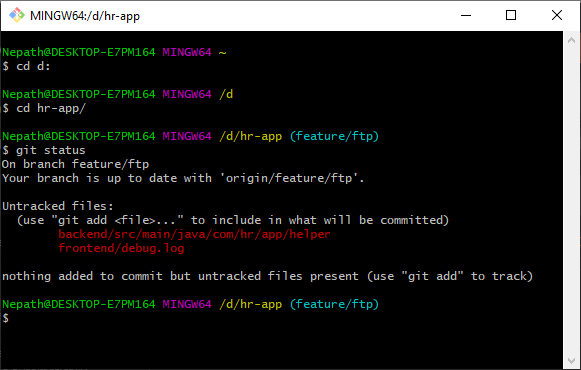
\includegraphics[scale=0.9]{images/gitbash.png}
    \caption{Widok programu \textit{GitBash}. Źródło: Opracowanie własne.}
    \label{fig:gitbash}
\end{figure}
\newpage
Nieodłączną częścią życia programisty, jest stałe pisanie nowego kodu. Jednak, biorąc pod uwagę to, że że nikt nie jest doskonały, może się zdarzyć, że ten pominie jakiś ważny aspekt, który miał zostać zaimplementowany. Problemy pojawiają się częściej, gdy programistą jest osoba na stanowisku młodszego dewelopera (ang. \textit{Junior  Developer}). Osoby niedoświadczone mogą produkować znacznie więcej błędów, które to muszą zostać sprawdzone przez bardziej doświadczonych programistów.\linebreak Te wszystkie problemy sprawiają, że nie można od razu wprowadzić nowych zmian do wersji użytkowej. Rozwiązaniem są gałęzie (ang. \textit{branch}). Za ich pomocą można skopiować główną wersję aplikacji i, nie naruszając głównej gałęzi, ulepszać kod. Następnie, gdy już dane zadanie zostało zakończone, należy wykonać tzw. \textit{pull request}. Funkcja ta pozwala na wdrożenie zaaplikowanych zmian do głównej gałęzi projektu.

W projekcie został użyty \textit{GitHub}, czyli hosting, wykorzystujący system kontroli wersji \textit{Git}. Natomiast, jako program wspomagający wszelkiego rodzaju czynności, został użyty \textit{GitBash}, jak i wbudowane opcje pomocnicze w środowiskach programistycznych, opisanych w dalszej części pracy.

\begin{figure}[h!]
  \centering
  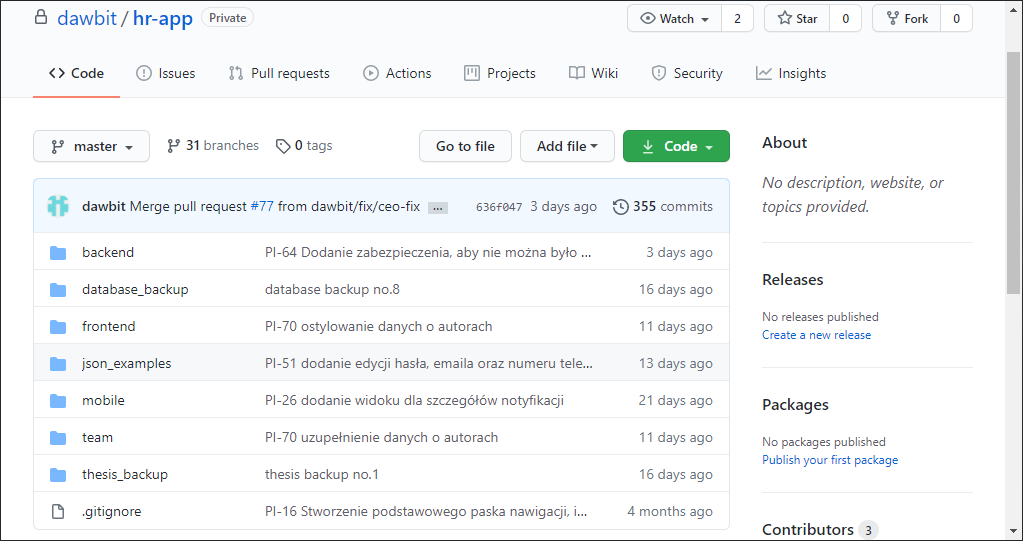
\includegraphics[scale=0.55]{images/github.png}
    \caption{Widok platformy \textit{GitHub}. Źródło: Opracowanie własne.}
    \label{fig:github}
\end{figure}

\subsection{Oprogramowanie do zarządzania projektem}
Podczas wykonywania danego projektu, niezbędną rzeczą jest przypisywanie poszczególnym członkom zespołu odpowiednich zadań. Wprowadza to jasny podział obowiązków w zespole.

\begin{figure}[h!]
  \centering
  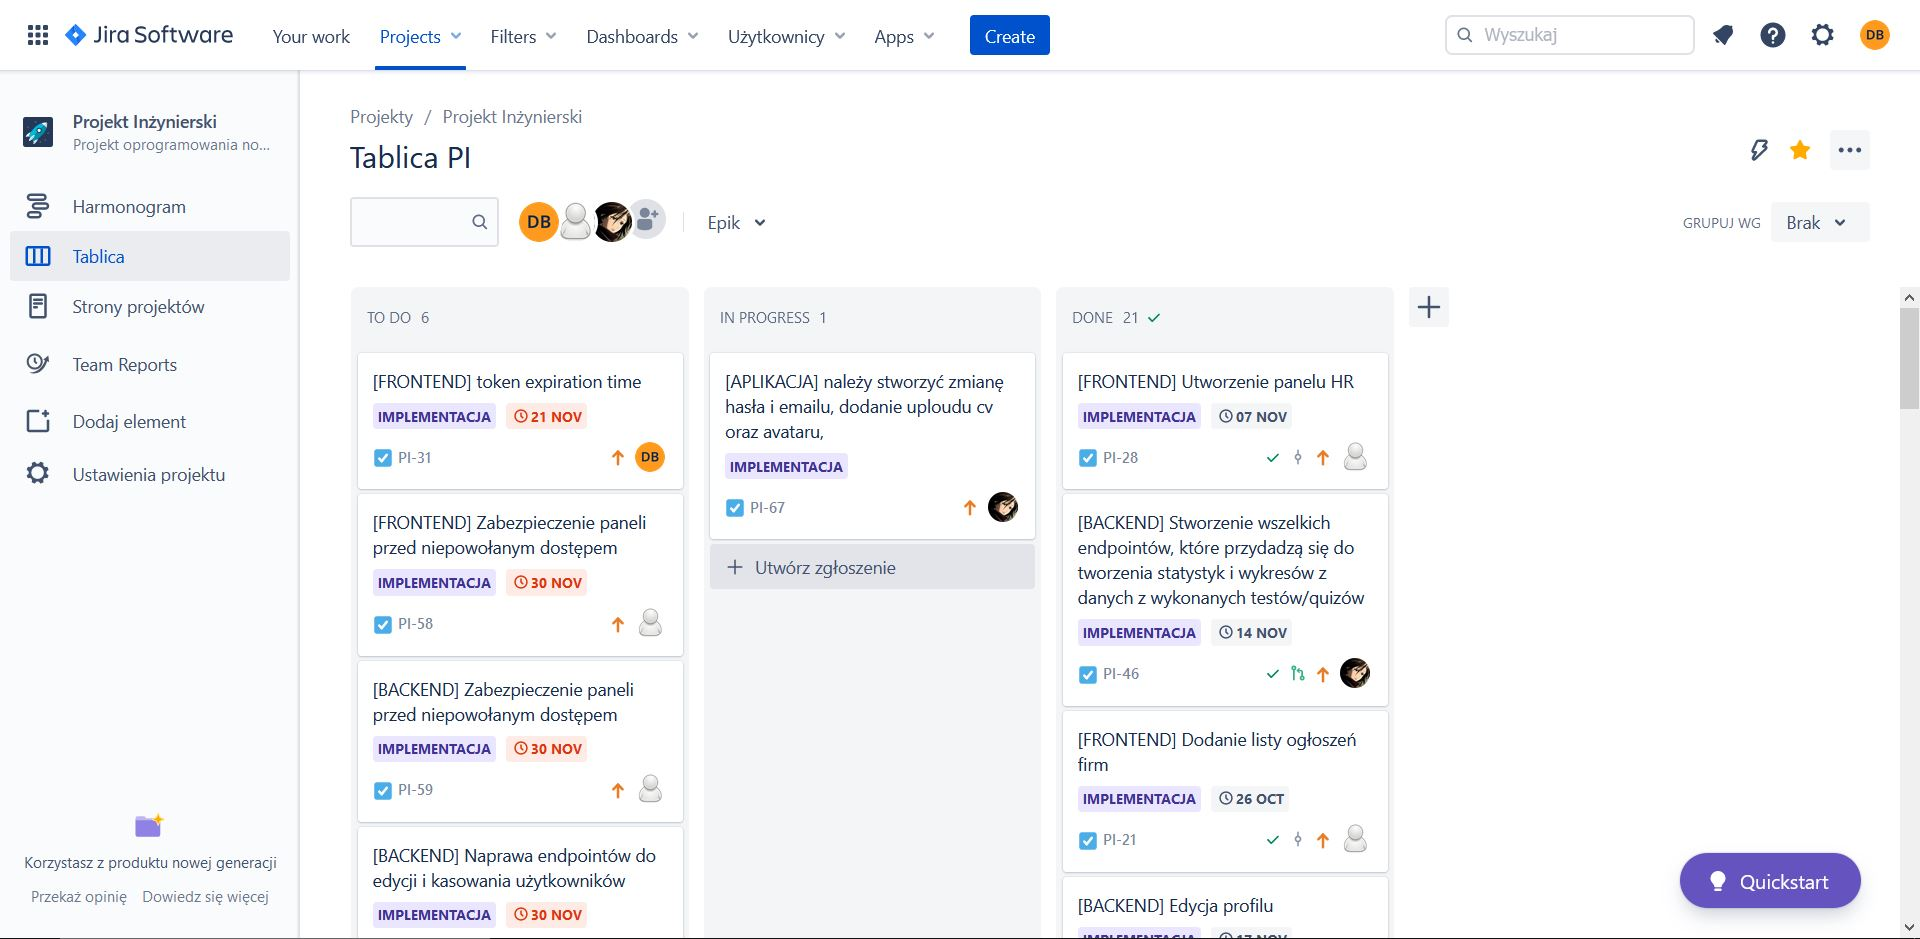
\includegraphics[scale=0.35]{images/jira1.JPG}
    \caption{Główny widok \textit{Jira}. Źródło: Opracowanie własne.}
    \label{fig:jira_main}
\end{figure}

Dzięki systemowi \textit{Jira}, każdy z członków zespołu wie, jakie zadania zostały mu przydzielone oraz ile czasu ma na ich wykonanie. System ten pozwala na kontrolę przepływu pracy w projekcie, członkowie mają wgląd do informacji o tym, jakie zadania są aktualnie wykonywane, jakie zostały zamknięte oraz jakie czekają\linebreak w kolejce.

\begin{figure}[h!]
  \centering
  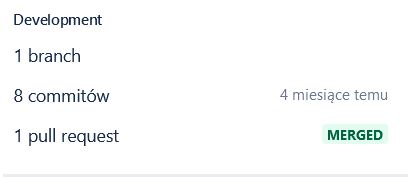
\includegraphics[scale=1]{images/jira4.JPG}
    \caption{\textit{Jira} -- Szczegóły zadania pobranego z wtyczki \textit{GitHub}. Źródło: Opracowanie własne.}
    \label{fig:jira_task_github}
\end{figure}

\newpage

\begin{figure}[h!]
  \centering
  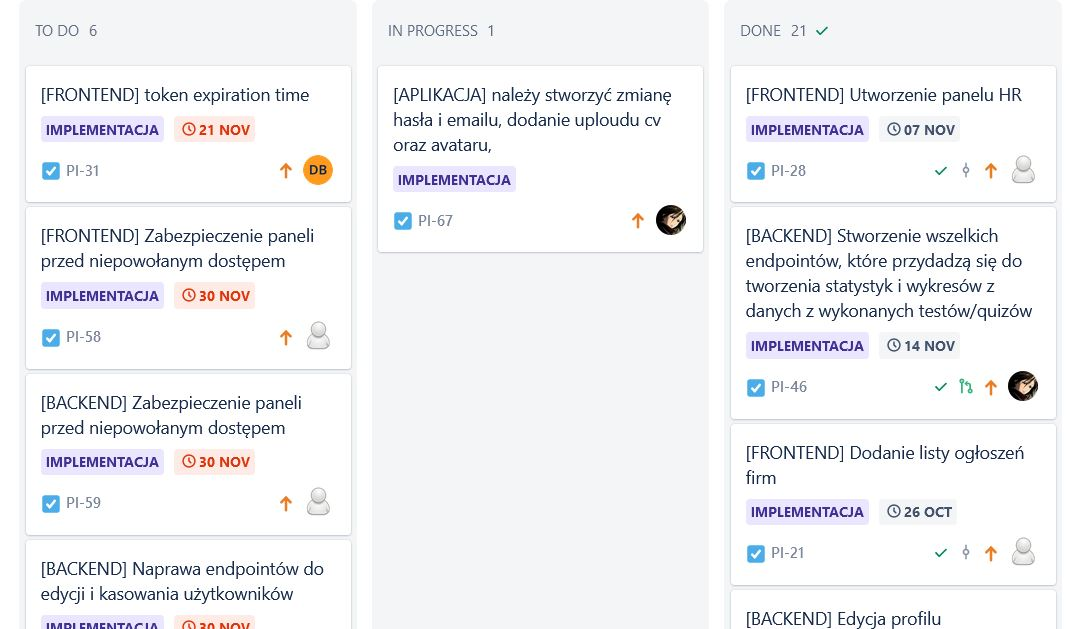
\includegraphics[scale=0.65]{images/jira2.JPG}
    \caption{\textit{Jira} -- Tablica \textit{Agile}. Źródło: Opracowanie własne.}
    \label{fig:jira_agile}
\end{figure}

Jak widać \textit{Jira} to zaawansowane narzędzie, dzięki któremu zyskujemy pełną kontrolę nad realizacją zadań projektowych.

\begin{figure}[h!]
  \centering
  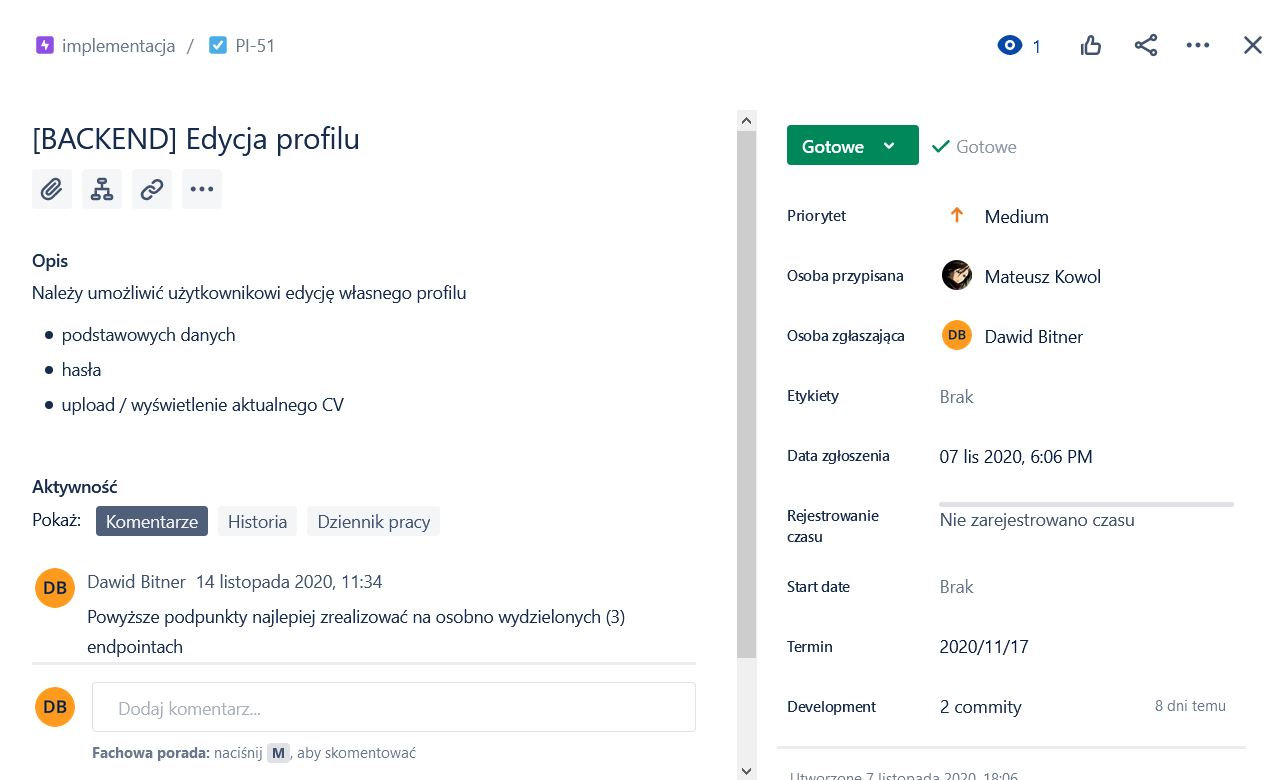
\includegraphics[scale=0.55]{images/jira3.JPG}
    \caption{\textit{Jira} -- Wygląd przykładowego zadania. Źródło: Opracowanie własne.}
    \label{fig:jira_task}
\end{figure}

\newpage

\begin{figure}[h!]
  \centering
  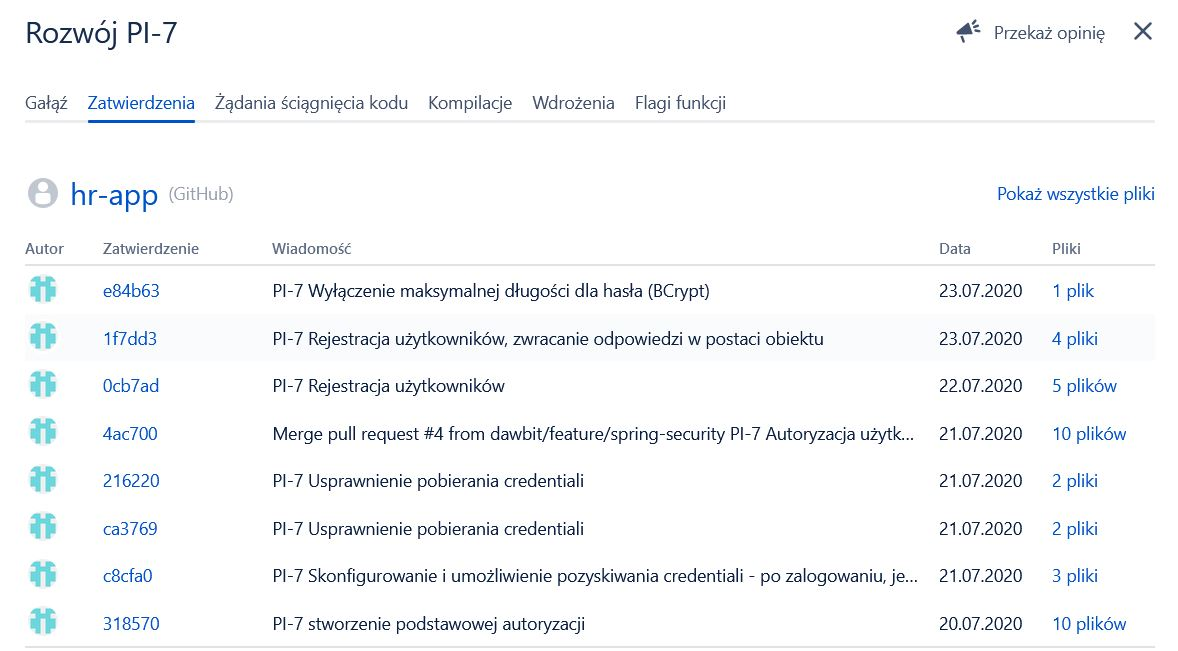
\includegraphics[scale=0.60]{images/jira5.JPG}
    \caption{\textit{Jira} -- Szczegóły przykładowego zadania. Źródło: Opracowanie własne.}
    \label{fig:jira_task_details}
\end{figure}

Dzięki zakładce zatwierdzenia można w przyjazny dla użytkownika sposób,\linebreak w formie listy, podejrzeć zatwierdzone postępy w realizacji danego zadania.

\begin{figure}[h!]
  \centering
  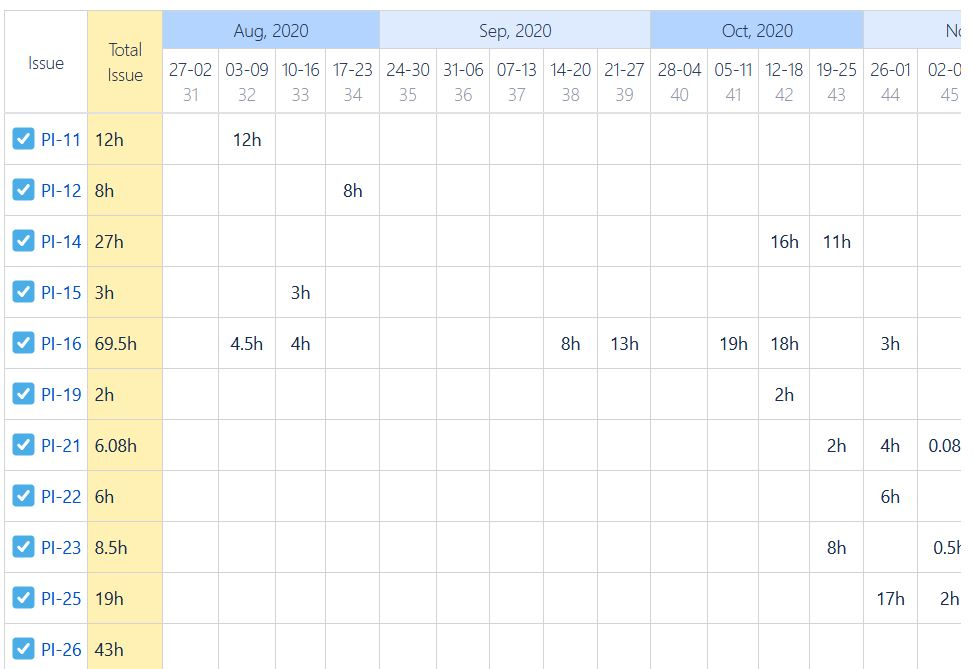
\includegraphics[scale=0.6]{images/jira6.JPG}
    \caption{\textit{Jira} -- Wygląd raportu z użyciem wtyczki \textit{Team Raports}, odnośnie przepracowanego czasu nad zadaniami. Źródło: Opracowanie własne.}
    \label{fig:jira_raport}
\end{figure}

\newpage

\textit{Jira} to łatwy sposób na kontrolę czasu poświęconego na zadania. Z tabeli na rysunku \ref{fig:jira_raport} można na przykład wywnioskować, że zadanie PI-16 było najbardziej skomplikowanym i wymagało dużo uwagi od zespołu projektowego.

\begin{figure}[h!]
  \centering
  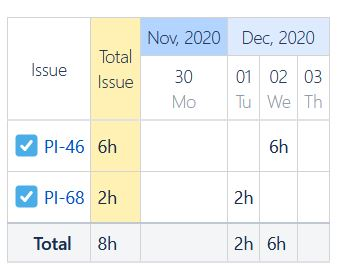
\includegraphics[scale=1]{images/jira7.JPG}
    \caption{\textit{Jira} -- Wygląd raportu w skróconej wersji. Źródło: Opracowanie własne.}
    \label{fig:jira_raport_short}
\end{figure}


\begin{figure}[h!]
  \centering
  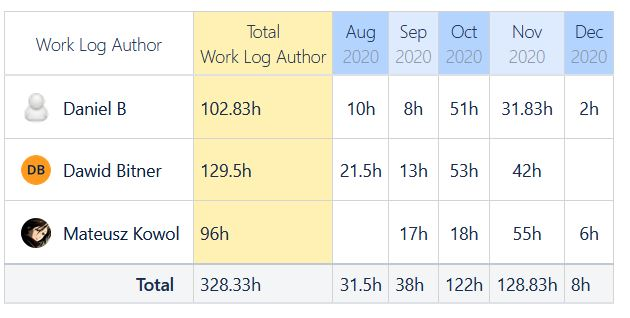
\includegraphics[scale=0.9]{images/jira8.JPG}
    \caption{\textit{Jira} -- raport przepracowanych godzin. Źródło: Opracowanie własne.}
    \label{fig:jira_raport_user}
\end{figure}

\newpage
\subsection{Środowiska programistyczne}
\subsubsection{InteliJ}
\textit{InteliJ} jest środowiskiem programistycznym, stworzonym przez producenta o nazwie \textit{JetBrains} w 2001 roku. Jest doskonałym narzędziem, wspomagającym pisanie w języku \textit{Java}, najchętniej wybieranym przez programistów, którzy są zorientowani właśnie na tą gałąź programowania. Licencje dzielą się na dwie wersje. Wersja pod nazwą \textit{Communnity} jest bezpłatna i różni się od płatnej wersji \textit{Ultimate} tym, że nie oferuje większego wsparcia dla takich struktur, jak \textit{Spring}, \textit{JavaEE} czy \textit{Hibernate}\footnote{Informacje licencyjne firmy Jet Brains, \newline 
\url{https://www.jetbrains.com/idea/buy/\#ommercial?billing=yearly} (dostęp 11.12.2020)}.

\begin{figure}[h!]
  \centering
  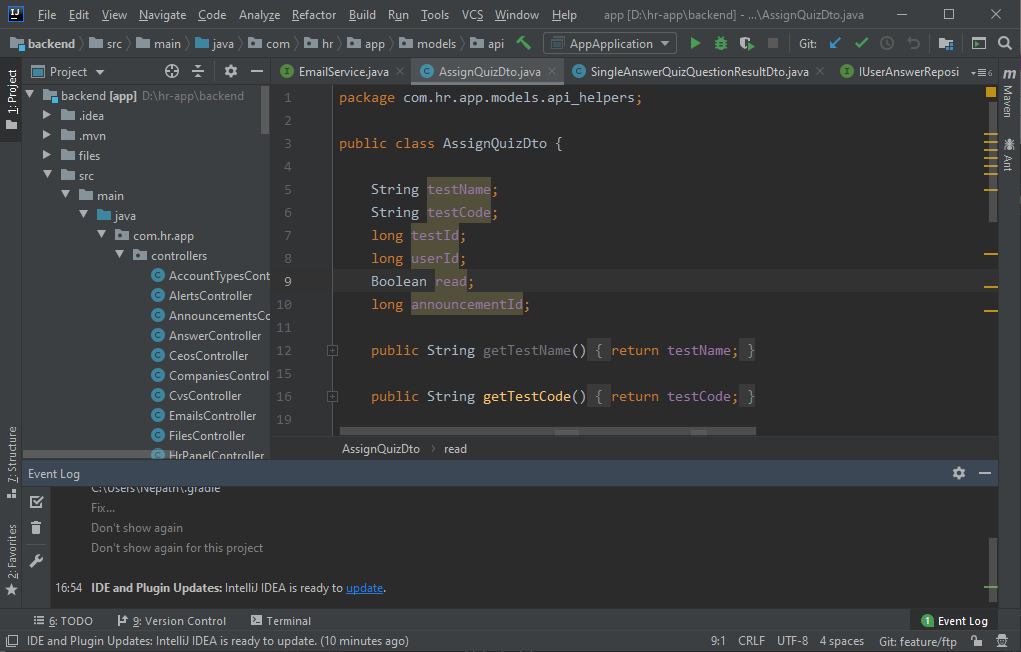
\includegraphics[scale=0.55]{images/intelij.png}
    \caption{Środowisko programistyczne \textit{InteliJ}. Źródło: Opracowanie własne.}
    \label{fig:androidstudio}
\end{figure}

\subsubsection{Visual Studio Code}
Kolejnym narzędziem niezbędnym do stworzenia całego oprogramowania jest platforma, na której w nieskomplikowany sposób można stworzyć widok i logikę dla stron internetowych. Mając na uwadze doświadczenia członków zespołu z poszczególnymi środowiskami, został wybrany \textit{Visual Studio Code}. Środowisko programistyczne stworzyła rozpoznawalna firma \textit{Microsoft} i jest w pełni darmowe\footnote{Warunki licencyjne oprogramowania Microsoft -- Visual Studio Code, \newline 
\url{https://code.visualstudio.com/license} (dostęp 11.12.2020)}.

\begin{figure}[h!]
  \centering
  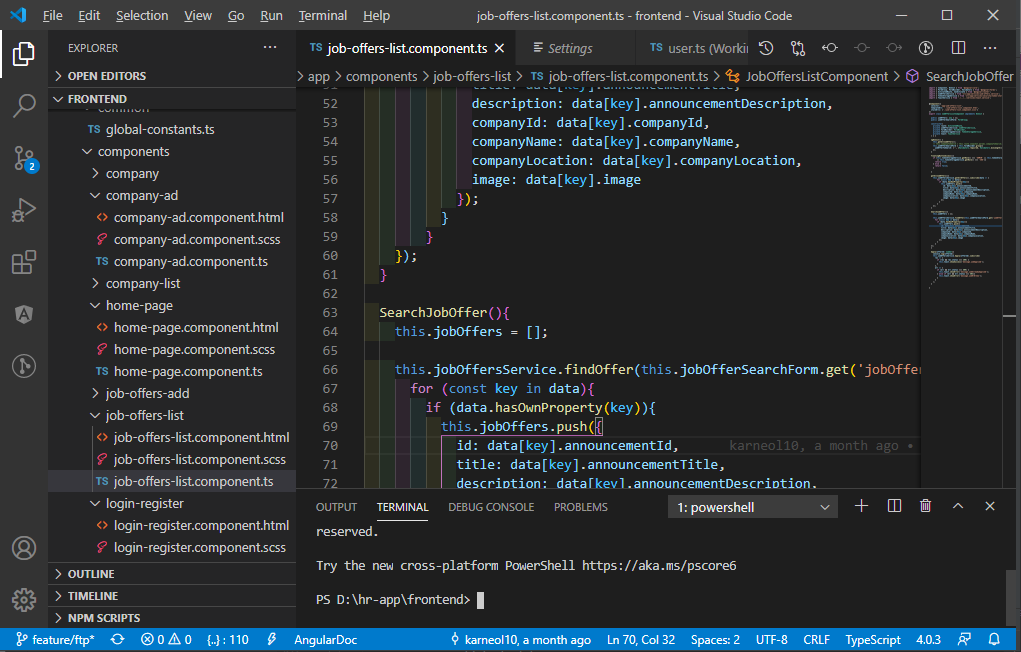
\includegraphics[scale=0.55]{images/visualcode.png}
    \caption{Środowisko programistyczne \textit{Visual Studio Code}. Źródło: Opracowanie własne.}
    \label{fig:visualcode}
\end{figure}

\subsubsection{Android Studio}
Na rynku można znaleźć trzy główne środowiska, wspierające pisanie w platformie programistycznej \textit{Flutter}. Wspomniane już wcześniej \textit{Visual Studio Code}, jest doskonałym środowiskiem dla osób, które mają problemy ze zbyt dużym użyciem pamięci \textit{RAM} w systemie operacyjnym \textit{Windows}. Drugą propozycją jest \textit{Xcode} zaprojektowany przez przedsiębiorstwo \textit{Apple Inc}., jednak ta opcja jest jedynie dostępna dla osób posiadających sprzęt tejże firmy\footnote{Xcode12.2 – umowa licencyjna, \newline
\url{https://apps.apple.com/pl/app/xcode/id497799835?l=pl} (dostęp 11.12.2020)}. Ostatnim środowiskiem, które ostatecznie zostało użyte w projekcie, jest \textit{Android Studio}, korporacji \textit{JetBrains}, oferujące głównie wsparcie dla natywnego pisania w języku \textit{Kotlin}, bądź \textit{Java}, jednak nie ma większych problemów ze wspieraniem języka \textit{Dart}, po zaimplementowaniu odpowiednich wtyczek.

\begin{figure}[h!]
  \centering
  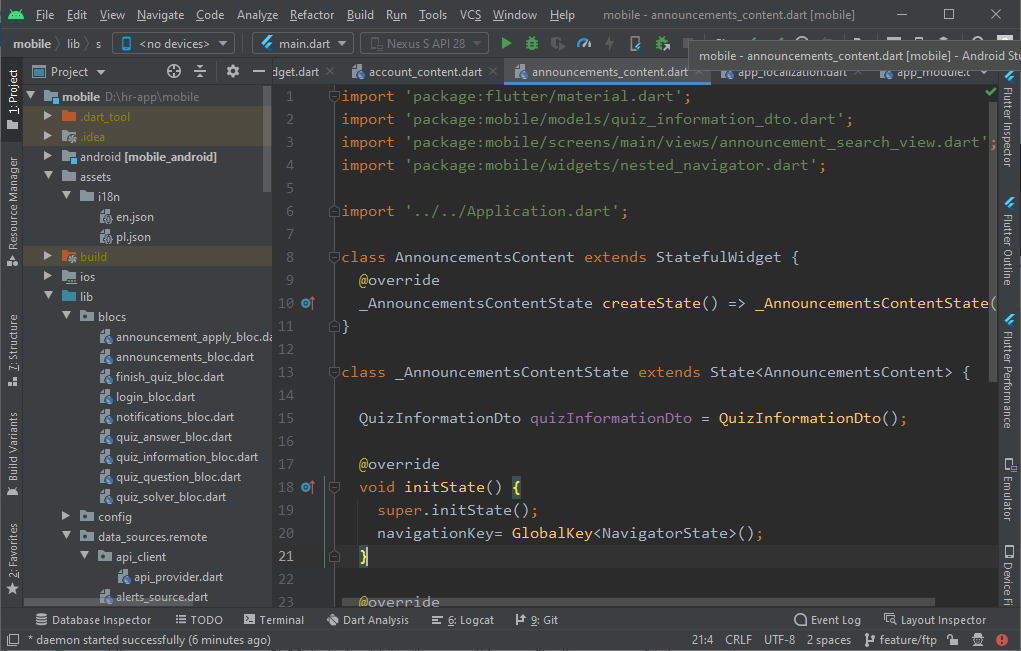
\includegraphics[scale=0.55]{images/androidstudio.png}
    \caption{Środowisko programistyczne \textit{Android Studio}. Źródło: Opracowanie własne.}
    \label{fig:android_studio}
\end{figure}

\subsubsection{PG Admin}
Koniecznym oprogramowaniem w projekcie, w którym została zaimplementowana baza danych typu \textit{PostgreSQL}, jest kompatybilny z tą technologią program \textit{PG Admin}\footnote{Materiały System Administration Portal, „PostgreSQL -- pgAdmin”, \newline
\url{https://pl.admininfo.info/postgresql-pgadmin} (dostęp 11.12.2020)}. Poprzez odpowiednie zintegrowanie środowiska, jest się w stanie w szybki sposób zarządzać bazą danych, śledzić poprawność zmian dokonanych przy pomocy serwera bądź sztywno dodawać, usuwać i edytować elementy, co często przyśpiesza pracę programisty. Pierwsza wersja \textit{PG Admina} została wydana w 1998 roku, przez \textit{pgAdmin Development Team}.

\subsubsection{Postman}
Drugorzędnym środowiskiem, które nie jest konieczne, jednak niezwykle usprawnia testowanie ostatnio wprowadzonych zmian w punktach końcowych, (ang. \textit{end-point}) jest \textit{Postman}. Narzędzie to gwarantuje nam w prosty sposób dostęp do takich zasobów jak: nagłówki, ciało wysyłanego żądania, czy również wspomaga wysyłanie całych plików na serwer. Nie można zapomnieć o zwrotnych informacjach, które oferuje platforma i są one wyświetlane w czytelny sposób. \textit{Postman} został wydany w 2014 roku przez firmę \textit{Postman inc}.

\begin{figure}[h!]
  \centering
  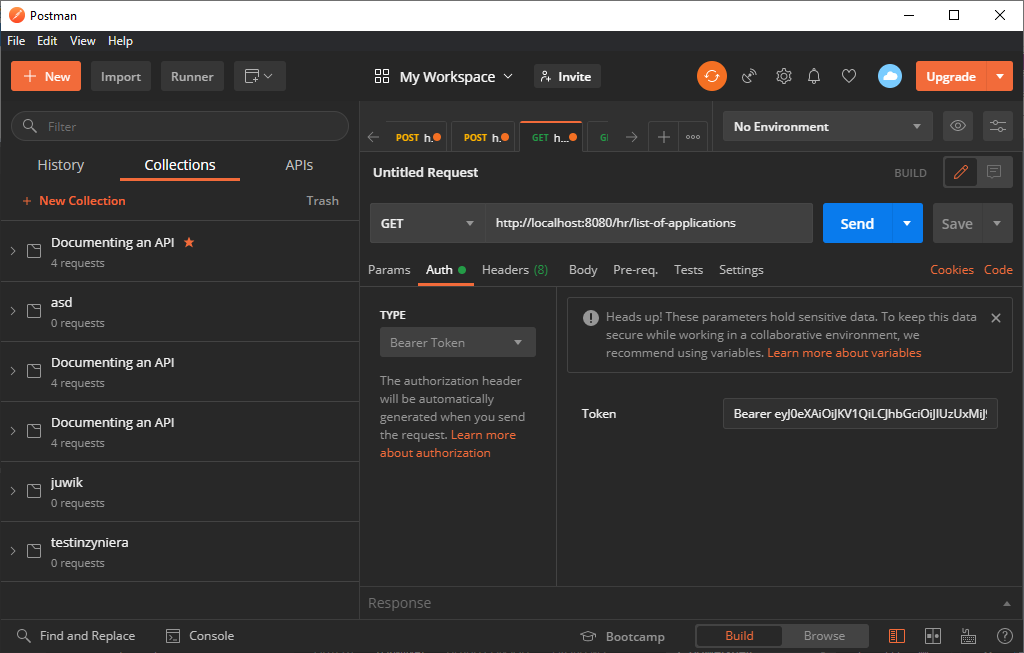
\includegraphics[scale=0.55]{images/postman.png}
    \caption{Program wspomagający \textit{Postman}. Źródło: Opracowanie własne.}
    \label{fig:postman}
\end{figure}

\section{Specyfikacja}
Sekcja przedstawia informacje odnośnie instalacji poszczególnych komponentów, potrzebnych do uruchomienia stworzonego systemu oraz instrukcję obsługi części serwerowej, mobilnej i przeglądarkowej.

\subsection{Instalacja i konfiguracja środowisk}
Przed przystąpieniem do tworzenia aplikacji, należy pobrać odpowiednie środowiska dla poszczególnych części projektu tj. zaplecza, części webowej oraz aplikacji mobilnej, zwracając przy tym uwagę na wybieraną licencję.

\subsubsection{InteliJ IDEA}
Aby pobrać środowisko do pracy z kodem \textit{Java (Spring Boot)}, należy udać się na stronę: \url{https://www.jetbrains.com/idea/download/\#section=windows}, a następnie wybrać bezpłatną wersję społecznościową (ang. \textit{Community}). Później należy przeprowadzić standardową instalację oprogramowania na aktualnym systemie operacyjnym. Po zakończeniu instalacji należy uruchomić środowisko, a następnie,\linebreak w ustawieniach kompilatora, wskazać ścieżkę do folderu głównego \textit{Javy}.

\subsubsection{Visual Studio Code}
\textit{Visual Studio Code} można pobrać z oficjalnej strony producenta \textit{Microsoft}:
\url{https://code.visualstudio.com/}. Jako że edytor nie posiada wbudowanych wtyczek do pracy ze środowiskiem \textit{Angular}, należy wyszukać odpowiednie wtyczki\linebreak w zakładce rozszerzeń. Do pracy z \textit{Angularem} przydatne mogą być takie wtyczki jak np. zestaw \textit{Angular Extension Pack}, czy rozszerzenia wspomagające debugowanie\linebreak w przeglądarkach, np. \textit{Debugger for Chrome}.

\subsubsection{Android Studio}
W celu zainstalowania środowiska Android Studio, należy udać się na stronę:
\url{https://developer.android.com/studio}, gdzie znajduje się odnośnik do najnowszej wersji programu. Po standardowej instalacji, opcjonalną rzeczą jest dodanie emulatora, czyli wirtualnego telefonu z systemem Android, symulującego zachowanie prawdziwego telefonu. W tym celu, z listy rozwijanej, w górnej części aplikacji, gdzie znajduje się informacja o braku dostępnych urządzeń, należy wybrać opcję \textit{AVD Manager}. Następnie z dostępnych urządzeń należy wybrać jedno, przejść dalej, zdecydować która wersja \textit{Androida} jest pożądana, ilość pamięci \textit{RAM}, którą chcemy przeznaczyć dla emulatora i go zainstalować.

\subsubsection{Postman}
Narzędzie \textit{Postman} można pobrać ze strony internetowej, znajdującej się pod adresem: \url{https://www.postman.com/downloads/}. Instalację należy przeprowadzić w sposób standardowy.

\subsubsection{GitBash}
Można pobrać oprogramowanie do systemu kontroli wersji. Jest to jednak opcjonalne, ponieważ jest ono wbudowane zarówno w \textit{Visual Studio Code}, jak i \textit{Android Studio}, czy \textit{InteliJ IDEA}. Aby zainstalować program, należy pobrać plik instalacyjny ze strony producenta: \url{https://git-scm.com/downloads}. Po instalacji użytkownik dostaje dostęp do \textit{Git GUI} oraz \textit{Git Bash}, które służą do wykonywania poleceń \textit{git}.

\subsubsection{PostgreSQL}
Do zainstalowania silnika baz danych \textit{PosgreSQL} oraz narzędzia do zarządzania bazą wykonanych zapytań -- \textit{pgAdmin4}, należy odwiedzić stronę internetową:
\url{https://www.enterprisedb.com/downloads/postgres-postgresql-downloads}.
Następnie należy wybrać plik instalacyjny najnowszej wersji, zgodny z systemem operacyjnym, na którym program ma zostać zainstalowany. Podczas instalacji użytkownik powinien wybrać komponent opcjonalny \textit{pgAdmin4}.

Po udanym pobraniu i zainstalowaniu należy przejść do folderu w którym serwer został umieszczony, a następnie wybieramy folder \textit{bin}, z którego można utworzyć skrót do aplikacji \textit{pgAdmin4.exe} na pulpicie.

\subsubsection{Java}
W celu zainstalowania \textit{Javy} należy pobrać ją ze strony producenta:
\url{https://www.java.com/pl/download/}. Po przejściu przez standardową instalację, podczas której użytkownik powinien zdecydować, w którym miejscu chcemy zainstalować oprogramowanie, należy dodać je do zmiennych środowiskowych. W tym celu należy wybrać w \textit{Menu Start} komponent \textit{Edytuj zmienne środowiskowe}. Gdy pojawi się okienko, kolejnym krokiem jest przejście do zakładki \textit{Zaawansowane}, po czym wybranie \textit{Zmienne środowiskowe...}. Należy dodać nową zmienną o nazwie \textit{JAVA\_HOME}, a jako wartość wpisać ścieżkę do folderu w którym \textit{Java} została zainstalowana.

\subsubsection{Node.js}
Aby korzystać z platformy programistycznej \textit{Angular}, niezbędne jest posiadanie środowiska \textit{node.js}. W tym celu należy odwiedzić oficjalną stronę oprogramowania: \url{https://nodejs.org/en/}. Po pobraniu najnowszej wersji (zalecana jest wersja o długim wsparciu (ang. \textit{Long Time Support (LTS)}) należy wywołać instalator\linebreak i przejść standardową instalację. W celu weryfikacji prawidłowego przebiegu instalacji należy wpisać w wierszu poleceń następujące polecenia: \textbf{node -v} oraz \textbf{npm -v}. Jeżeli wszystko zostało poprawnie wykonane, zostanie zwrócony numer wersji.

\subsubsection{Angular}
W celu instalacji platformy programistycznej \textit{Angular} należy uruchomić konsolę systemową i wykonać następujące polecenie: \textbf{npm install -g @angular/cli}.

\subsubsection{Flutter}
Aby móc korzystać z platformy programistycznej \textit{Flutter}, podstawowym krokiem jest pobranie pliku \textit{.zip} ze strony: \url{https://flutter.dev/docs/get-started/install}, a następnie wypakować go do rekomendowanej przez \textit{Google} ścieżki \linebreak\textit{C:\textbackslash src\textbackslash flutter}.

Kolejnym krokiem jest przejście do zmiennych środowiskowych. \textit{Dokładna instrukcja, jak tego dokonać znajduje się w punkcie 7.1.7}. W tym miejscu, do zmiennej o nazwie \textit{Path} należy dodać nową ścieżkę, która odpowiada miejscu zapisanego oprogramowania. Jeżeli wszystko przebiegło pomyślnie, po wpisaniu komendy \textbf{flutter --version} w wierszu poleceń, ukaże się informacja o wersji \textit{Fluttera}. 

\subsection{Instrukcja obsługi}
W tej części podrozdziału zawarte są podstawowe informacje, które dotyczą instrukcji obsługi poszczególnych części projektowych.

\subsubsection{Część serwerowa}
Aby uruchomić serwer, należy posiadać na docelowym sprzęcie zainstalowany serwer bazodanowy \textit{PostgreSQL}, a następnie uruchomić aplikację \textit{Hr-App.jar}, która jest dostępna u twórców projektu. Gdy serwer się uruchomi, można bezproblemowo się z nim połączyć, o ile użytkownik używa tej samej sieci, w której się znajduje lub zmodyfikować ją, by była ogólnodostępna. Istnieje również możliwość produkcyjnego wystawienia serwera do sieci, przy pomocy np.: kontenera aplikacyjnego \textit{Apache Tomcat}. W takim przypadku, wystarczy, że pliki aplikacji znajdą się w odpowiednim podfolderze \textit{Tomcata} oraz że serwer jest uruchomiony.


\subsubsection{Część internetowa}
Aby uruchomić serwer, odpowiedzialny za dostęp użytkownika do strony internetowej, należy  otworzyć folder \textit{frontend} w programie \textit{Microsoft Visual Studio Code} i w konsoli wykonać komendę \textbf{ng serve $--$open}, która spowoduje kompilację kodu i włączenie domyślnej przeglądarki internetowej, z otwartą zakładką aplikacji.
Istnieje również możliwość wdrożenia części internetowej aplikacji na serwer. Aby tego dokonać, należy analogicznie, lecz zamiast komendy \textbf{ng serve $--$open}, użyć \textbf{ng build}, która spowoduje kompilację kodu i wygeneruje pliki, niezbędne do jej uruchomienia na serwerze własnego wyboru. Po udostępnieniu strony za pomocą własnego hostingu, można się z nią połączyć, wpisując w przeglądarce internetowej ustalony przez hosting adres.

\subsubsection{Część mobilna}

Aby korzystać z oprogramowania na swoim telefonie, należy na nim uruchomić otrzymany plik \textit{Hr-App.apk} i zainstalować zawartość. Gdy wszystko przebiegnie pomyślnie, wyświetli się okno aplikacji. Po pojawieniu się okna logowania, należy się zarejestrować bądź zalogować. Następnie, po udanej autoryzacji, użytkownik zostanie przeniesiony do widoku głównego kontentu aplikacji.

\section{Implementacja}
Rozdział przedstawia najważniejsze informacje, które dotyczą implementacji projektu, z podziałem na część serwerową i kliencką, w postaci aplikacji mobilnej\linebreak i przeglądarkowej.

\subsection{Serwer}
Część serwerowa odpowiada za obsługę bazy danych oraz działań użytkownika\linebreak z nią związanych, takich jak np.: obsługa rozwiązywania quizów, zwracanie tabel, zabezpieczenia i inne. Najważniejsze cechy zaplecza, jak i pozostałych części aplikacji, zostały omówione w tym podrozdziale.

\subsubsection{Specyfikacja bazy danych}
Pomysł oraz budowa bazy danych zostały omówione w rozdziale \textbf{3.1}. Samo tworzenie bazy danych obyło się bez tworzenia podzapytań \textit{SQL}. Zapytania pisane ręcznie są wykorzystywane tylko w kilku specyficznych przypadkach, w których zapytanie \textit{JPASQL}, z wykorzystaniem zapytań wbudowanych, było zbyt skomplikowane lub zbyt długie, co negatywnie wpływało na czytelność kodu. Zapytania \textit{Spring Data JPA} umożliwiają tworzenie zapytań, które składają się z nazwy akcji, jak np.: \textit{find…By}, \textit{count…By} lub \textit{delete…By} i nazwy pól encji. Przykładowo:
\begin{lstlisting}[language=Java,caption=Kod źródłowy wysyłający zapytanie do bazy o ilość nieodczytanych powiadomień dla działu HR danej firmy. Źródło: Opracowanie własne. ,captionpos=b]
    long countByReadAndFKhrAlertAnnouncementFKannouncement
         CompanyId(boolean read, long companyId);
\end{lstlisting}
zwróci liczbę powiadomień użytkownikowi działu HR, na podstawie tego, czy chce on zwrócić liczbę odczytanych czy nieodczytanych oraz na podstawie identyfikatora firmy.
Wszystkie zapytania znajdują się w repozytoriach, które zostały rozszerzone o klasę \textit{JpaRepository}, umożliwiającą wykonywanie tego typu działań.
Natomiast, własne, natywne zapytanie wygląda w następujący sposób:

\newpage

\begin{lstlisting}[caption=Natywne zapytanie do bazy danych w celu pobrania konkretnych informacji. Źródło: Opracowanie własne. ,captionpos=b]
    @Query(value = "SELECT * FROM Announcements announcement 
        JOIN Companies company " +
        "ON company.id = announcement.company_id " +
        "WHERE LOWER(announcement.title) 
        LIKE LOWER(CONCAT('%', ?1,'%')) " +
        "OR LOWER(announcement.description) 
        LIKE LOWER(CONCAT('%', ?1,'%')) " +
        "OR LOWER(company.name) 
        LIKE LOWER(CONCAT('%', ?1,'%')) " +
        "OR LOWER(company.about) 
        LIKE LOWER(CONCAT('%', ?1,'%')) " +
        "OR LOWER(company.location) 
        LIKE LOWER(CONCAT('%', ?1,'%'))", 
        nativeQuery = true
    )
List<AnnouncementsModel> findAnnouncementByAnything(
    String value);
\end{lstlisting}
W tym przypadku zostanie zwrócona lista ogłoszeń, na podstawie wpisanego ciągu znaków, który może zawierać się w: nazwie ogłoszenia, opisie ogłoszenia, nazwie firmy, opisie firmy lub lokalizacji firmy. Rozwiązanie to zostało wykorzystane\linebreak w szybkiej wyszukiwarce ogłoszeń, na podstawie powyższych kryteriów.

\subsubsection{Projekt bazy danych}
W pierwszej kolejności, baza danych została zaprojektowana na kartce, następnie zespół przeszedł do implementacji struktury bazy danych poprzez tworzenie klas\linebreak w projekcie oraz zależności pomiędzy tymi klasami. W dalszej kolejności, zostały wychwycone błędy z początkowej fazy projektu oraz naniesiono odpowiednie poprawki. Stworzenie struktur danych było pierwszym etapem początkowej fazy projektu.

Oprócz błędów związanych z logiką łączeń, zespół napotkał problem z tworzeniem zapytań \textit{JPA} za pomocą metod wbudowanych. Metody te nie radzą sobie\linebreak z tworzeniem zapytań w momencie, kiedy w nazwie kolumny znajduje się myślnik. Myślniki zostały zamienione na znaki podkreślenia.

\paragraph{Diagram związków encji}
\!

Na kolejnych stronach zostały przedstawione diagramy związków encji. Główny – zawierający całą strukturę bazy danych oraz dwa pomniejsze – zawierające wyszczególnione informacje, odnośnie najważniejszych tabel w bazie: kolejno testy\linebreak i użytkownicy.

\begin{figure}[h!]
    \centering
    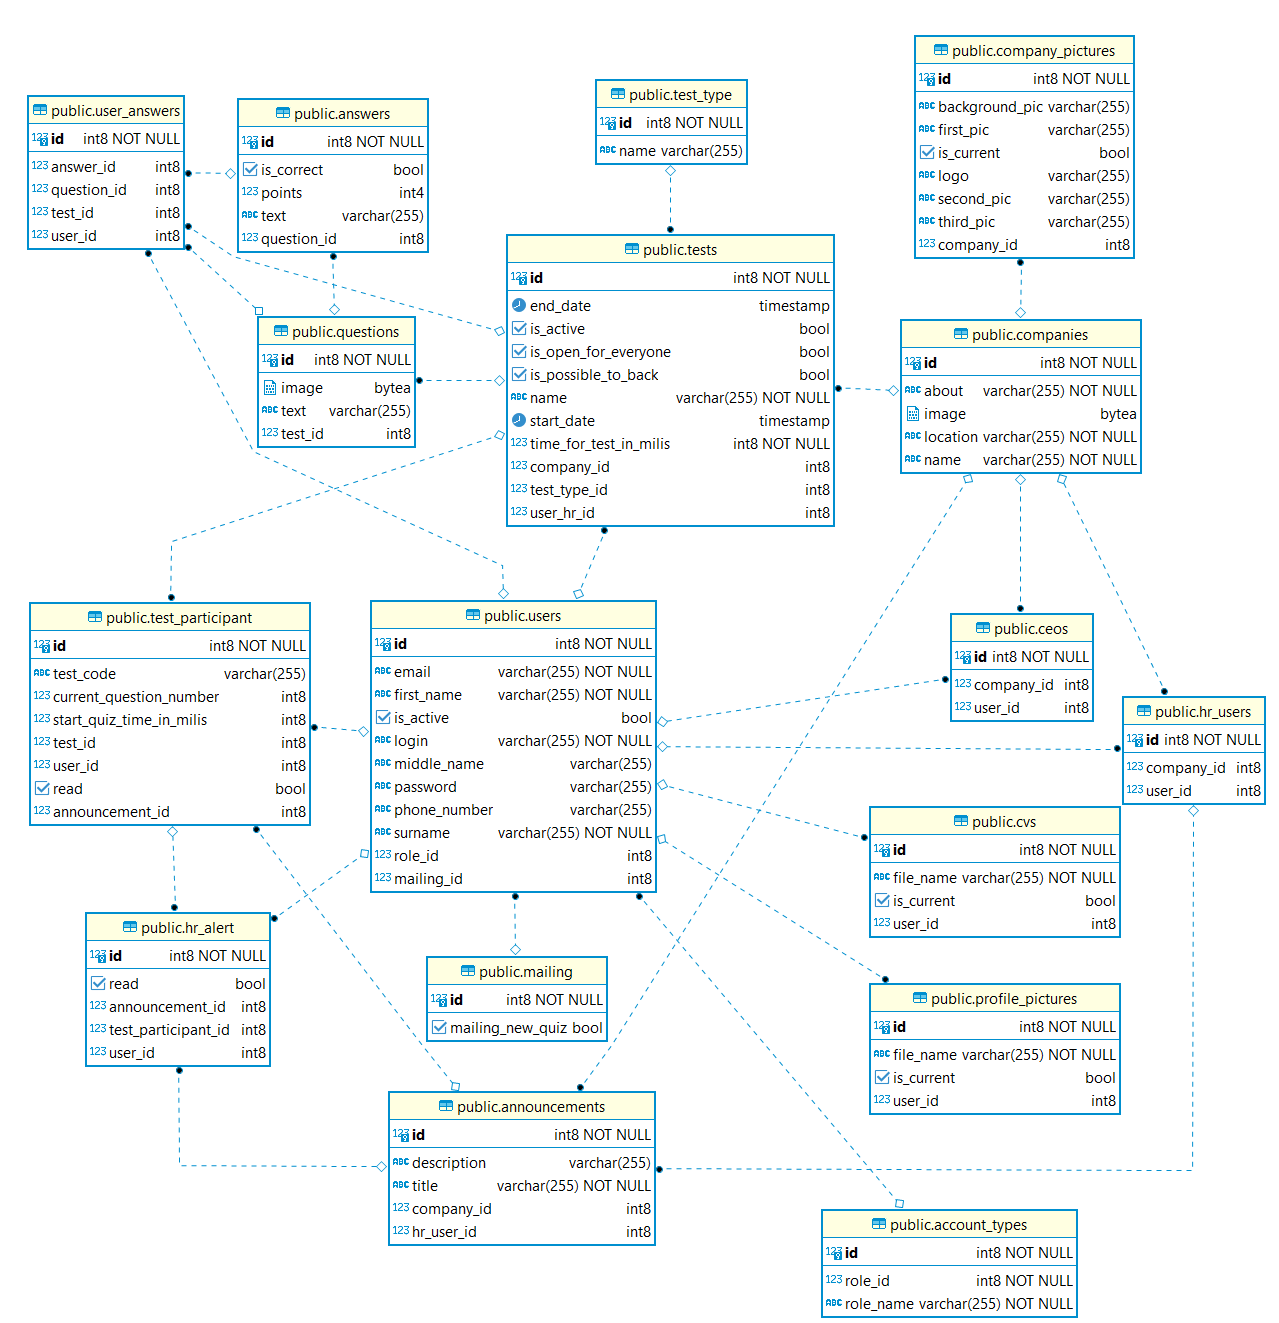
\includegraphics[width=\textwidth]{images/baza.png}
    \caption{Diagram związków encji. Źródło: Opracowanie własne.}
    \label{fig:baza}
\end{figure}

\newpage

\begin{figure}[h!]
    \centering
    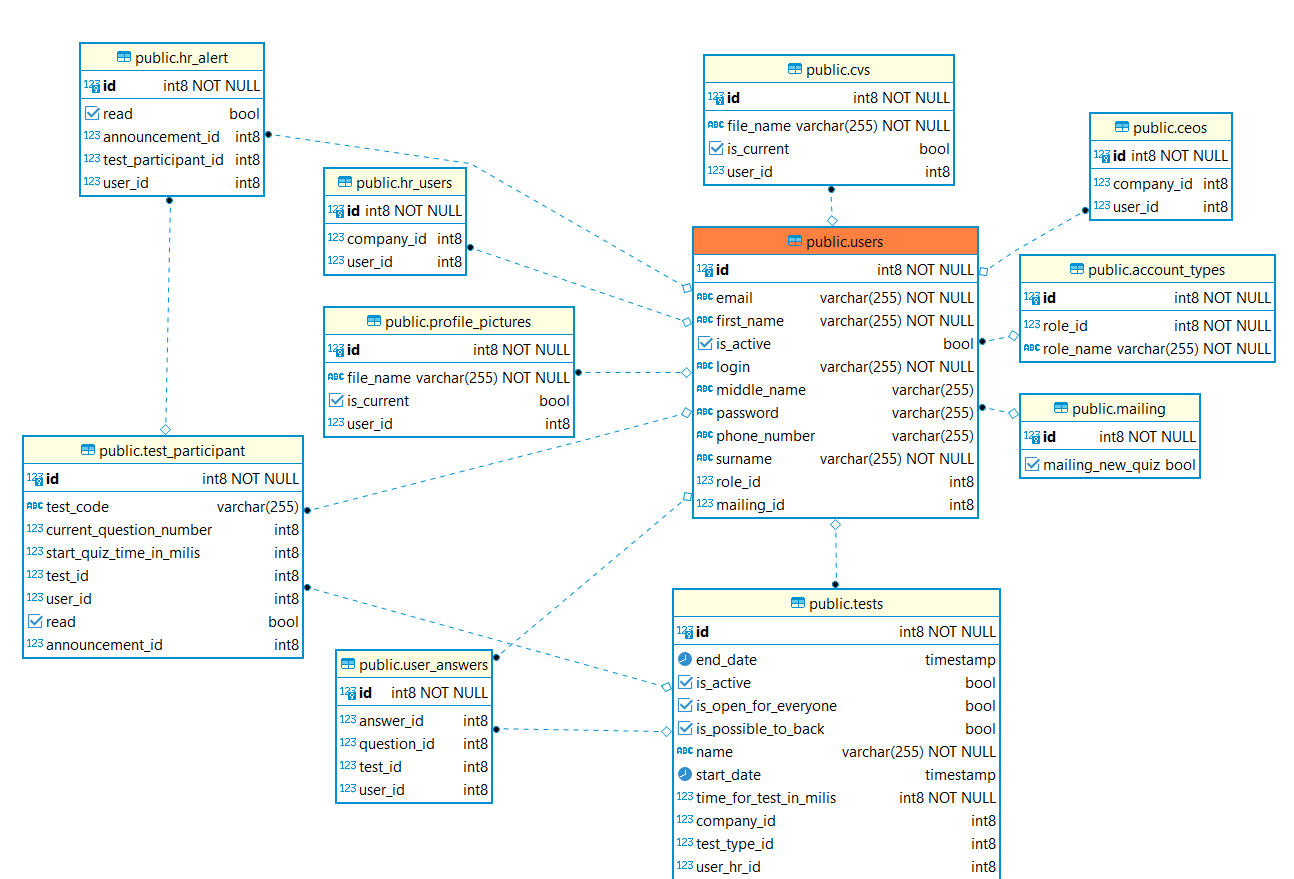
\includegraphics[width=\textwidth]{images/erp_users.png}
    \caption{Diagram związków encji -- tabela użytkowników. Źródło: Opracowanie własne.}
    \label{fig:erp_tests}
\end{figure}

\begin{figure}[h!]
    \centering
    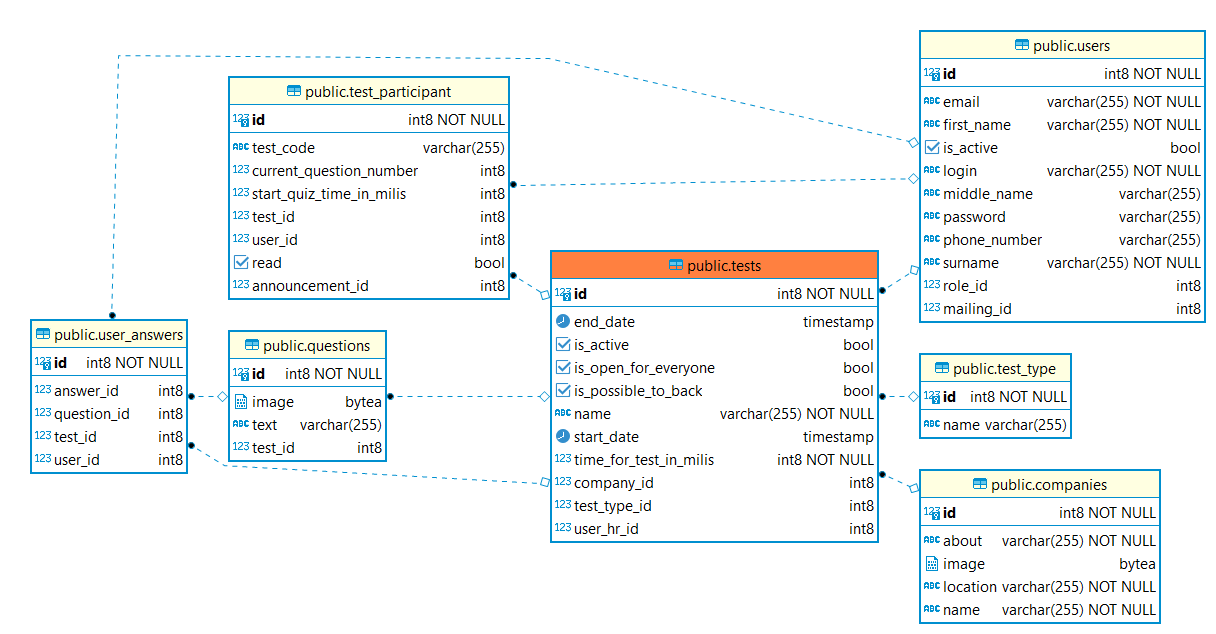
\includegraphics[width=\textwidth]{images/erp_tests.png}
    \caption{Diagram związków encji -- tabela testów. Źródło: Opracowanie własne.}
    \label{fig:erp_users}
\end{figure}

\subsubsection{Spring Security i bcrypt}
W projekcie zostały wykorzystane algorytmy szyfrujące, służące m.in. do zabezpieczenia haseł użytkowników. Został również zaimplementowany system autoryzacji użytkowników za pomocą \textit{JSON Web Tokenu}.

\begin{description}
    \item[Spring Security i JSON Web Token] – \textit{Spring Security} dostarcza zbiór narzędzi, który pozwala na zabezpieczenie tworzonej aplikacji z wykorzystaniem gotowych mechanizmów. Dlatego, w prosty sposób i przy niskim nakładzie pracy programisty, można wykorzystać rozwiązania zaimplementowane w \textit{Spring Security} do autoryzacji, w tym autoryzacji dwuetapowej, poprzez hashowanie danych, \textit{OAuth2}, \textit{JWT}, czy \textit{OpenID}.\newline
    W projekcie, w celu autoryzacji użytkowników, został wykorzystany \textit{JSON Web Token}.
    \begin{lstlisting}[language=Java,caption=Przykład danych w formacie JSON wysyłane przy logowaniu. Źródło: Opracowanie własne.,captionpos=b]
    {
        "login": "x",
        "password": "y"
    }
    \end{lstlisting}
    Gdzie \textit{x} i \textit{y} to kolejno nazwa użytkownika i hasło, na punkt końcowy: \textit{/login}, użytkownik w odpowiedzi dostaje nagłówek \textit{Authorization} z zawartością w postaci \textit{Bearer $<$token$>$}, gdzie \textit{$<$token$>$} to token \textit{JWT}. Zawiera on dane m.in.: o czasie jego przydatności, jak i o uprawnieniach użytkownika do wybranych zasobów. Następnie jest on doczepiany do nagłówków pozostałych zapytań \textit{REST}\footnote{A. Rahmatulloh, „Performance comparison of signed algorithms on JSON Web Token”, 2019,  \newline \url{https://iopscience.iop.org/article/10.1088/1757-899X/550/1/012023/pdf},\newline (dostęp 12.12.2020)}. Bez tego, serwer nie jest w stanie stwierdzić, czy użytkownik posiada poświadczenia do wybranych zasobów. Jeżeli token okaże się nieprawidłowy, wygraśnie lub użytkownik spróbuje dostać się do zasobów, do których nie ma uprawnień, i zostanie zwrócony błąd \textit{http 403} – zabroniona wartość (ang. \textit{forbidden}) – oznacza to, że serwer zrozumiał żądanie (czyli jest skonstruowane poprawnie), ale odmówił użytkownikowi dostępu\linebreak do zasobów.
    Sama zawartość tokenu składa się z trzech części: nagłówku, właściwej zawartości (ang. \textit{payload}) i podpisu. Każda z części jest łączona kropkami, a następnie szyfrowana. 
    
    \begin{figure}[h!]
        \centering
        
\includegraphics[width=\textwidth]{images/jwt.png}
        \caption{Graficzne przedstawienie budowy \textit{JSON Web Tokenu}. Źródło: Opracowanie własne.}
        \label{fig:jwt}
    \end{figure}
    
    Sekcja nagłówkowa składa się z dwóch części: zastosowanego algorytmu i typu tokenu. Zawartość jest kodowana za pomocą \textit{Base64}. Druga część to właściwa zawartość, zawierająca roszczenie o dostęp, które zawiera dane użytkownika,\linebreak w tym nazwę użytkownika i hasło. Ta część również szyfrowana jest w \textit{Base64}. Trzecia część to sygnatura, zawierająca zakodowany nagłówek, zakodowany ładunek, sekretny klucz (który definiowany jest po stronie serwera), a także algorytm, który został zdefiniowany w nagłówku. W tym projekcie zastosowano algorytm kryptograficzny \textit{HMAC}, używający \textit{RSA256}\footnote{A. Michalczyk -- Sekurak, „Kompendium bezpieczeństwa haseł – atak i obrona (część 1.)”, \newline \url{https://sekurak.pl/kompendium-bezpieczenstwa-hasel-atak-i-obrona/},\newline (dostęp 12.12.2020)}.
    
    \begin{equ}[h!]
        \[\textbf{Token} = f(Kodowanie Base64)\displaystyle\sum_{n=\alpha,\beta}^{\infty} (naglowek.wlasciwa\_zawartosc.sygnatura) \]
        \caption{Matematyczne przedstawienie tworzenia tokenu.}
    \end{equ}
    
    \begin{lstlisting}[language=Java,caption=Budowa nagłówka JWT. Źródło: Opracowanie własne.,captionpos=b]
    { "alg": "HS256", "typ": "JWT" }
\end{lstlisting}
    Gdzie \textit{alg} to wykorzystany algorytm do szyfrowania. \newline
    
        \begin{lstlisting}[language=Java,caption=Właściwa zawartość tokenu. Źródło: Opracowanie własne. ,captionpos=b]
    {
        "login": "user1",
        "iat": 1422779222,
        "password": 12345
    }
\end{lstlisting}
    W części właściwej administrator systemu definiuje, jakie dane są przekazywane. Następnie dwie powyższe zawartości są szyfrowane w sygnaturze.
    
    \item[bcrypt] – w projekcie został wykorzystany, w celu bezpiecznego przechowywania haseł użytkowników w bazie danych, w postaci zaszyfrowanej.
    
    \begin{lstlisting}[caption=Sposób w jaki jest zapisywany ciąg bcrypt. Źródło: Opracowanie własne.,captionpos=b]
[identyfikator algorytmu][koszt][22 znaki soli]
[31 znaków hashu]
    \end{lstlisting}
    Na przykład:
    \begin{lstlisting}[caption=Przykładowy ciąg bcrypt. Źródło: Opracowanie własne.,captionpos=b]
$2a$10$N9qo8uLOickgx2ZMRZoMyeIjZAgcfl7p92ldGxadL17lhWy 
\__/\/\____________________/\_______________________/
alg koszt       sól                  hasz
    \end{lstlisting}
Gdzie: \newline
    – \textbf{alg} – wyznacza rodzaj algorytmu, gdzie \textit{\$2a\$} oznacza zmodyfikowany algorytm \textit{Blowfish}. \newline
    – \textbf{koszt} – to współczynnik kosztu. Czyli informacja o tym, ile razy należy uruchomić podany \textit{hash}. Im wyższa wartość, tym odczytywanie hasła jest powolniejsze, ale zwiększona zostaje odporność na ataki brutalne. \newline
    – \textbf{sól} – to ciąg zaburzający. Są to losowe dane dodawane do hasła, które mają zwiększać ochronę przed atakami słownikowymi. Zapisana jest w danych 128 bitowych, zakodowana do 22 znaków \textit{Base64}. \newline
    – \textbf{hasz} – powstaje w wyniku użycia funkcji skrótu. Jest to funkcja przyporządkowująca dowolnie dużej liczbie, zawsze posiadającą stały rozmiar, krótką, quasi-losową wartość, tzw. skrót nieodwracalny. Hasz przetrzymywany jest\linebreak w danych 192 bitowych, zakodowany do 31 znaków \textit{Base64}.
\end{description}

\subsubsection{Architektura}
Zespół projektowy zdecydował się na użycie popularnego wzorca projektowego \textit{MVC} (ang. \textit{Model View Controller}), który jest używany w tworzeniu m.in: aplikacji serwerowych. Wzorzec ten składa się z trzech głównych części, jakimi są\footnote{Materiały serwisu 1024kb.pl, \url{https://1024kb.pl/spring/jak-dziala-spring-web-mvc/},\newline (dostęp 17.12.2020)}:
\begin{itemize}
    \item Model – używany do reprezentowania i utworzenia tabel bazodanowych i informacji w nich zawartych.
    \item View – który przechowuje odpowiednie dane, używane później w aplikacji do przetwarzania lub reprezentowania informacji przesyłanych między serwerem a klientem.
    \item Controller – odpowiedzialny za obsługę żądań, wysyłanych przez klienta,\linebreak a następnie zwrócenie mu oczekiwanych informacji.
\end{itemize}
\subsubsection{Metody protokołu HTTP}
W ramach projektu, zostały wykorzystane cztery główne metody protokołu \textit{http}, tj.: \textit{POST} – służący do wysyłania danych na serwer, \textit{GET} – pobierający dane\linebreak z serwera, \textit{DELETE} – usuwający dane i \textit{UPDATE} – aktualizujący dane.

\paragraph{PostMapping}
\mbox{} \\ \indent
Metoda ta została wykorzystana np.: przy logowaniu czy rejestracji użytkowników.

\begin{lstlisting}[language=Java,caption=Implementacja projektowa rejestracji nowych użytkowników. Źródło: Opracowanie własne.,captionpos=b]
    @PostMapping(serviceUrlParam + "/register")
    @ResponseBody
    public ResponseTransfer saveUser(
    @RequestBody RegisterCommandDto registerCommandDto, 
    httpServletResponse response) {
        try {
            if(userLoginAlreadyExists(registerCommandDto
                .getLogin()))
            {
                response.setStatus(httpServletResponse
                    .SC_CONFLICT);
                return new ResponseTransfer(
                    "LOGIN_EXISTS"
                    );
            }
            UsersModel checkEmailUser = 
            usersRepository.findByEmail(registerCommandDto
            .getEmail());
            if(checkEmailUser!=null) {
                response.setStatus(httpServletResponse
                    .SC_CONFLICT);
                return new ResponseTransfer(
                    "EMAIL_EXISTS"
                    );
            }
            if(registerCommandDto.getPassword()
                .length() <6) {
                    response.setStatus(httpServletResponse.
                    SC_BAD_REQUEST);
                    return new ResponseTransfer(
                        "WEAK_PASSWORD"
                        );
            }
            else {
                registerCommandDto.setPassword(
                passwordEncoder
                .encode(registerCommandDto
                    .getPassword()));
                UsersModel usersModel =
                new UsersModel(registerCommandDto);
                usersModel.setFKuserMailing(
                    new MailingModel()
                    );
                usersModel.setFKuserAccountTypes(
                getDefaultAccountType());
                usersRepository.saveAndFlush(usersModel);
                sendMail.sendRegistrationMessage(
                registerCommandDto.getEmail(), 
                registerCommandDto.getLogin());
                return new ResponseTransfer(
                    "User saved"
                    );
            }
        }
        catch (Exception exc) {
            response.setStatus(
            httpServletResponse
                .SC_INTERNAL_SERVER_ERROR);//ERROR 500
            return new ResponseTransfer("Not saved", 
                exc.toString());
        }
    }
\end{lstlisting}
Aby skontaktować się z punktem końcowym, który dotyczy rejestracji, należy wysłać zapytanie na adres serwera, z dodatkową ścieżką: \textit{/user/register}, zawierającą obiekt \textit{JSON}, który znajduje się w ciele zapytania (ang. \textit{body}).

\begin{lstlisting}[language=Java,caption=Przykładowy obiekt JSON wysyłany w celu rejestracji użytkownika. Źródło: Opracowanie własne.,captionpos=b]
    {
        "firstName": "Jan",
        "middleName": "Mariusz",
        "surname": "Kowalski",
        "email": "jan@kowalski.pl",
        "phoneNumber": "00000000000",
        "login": "jKowalski",
        "password": "jKowalskipssswd",
        "isActive": true
    }
\end{lstlisting}
Wartości kluczy są wartościami przykładowymi. W przypadku odpowiedzi przez serwer, dostaniemy informację, również w postaci \textit{JSON} o tym, czy rejestracja przebiegła poprawnie. Odpowiedzi są widoczne w przykładzie implementacji powyższego punktu końcowego. Należą do nich obiekty \textit{Response Transfer}, tj. w tym przypadku możliwymi odpowiedziami są:
\begin{description}
    \item[LOGIN\_EXISTS] – w przypadku, gdy nazwa użytkownika jest już zajęta.
    \item[WEAK\_PASSWORD] – gdy hasło wybrane podczas rejestracji ma mniej niż 6 znaków.
    \item[User saved] – w przypadku rejestracji zakończonej sukcesem.
    \item[User not saved] – w przypadku wystąpienia wewnętrznego problemu na serwerze, komunikat zwracany jest wraz z błędem \textit{500}.
\end{description}

\paragraph{GetMapping}
\mbox{} \\ \indent
W projekcie metoda \textit{GET} została wykorzystana w wielu miejscach. Zastosowano ją m.in.: w przypadku pobierania szczegółowych informacji o użytkowniku przez administratora systemu.

\begin{lstlisting}[language=Java,caption=Wykorzystanie metody GET na przykładzie funkcji zwracającej danego użytkownika. Źródło: Opracowanie własne.,captionpos=b]
    @GetMapping(serviceUrlParam + "/getUser/{userid}")
    public Object getUser(@PathVariable long userid,
    httpServletResponse response){
        try {
            UsersModel user = usersRepository
                .findById(userid);
            CvsModel cv = cvsRepository
                .findByFKcvUserId(
            user.getId());
            return new UserDataWithCvDto(user, 
                cv.getFileName());
        } catch (Exception e) {
            response.setStatus(
            httpServletResponse
                .SC_INTERNAL_SERVER_ERROR);
            return new ResponseTransfer(
                "Internal server error"
                );
        }
    }
\end{lstlisting}
W przypadku chęci pobrania informacji o wybranym użytkowniku, należy odpytać punkt końcowy: \textit{getUser/\{userid\}}, gdzie \textit{\{userid\}} to identyfikator użytkownika\linebreak z bazy danych. W ciele zwrócone zostaną informacje o użytkowniku, które przechowywane są w tabeli.

\paragraph{DeleteMapping}
\mbox{} \\ \indent
Metoda \textit{http}, pozwalająca na usuwanie, została zaimplementowana dla usuwania użytkowników z działów \textit{HR}. Punkt końcowy został odpowiednio zabezpieczony przed niepowołanym dostępem, czy przed usuwaniem użytkowników z innych firm, do których usuwający nie ma dostępu.
\newline

\begin{lstlisting}[language=Java,caption=Implementacja metody DELETE na przykładzie usunięcia użytkownika z działu HR. Źródło: Opracowanie własne.,captionpos=b]
    @Transactional
    @DeleteMapping(serviceUrlParam + "/hrusers/delete")
    public ResponseTransfer deleteHrUser(@RequestBody 
    AddNewHrCommandDto addNewHrCommandDto,
    httpServletResponse response){
        UsersModel usersModel;
        CeosModel ceosModel;
        UsersModel userToDelete;
        try {
            usersModel = getUsersModel();
            ceosModel = getCeosModelByOwnerId(
                usersModel.getId()
                );
            userToDelete = getUserById(addNewHrCommandDto
                .getHrUserId());
            HrUsersModel hrUsersModel = hrUsersRepository
            .findByFKhrUserUserId(userToDelete.getId());

            String[] ceoFlags = new String[]{"admin", 
                "ceo"};
            String[] canBecomeDeletedFromHr 
                = new String[]{"hr"};
            List<String> ceoFlagsList 
                = Arrays.asList(ceoFlags);
            List<String> canBecomeDeletedList =
            Arrays.asList(canBecomeDeletedFromHr);

            if (!ceoFlagsList.contains(
                    usersModel.getFKuserAccountTypes()
                        .getRoleName()) ||
                    !canBecomeDeletedList.contains(
                        userToDelete
                            .getFKuserAccountTypes()
                            .getRoleName()) ||
                    ceosModel.getFKceoCompany().getId() 
                        != hrUsersModel
                        .getFKhrUserCompany().getId()) {
                response.setStatus(httpServletResponse
                    .SC_FORBIDDEN); // 403
                return new ResponseTransfer(
                    "Forbidden command"
                    );
            } else {
                AccountTypesModel userRoleModel 
                    = getUserModel();
                userToDelete.setFKuserAccountTypes(
                    userRoleModel
                    );
                usersRepository.save(userToDelete);
                hrUsersRepository
                    .delete(hrUsersRepository
                    .findByFKhrUserUserId(userToDelete
                        .getId()));
                response.setStatus(httpServletResponse
                    .SC_OK
                    );
                return new ResponseTransfer(
                    "Hr user deleted"
                    );
            }
        } catch (Exception e) {
            response.setStatus(
            httpServletResponse
                .SC_INTERNAL_SERVER_ERROR); // 500
            return new ResponseTransfer(
                "Internal server error"
                );
        }
    }
\end{lstlisting}

\paragraph{PutMapping}
\mbox{} \\ \indent
Metoda aktualizująca dane została wykorzystana m.in. w przypadku modyfikowania informacji o subskrypcjach e-mail.
\newpage
\begin{lstlisting}[language=Java,caption=Przykład użycia metody PUT. Źródło: Opracowanie własne.,captionpos=b]
    @PutMapping(serviceUrlParam + "/mailing/edit")
    public Object saveListOfMailings(
    @RequestBody MailingModel mailingModel,
    httpServletResponse response) {
        long mailingId;
        try {
            mailingId = getUserModel().getFKuserMailing()
                .getId();
            if (mailingId == mailingModel.getId()) {
                mailingModel
                    .setMailingNewQuiz(mailingModel
                    .getMailingNewQuiz());
                mailingRepository.save(mailingModel);
                return new ResponseTransfer(
                "E-mail preferences have changed");
            } else {
                response.setStatus(
                httpServletResponse
                    .SC_FORBIDDEN);  // 403
                return new ResponseTransfer(
                "You cannot perform this operation");
            }
        } catch (Exception e) {
            response.setStatus(
            httpServletResponse
                .SC_INTERNAL_SERVER_ERROR);  // 500
            return new ResponseTransfer(
            "Internal server error", e.toString());
        }
    }
\end{lstlisting}
\newpage
Wartości kluczy w \textit{\@RequestBody}, które należy wysłać na punkt końcowy \textit{/mailing/edit}.
\begin{lstlisting}[language=Java,caption=Przykładowa wartość klucza. Źródło: Opracowanie własne.,captionpos=b]
    {
        "id": 83,
        "mailingNewQuiz" : false
    }
\end{lstlisting}
Gdzie \textit{id} to identyfikator wpisu w tabeli subskrypcji e-mail, natomiast wartość boolowska dla klucza \textit{mailingNewQuiz} określa, czy użytkownik chce otrzymywać informację o nowo przypisanych testach do jego konta.

\subsubsection{Opis działania najważniejszych punktów końcowych}
Najważniejszą funkcjonalnością projektu, wokół której została stworzona cała aplikacja, jest rozwiązywanie testów rekrutacyjnych. Mając na uwadze to oraz to że, program został stworzony dla firm i osób ubiegających się o pracę, niezbędna jest możliwość dodania swojego życiorysu. W tym celu członkowie zespołu stworzyli odpowiednie punkty końcowe.

\paragraph{Pobieranie informacji o quizie}
\mbox{} \\ \indent
Aby pobrać informacje ogólne o quizie, jakimi są: liczba pytań, czas na jego wykonanie; informacja, czy można powracać do poprzednich pytań itp., należy użyć metody \textit{GET}.
\begin{lstlisting}[language=Java,caption=Deklaracja metody żądania wraz z punktem końcowym. Źródło: Opracowanie własne.,captionpos=b]
@GetMapping("quiz/getQuizInformations/{quizcode}")
\end{lstlisting}
Każdy użytkownik, który dostał dostęp do wykonania danego testu, posiada swój unikalny kod. Jest on wpisywany do żądania podanego powyżej w miejsce \textit{quizcode}.
Kolejnym krokiem, który jest wykonywany po stronie serwera, jest sprawdzenie czy kod jest poprawny i istnieje, a jeżeli nie – zwrócenie odpowiedniej informacji użytkownikowi i zakończenie wykonywania dalszych instrukcji.
\newpage
\begin{lstlisting}[language=Java,caption=Sprawdzenie poprawności zapytania. Źródło: Opracowanie własne.,captionpos=b]
    testParticipantModel = 
        getTestCodeModelByTestCode(quizcode);
    if(testParticipantModel== null) {
         response.setStatus(
        httpServletResponse.SC_NOT_FOUND
        );
        return new QuizCodeDto(
            ResponseEnum.TEST_NOT_FOUND
            );
    }
    usersModel = getUserModel();
    testsModel = testParticipantModel
                    .getFKtestCodetest();
    listOfQuestions = 
        getAllQuestionFromQuizId(testsModel.getId());
\end{lstlisting}
Następnie zostają pobrane główne informacje o teście i użytkowniku, który chce go rozwiązać oraz lista pytań wraz z informacjami:
\begin{lstlisting}[language=Java,caption=Pobranie informacji z bazy danych. Źródło: Opracowanie własne.,captionpos=b]
    usersModel 
        = getUserModel();
    testsModel 
        = testParticipantModel
            .getFKtestCodetest();
    listOfQuestions 
        = getAllQuestionFromQuizId(testsModel
            .getId());
\end{lstlisting}
Aby poprawnie przeprowadzić test, należy sprawdzić, czy jest możliwe jego wykonanie. Dlatego też, w kolejnej części, zostały sprawdzone takie informacje jak:
\begin{itemize}
    \item czy wpisany kod należy do użytkownika, który wysłał zapytanie,
    \item czy test jest wciąż aktywny,
    \item czy test został już zakończony bądź czy czas na jego wykonanie nie upłynął.
\end{itemize}
Jeżeli na którymś z tych punktów serwer nie pozwoli użytkownikowi przejść dalej, zostanie zwrócona odpowiednia wiadomość. Natomiast, gdy wszystko przebiegnie pomyślnie, wartość pola informującego o tym, czy użytkownik rozpoczął test, zostanie ustawione na wartość \textit{true}.
\begin{lstlisting}[language=Java,caption=Zmiana i zaktualizowanie informacji w bazie danych. Źródło: Opracowanie własne.,captionpos=b]
    testParticipantModel
        .setRead(true);
    testParticipantRepository
        .save(testParticipantModel);
\end{lstlisting}
Zespół użył odpowiedniej funkcji, która zwraca aktualny czas w milisekundach,\linebreak a której wartość 0 przypada na datę 1.01.1970. Następnie przypisał użytkownikowi tę wartość, jako moment, w którym rozpoczął test.

\begin{lstlisting}[language=Java,caption=Metoda zwracająca aktualny czas w milisekundach. Źródło: Opracowanie własne.,captionpos=b]
    ZonedDateTime.now().toInstant().toEpochMilli();
\end{lstlisting}
Na koniec zostaje zwrócony użytkownikowi odpowiedni model, który to zawiera wszystkie niezbędne dla niego informacje:

\begin{lstlisting}[language=Java,caption=Utworzenie modelu oraz odesłanie informacji klientowi na jego podstawie. Źródło: Opracowanie własne.,captionpos=b]
    return new QuizInformationsResultDto(testsModel.getId(),
        listOfQuestions.size(),
        testsModel.isPossibleToBack(),
        timeLeft,
        ResponseEnum.SUCCESS,
        testParticipantModel.getQuestionNumber());
\end{lstlisting}
\newpage
\paragraph{Pobieranie pytania quizu}
\mbox{} \\ \indent
Kiedy użytkownik pobierze informacje o swoim teście, należy wysłać zapytanie\linebreak o pierwsze pytanie testu. Ten punkt końcowy jest również wykorzystywany za każdym razem, gdy użytkownik chce przejść do kolejnego pytania lub gdy serwer udostępnia tę opcję w stworzonym teście – do poprzedniego pytania. Podobnie, jak\linebreak w poprzednim przypadku, została tu wykorzystana metoda \textit{GET}. W zapytaniu tym, należy dołączyć w miejsca \textit{quizId}, \textit{testCode}, \textit{questionNumber} odpowiednio: id testu, kod testu oraz numer żądanego pytania.
\begin{lstlisting}[language=Java,caption=Deklaracja metody GET wraz z deklaracją punktu końcowego. Źródło: Opracowanie własne.,captionpos=b]
    @GetMapping(
    "quiz/quizquestion/{quizId}/{testCode}/{questionNumber}"
    )
\end{lstlisting}
Gdy zapytanie zostanie wysłane, podobnie jak w przypadku pobierania informacji\linebreak o teście, serwer sprawdza uprawnienia użytkownika, czy test istnieje i nie został zakończony. Jeżeli test został stworzony w ten sposób, by nie można było cofnąć się do poprzednich pytań, numer pytania zostaje pobrany z bazy i na tej podstawie zostaje wysłane kolejne pytanie użytkownikowi, a następnie następuje nadpisanie tej wartości, inkrementując ją.

\begin{lstlisting}[language=Java,caption=Zapisanie informacji pytaniu na którym użytkownik aktualnie się znajduje. Źródło: Opracowanie własne.,captionpos=b]
    long questionNumberToReturn 
        = testParticipantModel.getQuestionNumber();
    testParticipantModel
        .setQuestionNumber(questionNumberToReturn+1);
    testParticipantRepository
        .save(testParticipantModel);
\end{lstlisting}
Następnie należy skompletować odpowiedź dla użytkownika. W tym celu, za pomocą identyfikatora testu, zostaje pobrana lista z pytaniami, które do niego należą. Wszystkie pytania są posegregowane, a zawężenie pola poszukiwań do numeru wcześniej wspomnianego pytania sprawi, że dostaniemy konkretne, jedno pytanie.\linebreak Za pomocą identyfikatora pytania można pobrać wszystkie możliwe odpowiedzi.

\begin{lstlisting}[language=Java,caption=Pobranie pytania oraz możliwych odpowiedzi z bazy danych. Źródło: Opracowanie własne.,captionpos=b]
    listOfQuestions = 
    getAllQuestionFromQuizId(
        quizQuestionCommandDto.getQuizid()
        );
    
    private QuestionsModel 
        getExpectedQuestionModel(
            List<QuestionsModel> listofQuestions, 
            long questionNumber) {
        return listofQuestions
            .get((int) questionNumber -1);
    }
    
    private List<AnswersModel> 
        getAnswersByQuestionId(long questionId) {
        return answersRepository
            .findAllByFKanswerQuestionId(questionId);
    }
\end{lstlisting}
W kolejnym, ostatnim kroku, całość zostaje skompletowana do odpowiedniego modelu i zwrócona użytkownikowi.

\paragraph{Wysyłanie odpowiedzi na pytanie z quizu}
\mbox{} \\ \indent
Gdy już użytkownik wybierze satysfakcjonującą go odpowiedź, musi o tej czynności powiadomić serwer, by ten zapisał ją w bazie danych. Do tego celu służy punkt końcowy z metodą \textit{POST}.

\begin{lstlisting}[language=Java,caption=Deklaracja metody POST oraz punktu końcowego. Źródło: Opracowanie własne.,captionpos=b]
    @PostMapping("question/setanswer")
\end{lstlisting}
Ciało tego żądania musi zawierać informację o identyfikatorze testu i pytania, kodzie dostępu do testu oraz numerze pytania. Gdy wszystkie niezbędne modele bazodanowe zostaną pobrane, a informacje dotyczące poprawności zapytania (opisane dokładniej w rozdziałach \textit{8.1.6.1} i \textit{8.1.6.2}) są odpowiednie, odpowiedź zostaje zapisana bądź, o ile test pozwala na wracanie do poprzednich pytań, nadpisana.
\begin{lstlisting}[language=Java,caption=Zapisanie odpowiedzi na dane pytanie w bazie danych. Źródło: Opracowanie własne.,captionpos=b]
    userAnswersModel = new UserAnswersModel(usersModel,
        questionsModel, answersModel, testsModel);
    userAnswerRepository.save(userAnswersModel);
\end{lstlisting}


\paragraph{Protokół FTP na przykładzie wysyłania CV}
\mbox{} \\ \indent
W celu dodania bądź zmiany swojego aktualnego życiorysu, stosowany jest punkt końcowy z metodą typu \textit{POST}. Ciało żądania musi zawierać plik w formacie \textit{Form data}, który zapisany jest pod zmienną \textit{file}. Po wysłaniu odpowiedniego pliku, serwer go weryfikuje, sprawdzając po kolei, czy plik nie jest pusty, jest w formacie \textit{.pdf} lub czy przypadkiem nie będzie zajmował zbyt dużo miejsca.
\begin{lstlisting}[language=Java,caption=Sprawdzenie poprawności wysyłanego pliku. Źródło: Opracowanie własne.,captionpos=b]
    if(file == null) {
        response.setStatus(httpServletResponse
            .SC_BAD_REQUEST);
        return new ResponseTransfer(
            "File is required"
            );
    }
    if(!FileCorrectness
        .fileExtensionisCorrect(file, "pdf")) {
        response.setStatus(httpServletResponse
            .SC_BAD_REQUEST);
        return new ResponseTransfer(
            "File is not pdf"
            );
    }
    if(!FileCorrectness
        .fileSizeIsOk(file)) {
        response
            .setStatus(httpServletResponse
                .SC_BAD_REQUEST);
        return new ResponseTransfer(
            "File is too big"
            );
    }
\end{lstlisting}
Jeśli wszystko przebiegnie prawidłowo, program zapisze plik z życiorysem użytkownika do odpowiedniego folderu, znajdującego się na serwerze pod postacią:

    \begin{lstlisting}[caption=Struktura nazwy pliku życiorysu. Źródło: Opracowanie własne.,captionpos=b]
    uzytkownik123_dfuh23sdsg2sdv23rfds_1.01.1970.pdf
    \___________/\____________________/\_______/\_/
        login   unikalny identyfikator    data
     użytkownika                            rozszerzenie
    \end{lstlisting}
Gdy plik zostanie zapisany, zostaje zbudowany odpowiedni odnośnik, który pozwoli na dotarcie do tego pliku. Odnośnik ten jest następnie zapisany w modelu bazodanowym użytkownika, w polu, które dotyczy jego życiorysu.

\begin{lstlisting}[language=Java,caption=Utworzenie odnośnika do pliku. Źródło: Opracowanie własne.,captionpos=b]
    fileDownloadUri 
        = ServletUriComponentsBuilder
            .fromCurrentContextPath()
            .path("/downloadFile/")
            .path(fileName)
            .toUriString();
    saveNewCvModel(currentUser, fileDownloadUri);
\end{lstlisting}

Na samym końcu użytkownik dostaje odpowiedź zwrotną o pomyślności wykonania zadania, wraz z informacjami jakimi są: nazwa dodanego pliku, odnośnik do niego, typ pliku oraz wielkość, jaką zajmuje na serwerze. 
\newpage
\begin{lstlisting}[language=Java,caption=Utworzenie i zwrot modelu informującego o poprawnym dodaniu pliku. Źródło: Opracowanie własne.,captionpos=b]
    return new UploadFileResponse(
        fileName, fileDownloadUri,
        file.getContentType(), 
        file.getSize()
        );
\end{lstlisting}
    

\subsection{Aplikacja webowa}
Aplikacja webowa posiada najbardziej zaawansowaną funkcjonalność. Zespół podjął taką decyzję, ponieważ o ile rozwiązywanie testów może być przyjemne zarówno na aplikacji mobilnej, jak i przeglądarkowej, to ich tworzenie -- gdzie często wykonawca musi posługiwać się dokumentacją, czy też innymi źródłami – na urządzeniu mobilnym może być mocno uciążliwe. Z tego też powodu zdecydowano, że takie funkcjonalności jak: tworzenie testów, zarządzanie zespołem pracowników działu HR i przypisywanie testów, zostaną zaimplementowane w tej fazie produktu tylko w aplikacji przeglądarkowej, z pominięciem programu na urządzenia mobilne.

\newpage

\subsubsection{Interfejs użytkownika}
Przy pierwszym odwiedzeniu strony, ukazuje się panel logowania, wraz z komponentem, prezentującym losowo wybraną firmę z bazy danych. 

\begin{figure}[h!]
    \centering
    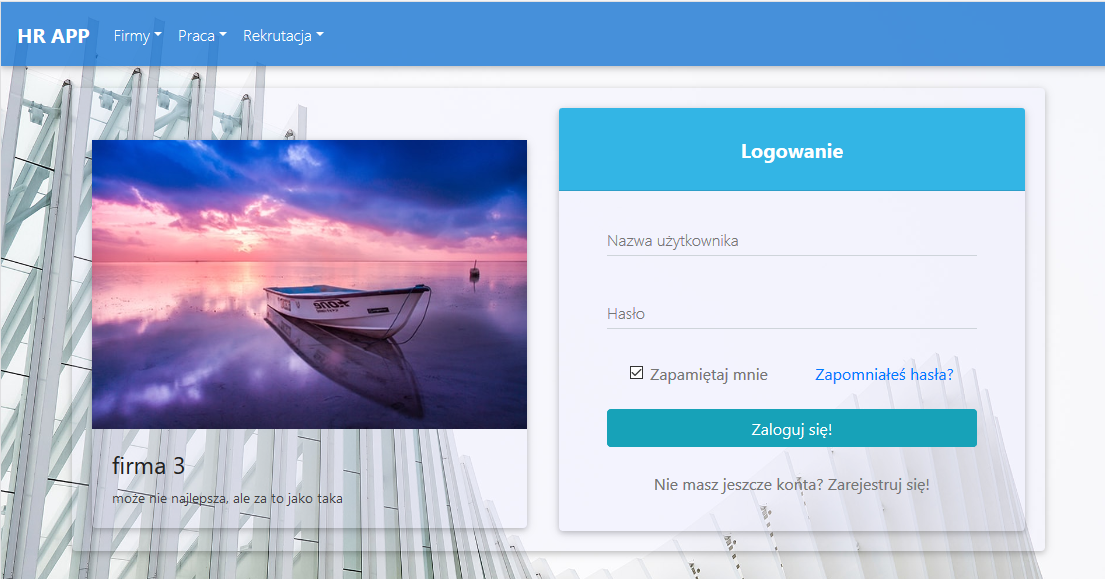
\includegraphics[width = \textwidth]{images/stronaGłówna.png}
    \caption{Strona główna. Źródło: Opracowanie własne.}
    \label{fig:strona_główna}
\end{figure}

Jako że jest to pierwsza wizyta, należy kliknąć w napis \textit{Nie masz jeszcze konta? Zarejestruj się!}, co zmieni widok na okno rejestracji.

\newpage

\begin{figure}[h!]
    \centering
    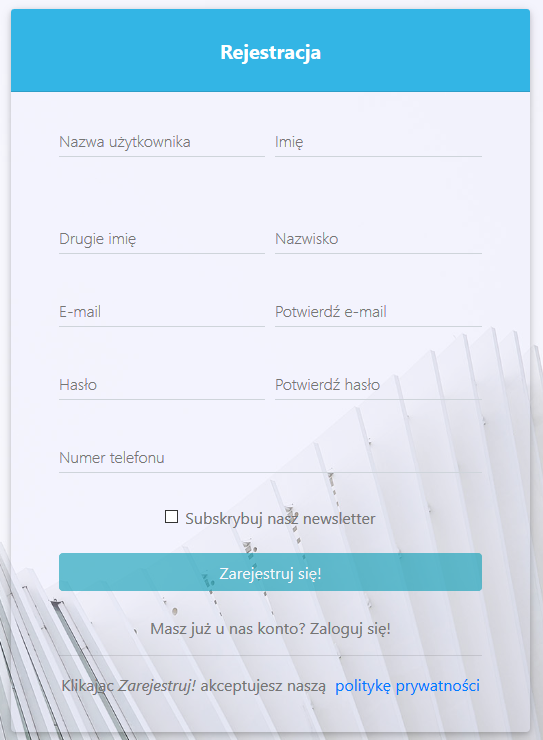
\includegraphics[scale=0.9]{images/rejestracja.png}
    \caption{Okno rejestracji. Źródło: Opracowanie własne.}
    \label{fig:okno_rejestracji}
\end{figure}

Oczywiście wszystkie pola przed wysłaniem są walidowane po stronie aplikacji internetowej. Jeśli któreś z nich nie spełnia jakiejś normy, to użytkownik zostanie poinformowany o tym, poprzez komunikat koloru czerwonego, pojawiający się pod nieprawidłowym polem.

\newpage

Po zarejestrowaniu i zalogowaniu, użytkownik zostaje przeniesiony na stronę główną, zawierającą komponent z prezentacją losowej firmy. Komponent ten, jest jedyną częścią wspólną dla wszystkich typów kont. Teraz w zależności, czy zalogowana jest osoba z kontem \textit{USER}, \textit{HR}, \textit{CEO} czy \textit{ADMIN}, taki widok i panele ma dostępne. \newline
\textbf{Interfejs zwykłego użytkownika:}

\begin{figure}[h!]
    \centering
    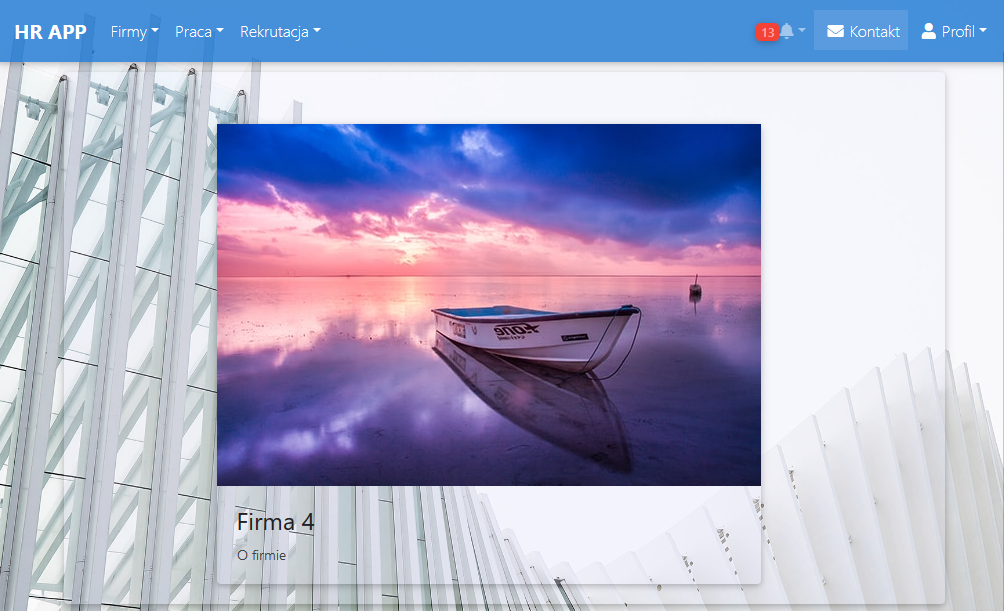
\includegraphics[width = \textwidth, scale=0.7]{images/stronaGłównaZalogowanyUser.png}
    \caption{Okno strony głównej użytkownika. Źródło: Opracowanie własne.}
    \label{fig:okno_strony_głównej_użytkownika}
\end{figure}

\newpage

\begin{figure}[h!]
    \centering
    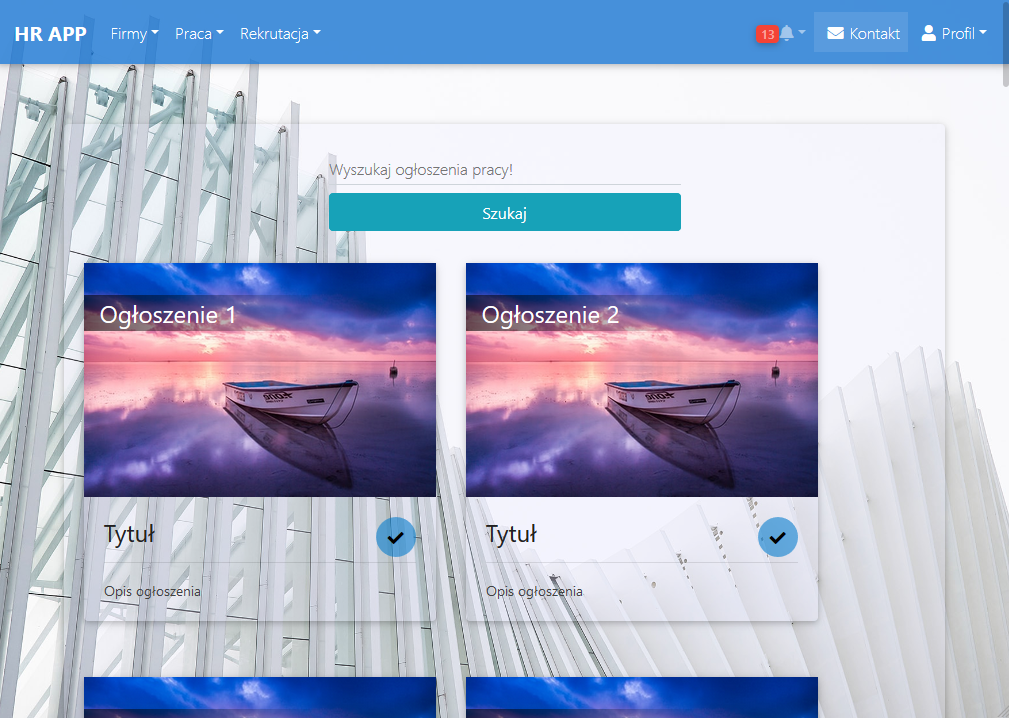
\includegraphics[width = \textwidth]{images/listaOgłoszeń.png}
    \caption{Okno listy ogłoszeń. Źródło: Opracowanie własne.}
    \label{fig:okno_listy_ogłoszeń}
\end{figure}

Duże karty stworzone w myśl zasad \textit{Material Design} czynią stronę przejrzystą i przyjazną dla urządzeń z mniejszymi ekranami.

\begin{figure}[h!]
    \centering
    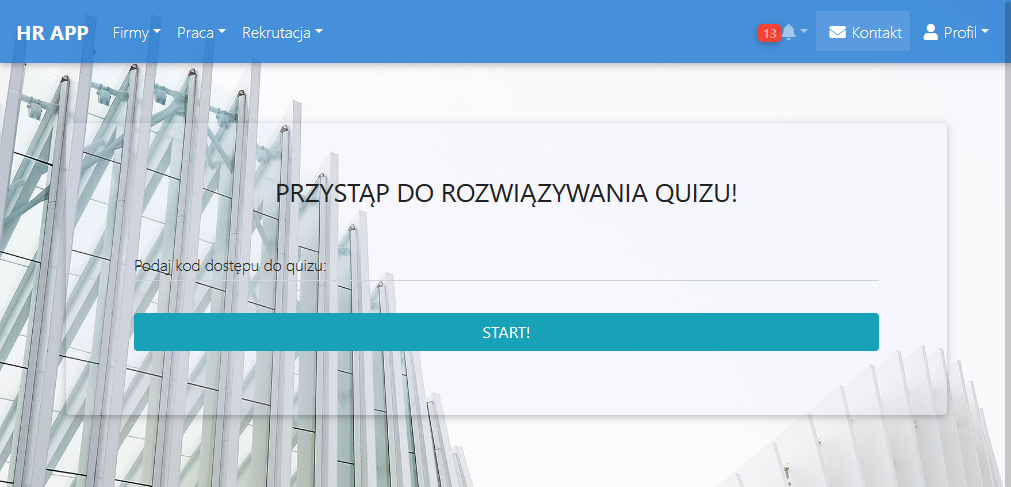
\includegraphics[width = \textwidth]{images/panelQuizu2.png}
    \caption{Okno wyboru testu. Źródło: Opracowanie własne.}
    \label{fig:okno_wyboru_testu}
\end{figure}

\newpage

\begin{figure}[h!]
    \centering
    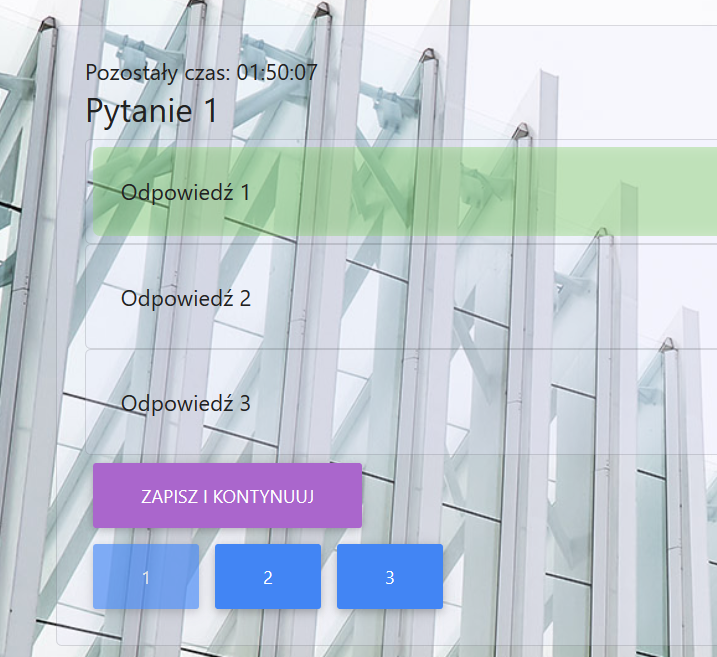
\includegraphics[width = \textwidth]{images/rozwiązywanieQuizu.png}
    \caption{Okno rozwiązywania testu. Źródło: Opracowanie własne.}
    \label{fig:okno_rozwiązywania_testu}
\end{figure}

Panel rozwiązywania testu (rysunek \ref{fig:okno_rozwiązywania_testu}) posiada prosty, duży i przejrzysty interfejs, dzięki czemu osoba odpowiadająca na pytania może się skupić na nich samych, zamiast na obsłudze aplikacji.

\newpage

\begin{figure}[h!]
    \centering
    
\includegraphics[width = \textwidth]{images/powiadomienie.png}
    \caption{Rozwinięcie ikonki powiadomień. Kliknięcie w tekst spowoduje przeniesienie do listy aplikacji użytkownika. Źródło: Opracowanie własne.}
    \label{fig:ikonka_powiadomień_użytkownika_rozwinięta}
\end{figure}

\begin{figure}[h!]
    \centering
    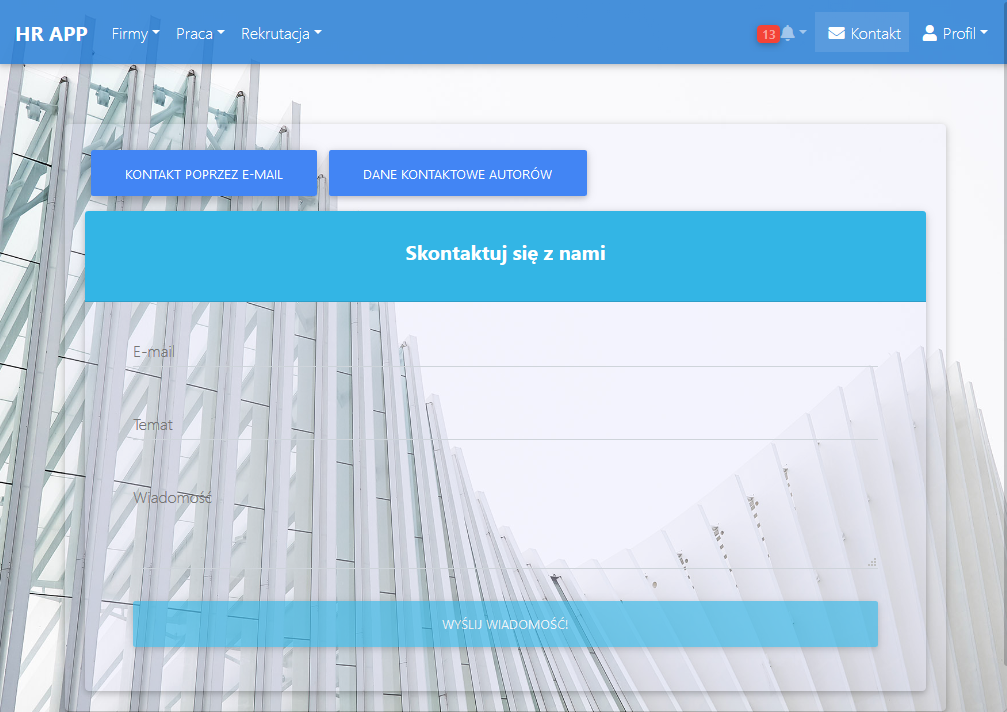
\includegraphics[width = \textwidth]{images/oknoKontaktuEmail.png}
    \caption{Okno kontaktu e-mail. Źródło: Opracowanie własne.}
    \label{fig:okno_kontaktu_email}
\end{figure}

Dzięki zastosowaniu obsługi poczty na części serwerowej, został udostępniony formularz kontaktowy dla wszystkich tych, którzy chcieliby podzielić się czymś\linebreak z administratorami strony.

\newpage

\begin{figure}[h!]
    \centering
    
\includegraphics[scale=0.7]{images/rozwinięcieProfilu.png}
    \caption{Rozwinięcie menu profilu. Źródło: Opracowanie własne.}
    \label{fig:rozwinięcie_profilu}
\end{figure}

\begin{figure}[h!]
    \centering
    
\includegraphics[width = \textwidth]{images/mojeKonto.png}
    \caption{Okno moje konto. Źródło: Opracowanie własne.}
    \label{fig:okno_moje_konto}
\end{figure}

Pod zakładką moje konto znajdziemy szereg przycisków zajmujących się obsługą profilu (rysunek \ref{fig:okno_moje_konto}). Rysunki \ref{fig:okno_zmiany_hasła}, \ref{fig:okno_subskrypcji_email} oraz \ref{fig:okno_przesyłania_cv} przedstawiają rozwinięcie wybranych opcji.

\newpage

\begin{figure}[h!]
    \centering
    \includegraphics[width = \textwidth]{images/zmianaHasła.png}
    \caption{Okno zmiany hasła. Źródło: Opracowanie własne.}
    \label{fig:okno_zmiany_hasła}
\end{figure}

Na rysunku \ref{fig:okno_zmiany_hasła} widać rozwiniętą opcję zmiany hasła. Każda zmiana jakichkolwiek danych konta, musi być potwierdzona poprzez podanie aktualnego hasła. Przycisk wyślij jest nieaktywny do momentu poprawnego uzupełnienia formularza (jest on także walidowany). Komponenty do zmiany numeru telefonu i adresu e-mail wyglądają identycznie i różnią się tylko odpowiednimi polami. 

\begin{figure}[h!]
    \centering
    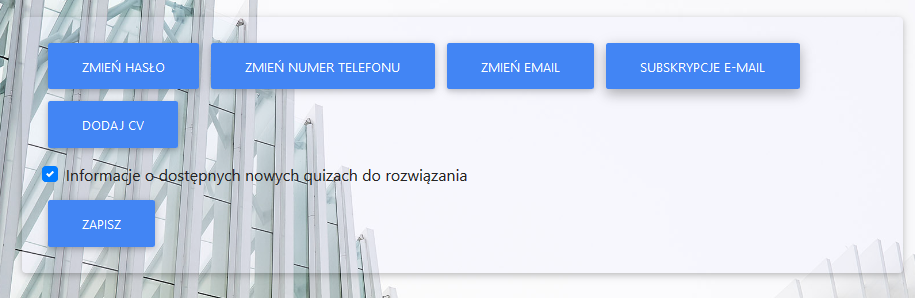
\includegraphics[width = \textwidth]{images/subskrypcjaEmail.png}
    \caption{Okno subskrypcji e-mail. Źródło: Opracowanie własne.}
    \label{fig:okno_subskrypcji_email}
\end{figure}

\newpage

\begin{figure}[h!]
    \centering
    \includegraphics[width = \textwidth]{images/przesyłCv.png}
    \caption{Okno przesyłania \textit{CV}. Źródło: Opracowanie własne.}
    \label{fig:okno_przesyłania_cv}
\end{figure}

\begin{figure}[h!]
    \centering
    
\includegraphics[width = \textwidth]{images/ustawienia.png}
    \caption{Okno ustawień. Źródło: Opracowanie własne.}
    \label{fig:okno_ustawień}
\end{figure}

Jako, że aplikacja jest przewidziana dla wielu narodowości, tak też zostały udostępnione dwie opcje językowe do wyboru. Dzięki niezaszywaniu tekstów w znacznikach HTML, a korzystaniu z usługi tłumaczącej, która wstawia w odpowiednie miejsca odpowiednią wersję językową.

\newpage

\textbf{Interfejs użytkownika HR:}
\begin{figure}[h!]
    \centering
    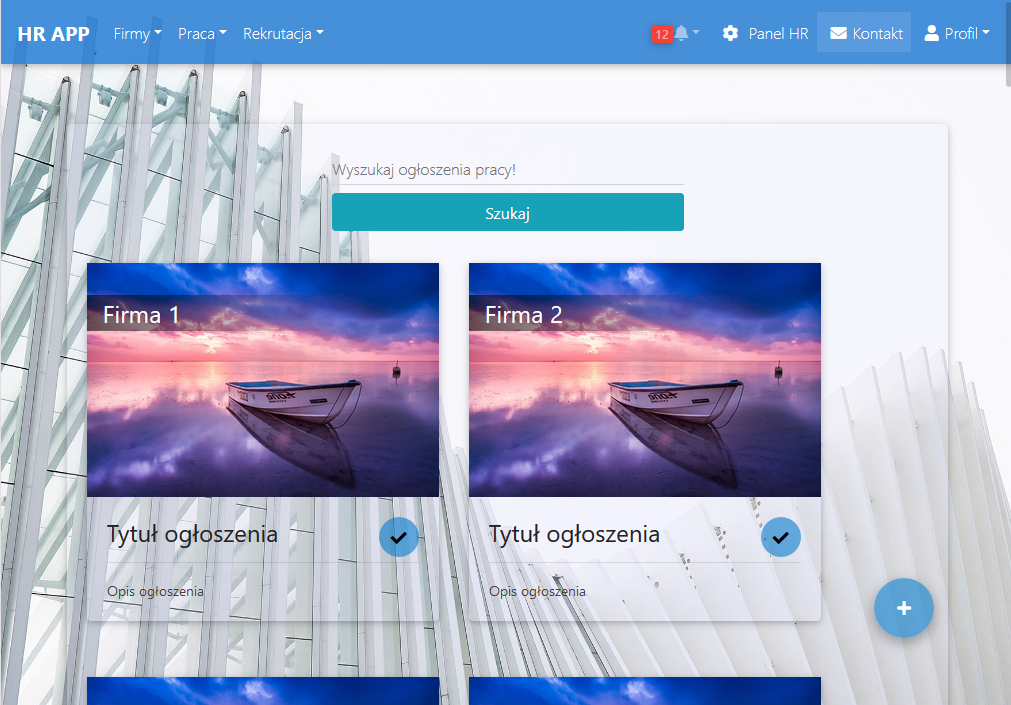
\includegraphics[scale=0.5]{images/listaOgłoszeńHR.png}
    \caption{Okno listy ogłoszeń, u użytkownika \textit{HR} różni się lewitującym przyciskiem w prawej dolnej części ekranu, który przenosi do widoku tworzenia nowego ogłoszenia. Źródło: Opracowanie własne.}
    \label{fig:lista_ogłoszeń_hr}
\end{figure}

\newpage

\begin{figure}[h!]
    \centering
    
\includegraphics[width = \textwidth]{images/dodawanieOgłoszeńPracy.png}
    \caption{Widok tworzenia nowego ogłoszenia. Źródło: Opracowanie własne.}
    \label{fig:okno_tworzenia_ogłoszenia_pracy}
\end{figure}

\begin{figure}[h!]
    \centering
    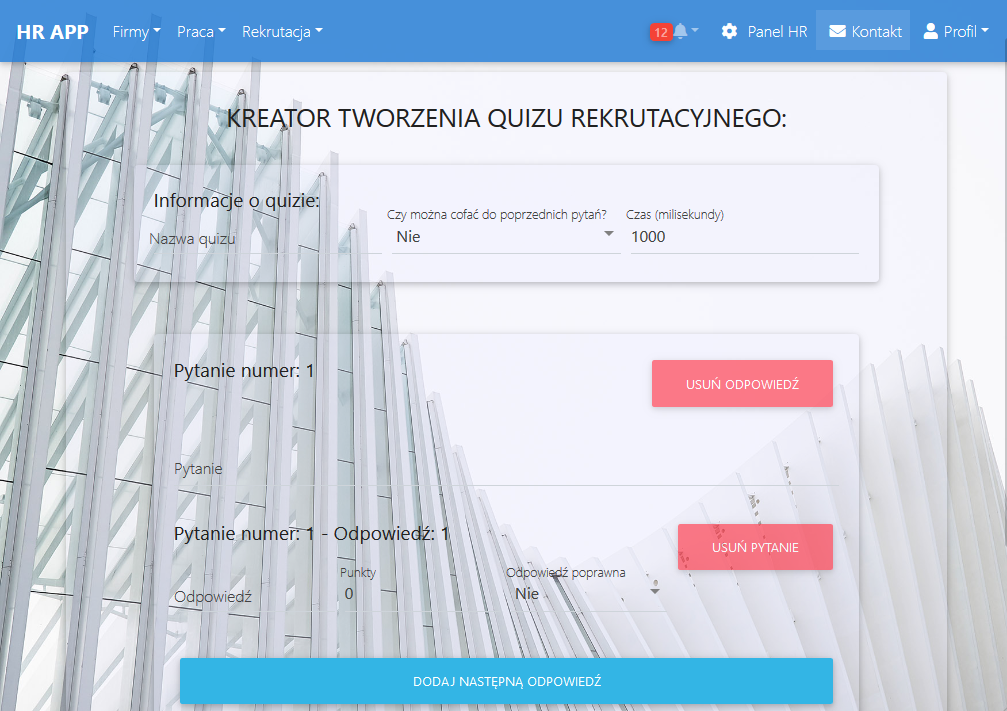
\includegraphics[scale=0.5]{images/kreatorTworzeniaQuizu.png}
    \caption{Tworzenie nowego testu rekrutacyjnego. Źródło: Opracowanie własne.}
    \label{fig:okno_tworzenia_testu_rekrutacyjnego}
\end{figure}

Jeśli nastałaby sytuacja, że podczas tworzenia nowego testu rekrutacyjnego, zostanie przerwane połączenie z internetem, bądź wystąpi jakakolwiek inna sytuacja, która spowoduje konieczność przerwania prac nad kreatorem, tym samym nie ukańczając całego procesu, to nic straconego. Wersja robocza testu zostaje zapisywana do pamięci podręcznej przeglądarki i podczas powrotu do okna kreacji, zostaniemy poinformowani o tym fakcie i zapytani czy chcemy wczytać zapisany stan. Rysunek z tym komunikatem jest przedstawiony w rozdziale 8.2.2.

\begin{figure}[h!]
    \centering
    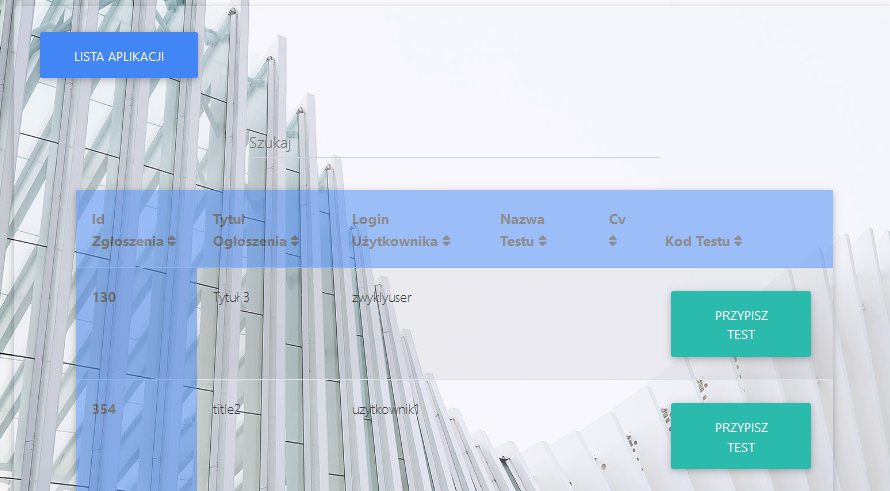
\includegraphics[scale=0.6]{images/listaAplikacjiHr.png}
    \caption{Widok listy aplikacji złożonych przez użytkowników. Źródło: Opracowanie własne.}
    \label{fig:lista_aplikacji_hr}
\end{figure}

\begin{figure}[h!]
    \centering
    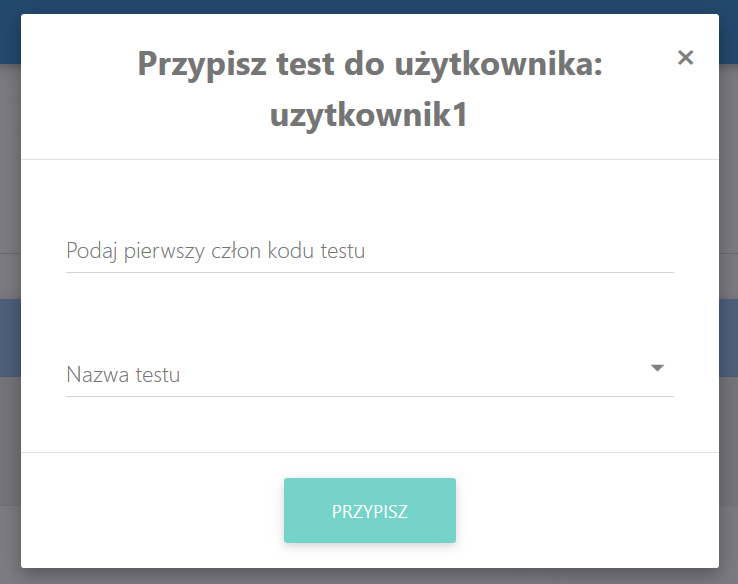
\includegraphics[scale=0.4]{images/modalPrzypisywaniaTestu.png}
    \caption{Okno przypisywania testu do użytkownika. Źródło: Opracowanie własne.}
    \label{fig:okno_przypisywania_testu_rekrutacyjnego}
\end{figure}

\newpage

\textbf{Interfejs użytkownika CEO:}

\begin{figure}[h!]
    \centering
    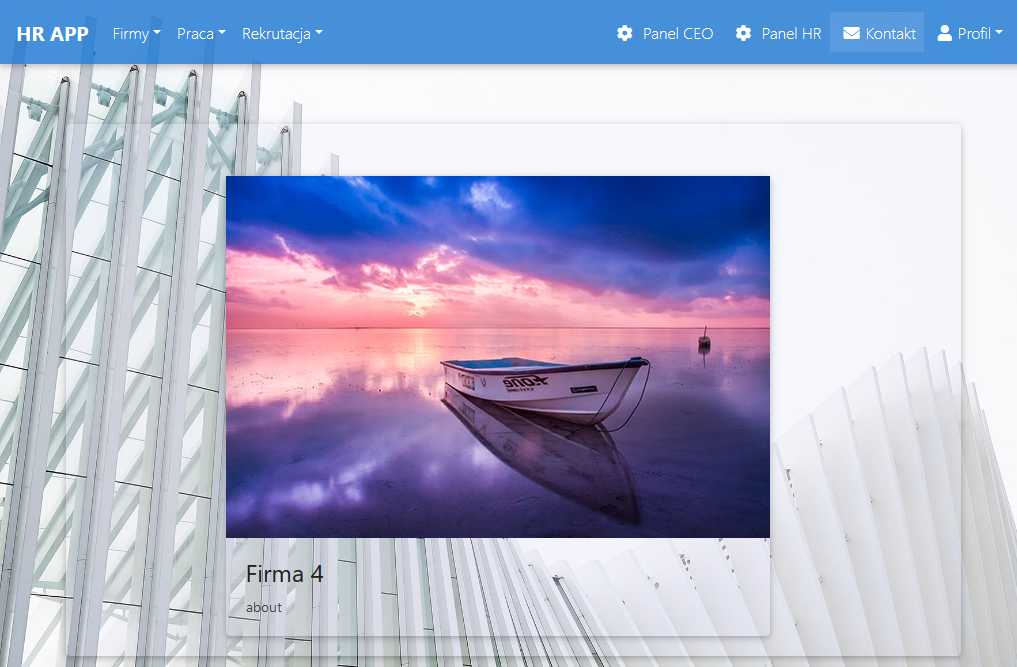
\includegraphics[scale=0.6]{images/stronaGłównaCeo.png}
    \caption{Okno strony głównej użytkownika \textit{CEO}. Źródło: Opracowanie własne.}
    \label{fig:strona_główna_CEO}
\end{figure}

Jednymi z funkcjonalności dostępnych tylko dla użytkownika \textit{CEO} jest przypisywanie nowych i kasowanie obecnych użytkowników \textit{HR}. Okno ich wyboru zostało przedstawione na rysunku \ref{fig:panel_ceo}.

\begin{figure}[h!]
    \centering
    
\includegraphics[width = \textwidth]{images/panelCeo.png}
    \caption{Panel użytkownika \textit{CEO}. Źródło: Opracowanie własne.}
    \label{fig:panel_ceo}
\end{figure}

\newpage

\begin{figure}[h!]
    \centering
    
\includegraphics[width = \textwidth]{images/rejestracjaFirmy.png}
    \caption{Okno rejestracji firmy. Źródło: Opracowanie własne.}
    \label{fig:okno_rejestracji_firmy}
\end{figure}

\begin{figure}[h!]
    \centering
    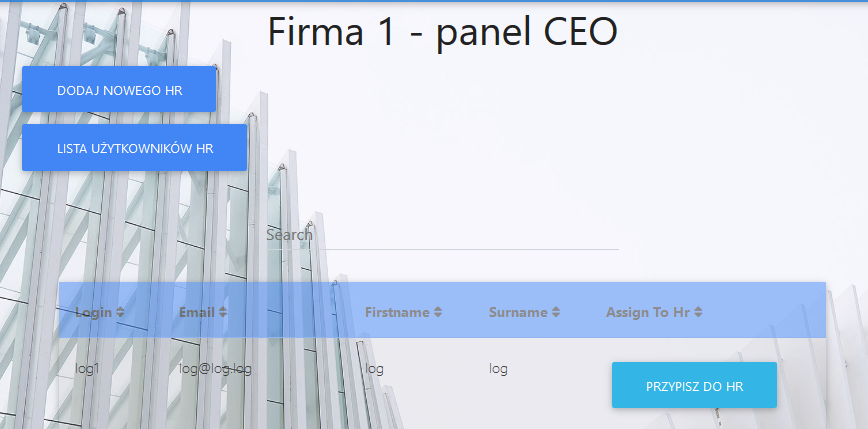
\includegraphics[width = \textwidth]{images/dodawanieHr.png}
    \caption{Fragment tabeli dodawania użytkownika \textit{HR} do firmy. Źródło: Opracowanie własne.}
    \label{fig:panel_dodawania_hr}
\end{figure}

\newpage

\begin{figure}[h!]
    \centering
    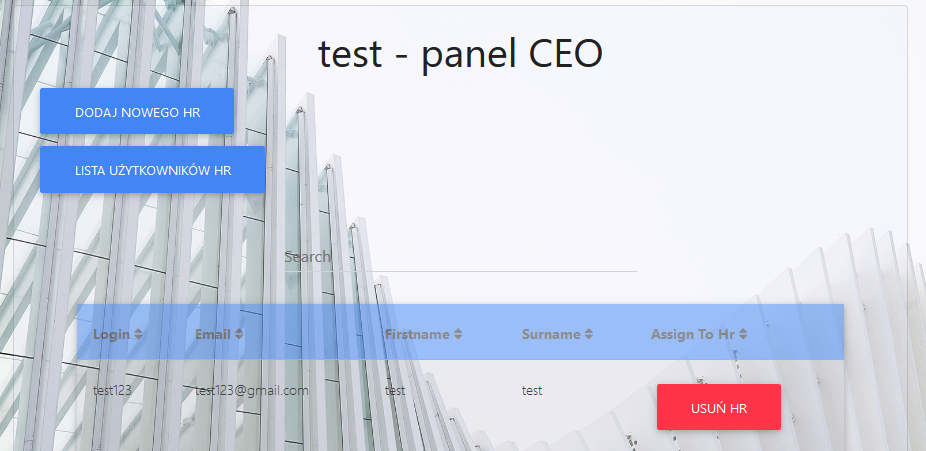
\includegraphics[width = \textwidth]{images/kasowanieHr.png}
    \caption{Fragment tabeli wykluczania użytkownika \textit{HR} z firmy. Źródło: Opracowanie własne.}
    \label{fig:panel_kasowania_hr}
\end{figure}

\textbf{Interfejs użytkownika ADMIN.}

\begin{figure}[h!]
    \centering
    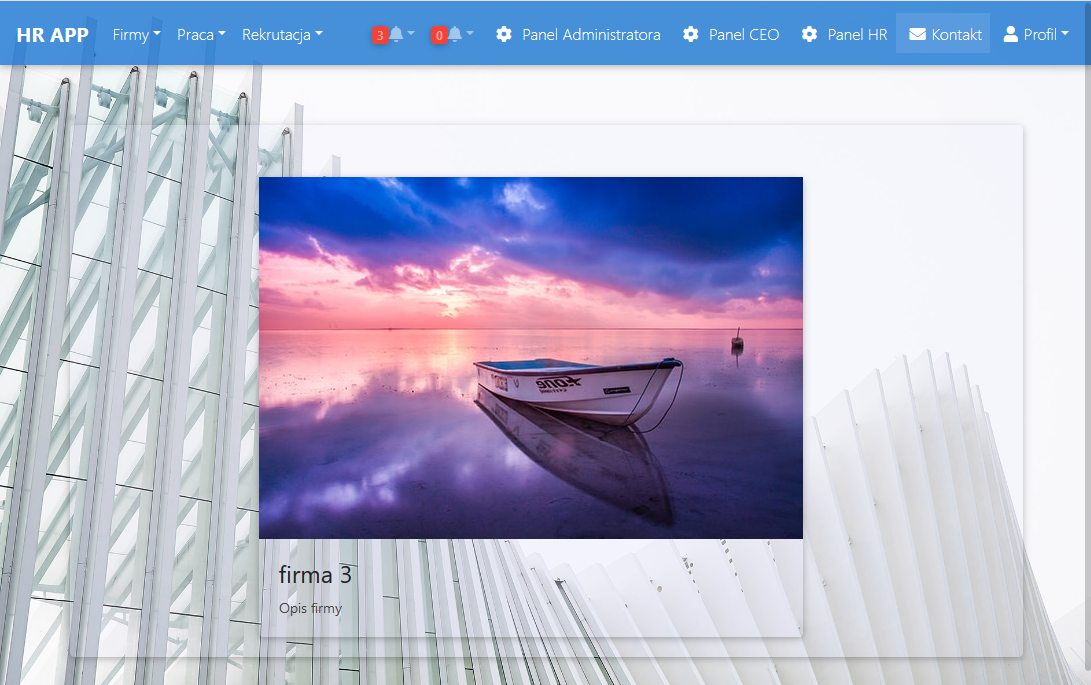
\includegraphics[width = \textwidth]{images/stronaGłównaAdmin.png}
    \caption{Okno strony głównej administratora. Źródło: Opracowanie własne.}
    \label{fig:strona_główna_admin}
\end{figure}

\newpage

\begin{figure}[h!]
    \centering
    
\includegraphics[width = \textwidth]{images/panelAdmin.png}
    \caption{Panel administratora. Źródło: Opracowanie własne.}
    \label{fig:panel_administratora}
\end{figure}

\begin{figure}[h!]
    \centering
    
\includegraphics[width = \textwidth]{images/dodawanieTypuKonta.png}
    \caption{Panel dodawania typu konta. Źródło: Opracowanie własne.}
    \label{fig:dodawanie_typu_konta}
\end{figure}

Jako, że projekt jest wysoce przygotowany na zmiany i rozbudowę, zespół projektowy przygotował pole, gdzie administrator może dodać kolejne typy kont, jeśli tylko najdzie taka potrzeba.

\begin{figure}[h!]
    \centering
    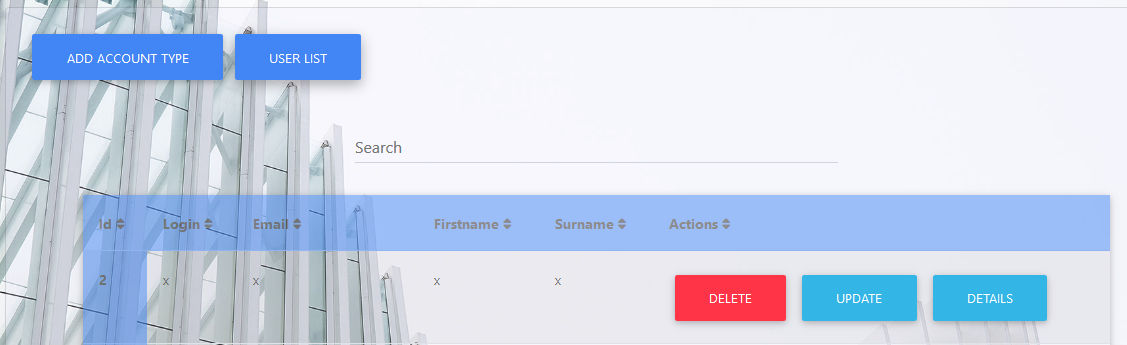
\includegraphics[width = \textwidth]{images/listaUżytkowników.png}
    \caption{Fragment listy użytkowników. Źródło: Opracowanie własne.}
    \label{fig:lista_użytkowników}
\end{figure}

\newpage

\begin{figure}[h!]
    \centering
    \includegraphics[scale=0.6]{images/oknoEdycjiUżytkownika.png}
    \caption{Okno edycji użytkownika. Źródło: Opracowanie własne.}
    \label{fig:edycja_użytkownika}
\end{figure}

Administrator jako jedyny ma możliwość pełnej edycji danych użytkownika.

\begin{figure}[h!]
    \centering
    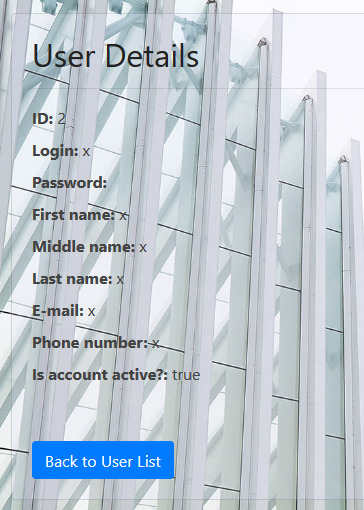
\includegraphics[scale=0.6]{images/szczegółyUżytkownika.png}
    \caption{Okno szczegółów użytkownika. Źródło: Opracowanie własne.}
    \label{fig:szczegóły_użytkownika}
\end{figure}

\newpage

Oczywiście strona jest w pełni responsywna i jej wygląd zmienia się wraz\linebreak z rozdzielczością ekranu, na którym ją przeglądamy.
\subsubsection{Biblioteki}
\begin{itemize}
    \item \textbf{chart.js}\newline
    Biblioteka została zaimportowana na wypadek, gdyby w aplikacji była konieczność wdrożenia wykresów np. dla statystyk użytkowników, czy testów.
    \item \textbf{crypto-js}\newline
    Pozwala na szyfrowanie danych. Została wykorzystana podczas zapisywania danych o tworzonym teście do \textit{localStorage}. Zapewnia to bezpieczne przechowywanie danych o rozpoczętym tworzonym teście, ale jeszcze nie zapisanym do bazy. Takie rozwiązanie zostało zaimplementowane, by twórca testu nie musiał od razu go zapisywać, tylko -- by do momentu zatwierdzenia -- przetrzymywany był lokalnie. Zaszyfrowanie zawartości \textit{JSON} zabezpiecza przed podejrzeniem \textit{localStorage} przed osobami niepowołanymi.

\item \textbf{flag-icon-css}\newline
Mała biblioteka, pozwalająca na insercję do pliku \textit{HTML} ikonki flagi. Wykorzystana przy wyborze języka aplikacji.

\begin{lstlisting}[language=html,caption=Implementacja ikonki flagi. Źródło: Opracowanie własne.,captionpos=b]
<span 
 class="flag-icon flag-icon-{{language|transformFlag}}">
</span>
\end{lstlisting}
Gdzie \textit{\{\{language $|$ transformFlag\}\}} to skrócona nazwa języka, np. \textit{pl}, \textit{en}.

\item \textbf{jwt-decode}\newline
Pozwala na dekodowanie tokenów \textit{JWT}. Dzięki tej bibliotece, można skorzystać z przysłaniania przycisków, miejsc w aplikacji, do których użytkownik nie ma dostępu, ponieważ nie ma przydzielonych uprawnień do tych zasobów.\newline
\newpage
\begin{lstlisting}[language=Java,caption=Implementacja sprawdzenia poprawności tokenu oraz jego ważności. Źródło: Opracowanie własne.,captionpos=b]
  public isAuthenticated(): boolean {
    const jwtHelper = new JwtHelperService();
    const token = localStorage.getItem(TOKEN_KEY);

    return !this.jwtHelper.isTokenExpired(token);
  }
\end{lstlisting}

\begin{lstlisting}[language=Java,caption=Pobranie nazwy użytkownika i przypisanej roli do localStorage. Źródło: Opracowanie własne.,captionpos=b]
  public saveUserInLocalStorage(token) {
    if (token) {
      const decodedToken = decode(token);
      this.saveToken(token);
      this.saveUser(decodedToken.sub);
      this.saveRole(decodedToken.role);
    }
  }
\end{lstlisting}
Poza zabezpieczeniem od strony klienckiej, również serwer jest zabezpieczony przed niepowołanym dostępem do zasobów. Jeżeli użytkownik, pomimo braku uprawnień, spróbuje odpytać punkt końcowy, do którego nie ma dostępu, nie uzyska odpowiedzi.

\item \textbf{mdbootstrap}\newline
Biblioteka, która wspiera szybkie tworzenie stron internetowych, za pomocą wbudowanych stylów. W projekcie została wykorzystana darmowa, ograniczona wersja.

\item \textbf{ngx-toastr}\newline
Paczka, która pozwala na implementację małych powiadomień po wykonaniu akcji. W projekcie powiadomienia pokazują się np. podczas wystąpienia błędu po stronie serwera, po poprawnym dodaniu testu itp.

    \begin{figure}[h!]
        \centering
        
\includegraphics[scale=0.8]{images/toastError.JPG}
        \caption{Komunikat błędu. Źródło: Opracowanie własne.}
        \label{fig:toast_error}
    \end{figure}
    
\item \textbf{rxjs}\newline
Biblioteka została wykorzystana w celu obsługi zapytań serwera. Szerzej opisana została w rozdziale \textbf{8.2.11}.

\item \textbf{sweetalert2}\newline
Dodatek, który pozwala na tworzenie wyskakujących okienek, z którym użytkownik może wchodzić w interakcję. Został wykorzystany np. w pytaniu\linebreak o potwierdzenie, czy użytkownik chce wczytać poprzednio tworzony test, czy rozpocząć tworzenie nowego.

    \begin{figure}[h!]
        \centering
        \includegraphics[scale=0.9]{images/sweetalert.JPG}
        \caption{Pytanie stworzone za pomocą \textit{SweetAlert2}. Źródło: Opracowanie własne.}
        \label{fig:sweetalert}
    \end{figure}

\end{itemize}

\subsubsection{Budowa projektu }
Budowa projektu zostanie omówiona z pominięciem podstawowych plików, generowanych przy każdej aplikacji, wytworzonej w środowisku programistycznym \textit{Angular}.
Uproszczone drzewo plików:
\newpage
\begin{lstlisting}[caption=Uproszczone drzewo plików aplikacji internetowej. Źródło: Opracowanie własne.,captionpos=b]
>src
    >app
        >classes
        >common
        >components
            >navbar
                -navbar.component.html
                -navbar.component.scss
                -navbar.component.ts
            >panels
                >user-panel
                    >user-list-of-applications
                        -user-list-of-applications
                        .component.html
                        -user-list-of-applications
                        .component.scss
                        -user-list-of-applications
                        .component.ts    
                    -user-panel.component.html
                    -user-panel.component.scss
                    -user-panel.component.ts
            ...
        >factories
        >helpers
        >modules
        >pipes
        >services
            >security
                -auth-guard.service.ts
                ...
            -mailing.service.ts
            ...
        -app.component.html
        -pp.component.scss
        -app.component.ts
    >assets
    >environments
\end{lstlisting}


W głównym folderze \textit{src}, znajduje się kod źródłowy, rozmieszczony po różnych podfolderach. Znajdują się w nim również: plik odpowiedzialny za trasowanie stron oraz najważniejsze cztery pliki, czyli:  \textit{app.component.html},  \textit{app.component.scss}, \linebreak \textit{app.component.ts} oraz \textit{app.module.ts}, czyli składowe głównej strony.

W katalogu \textit{classes} znajdują się pliki \textit{TypeScript}, określające klasy danych, później używanych w kodzie. Jest tam między innymi definicja klasy użytkownika\linebreak w pliku \textit{user.ts}.

W lokacji \textit{common} został umieszczony plik \textit{global\-constants.ts}, w którym są stałe globalne, takie jak adres serwera, czy opcje \textit{http} potrzebne do generowania zapytań.

Największym z podfolderów jest \textit{components}. Jak sama nazwa wskazuje, znajdują się tam wszystkie komponenty (które także są umieszczone we własnych podfolderach) użyte do budowy aplikacji. Można tam znaleźć takie elementy, jak: wszystkie panele użytkowników, pasek nawigacji, czy stronę edycji danych konta.

Kolejną, pomniejszą lokacją, jest \textit{factories}, która przewidziana jest na fabryki. Znajduje się tam tylko jeden plik \textit{appInitializerFactory.ts}, którego zadaniem jest implementacja działania usługi językowej aplikacji.

Folder \textit{helpers} z założenia ma zawierać pliki, ułatwiające walidację formularzy. Znajduje się tam plik \textit{must-match.ts}, który porównuje dwa przekazane mu argumenty, czy są identyczne. Jest używany między innymi do walidacji adresu e-mail przy zakładaniu konta.

Katalog \textit{modules} przewidziany jest na przechowywanie modułów. W projekcie znalazł tam miejsce moduł \textit{pipes.module.ts}, który jest używany między innymi\linebreak do tłumaczeń tekstu w plikach \textit{HTML}.

W lokacji \textit{pipes} jest miejsce na funkcje bezpośredniego przekształcania. Znajduje się tam plik \textit{transform-flag.pipe.ts}, który jest odpowiedzialny za dostosowanie flagi przypisanej do języka wybranej nacji.

\textit{Services} to druga większa lokacja, skupiająca serwisy. Znajduje się w niej tylko jeden podfolder \textit{security}, w którym skatalogowane są pliki odpowiedzialne za kontrolę dostępu, autoryzację, szyfrowanie i obsługę tokenów. 

\subsubsection{HTTP interceptors}
Interceptory służą do przechwytywania zapytań \textit{http} i ich modyfikacji. W \textit{Angularze} zostały zaimplementowane narzędzia do ich obsługi, które zapewniają ich prawidłowe działanie. Poprzez interceptory możemy przechwycić każde wywołanie \textit{http} od strony klienckiej oraz zmodyfikować jego zawartość, po czym przekazać zapytanie dalej, do obsługi wewnątrz aplikacji. Można również przy pomocy interceptorów wykonywać operacje w drugą stronę, tzn. przechwytywać odpowiedzi z serwera,\linebreak a następnie wykonywać na nich dowolne operacje.
Aby poinformować aplikację\linebreak o chęci korzystania z interceptorów, należy w module (najlepiej głównym) zaimportować interceptory.
\begin{lstlisting}[language=Java,caption=Przykład importowania interceptorów. Źródło: Opracowanie własne.,captionpos=b]
    import { http_INTERCEPTORS } from '@angular/common/http';
\end{lstlisting}
Następnie należy poinformować moduł aplikacji o tym, która klasa będzie miała możliwość edycji zapytań.
\begin{lstlisting}[language=Java,caption=Poinformowanie aplikacji o możliwości edycji zapytań. Źródło: Opracowanie własne.,captionpos=b]
    providers[
    ...
        {
          provide: http_INTERCEPTORS,
          useClass: TokenInterceptor,
          multi: true,
        }
    ...
    ]
\end{lstlisting}
W przypadku tej aplikacji, głównym zadaniem interceptorów jest doczepianie \textit{Bearer tokenu} do nagłówka zapytania. Token otrzymywany jest po udanej próbie zalogowania. Pobierany jest z lokalnych zasobów przeglądarki predefiniowanych dla wybranego adresu (ang. \textit{local storage}). Oprócz tego, dodatkowo doczepiana jest informacja o typie \textit{MIME} (ang. \textit{Multipurpose Internet Mail Extensions}), czyli rodzaju wysyłanego pliku poprzez zapytanie. W przypadku tej aplikacji, w większości konstruowane są zapytania w formacie \textit{JSON}.\newline

\subsubsection{Przechowywanie informacji}
W aplikacji internetowej wykorzystywana jest pamięć lokalna (ang. \textit{local storage}). Są w niej przechowywane takie dane, jak:
\begin{itemize}
    \item auth-role -- typ zalogowanego konta,
    \item auth-token -- token uwierzytelniający użytkownika,
    \item auth-user -- login użytkownika,
    \item lang -- język interfejsu aplikacji,
    \item quiz-create-panel-data -- dane zapisane z nieukończonego procesu tworzenia nowego testu.
\end{itemize}

\begin{figure}[h!]
    \centering
    \includegraphics[scale=0.9]{images/token.png}
    \caption{Przykładowe dane przechowywane w pamięci lokalnej. Źródło: Opracowanie własne.}
    \label{fig:token}
\end{figure}

\subsubsection{Wykorzystane szyfrowanie}
W części webowej aplikacji, szyfrowanie zostało użyte do przetrzymywania\linebreak w \textit{local storage} informacji o tworzonym teście -- tak, by móc wrócić do jego tworzenia w przyszłości. W tym cel została wykorzystana biblioteka \textit{crypto-js}. W projekcie wykorzystano szyfrowanie za pomocą \textit{AES} (\textit{Advanced Encryption Standard}), czyli symetrycznego szyfru blokowego. \textit{AES} wykorzystuje sieć substytucji i permutację macierzową. Do szyfrowania i deszyfrowania danych, wykorzystywany jest zdefiniowany, sekretny klucz o długości 128, 192 lub 256 bitów. Im dłuższy klucz, tym większa jest liczba rund szyfrujących\footnote{Materiały serwisu Crypto-IT, \url{http://www.crypto-it.net/pl/symetryczne/aes.html},\newline (dostęp 14.12.2020)}. \newline
W procesie szyfrowania tekst jawny dzielony jest na bloki 128-bitowe. Bloki tworzone są jako macierze $4x4$:
$$\left[\begin{array}{cccc}
b_{0}&b_{4}&b_{8}&b_{12}\\
b_{1}&b_{5}&b_{9}&b_{13}\\
b_{2}&b_{6}&b_{10}&b_{14}\\
b_{3}&b_{7}&b_{11}&b_{15}\\
\end{array}\right]$$
Dla każdej z macierzy wykonywane są następujące operacje:
\begin{itemize}
    \item Przygotowanie podkluczy\newline
    Następuje wygenerowanie jednego podklucza początkowego, a następnie po jednym kluczu dla każdej z rund szyfrujących.
    \item Runda inicjująca\newline
    Na każdym bajcie w bloku danych wykonywana jest operacja sumowania \textit{XOR}, z odpowiadającym mu pierwszym podkluczem.
    \item $n$ rund szyfrujących\newline
    Gdzie $n$ dla klucza 128-bitowego wynosi 9, dla klucza 192-bitowego – 11, natomiast dla 265-bitowego – 13.\newline
    Każda runda szyfrująca składa się z następujących operacji:
    \begin{itemize}
        \item Zastępowanie każdego bajtu innym bajtem — wykorzystuje się do tego tzw. \textit{S-Box'y Rijndael'a}.
        \item Przesunięcie bajtów w trzech ostatnich macierzach stanu w lewo.
\[
\begin{bmatrix}
b_{0}&b_{4}&b_{8}&b_{12}\\
b_{1}&b_{5}&b_{9}&b_{13}\\
b_{2}&b_{6}&b_{10}&b_{14}\\
b_{3}&b_{7}&b_{11}&b_{15}\\     
\end{bmatrix}
\to
\begin{bmatrix}
b_{4}&b_{8}&b_{12}&b_{0}\\
b_{5}&b_{9}&b_{13}&b_{1}\\
b_{6}&b_{10}&b_{14}&b_{2}\\
b_{7}&b_{11}&b_{15}&b_{3}\\   
\end{bmatrix} 
\]
        \item Mnożenie kolumn — każda z kolumn w macierzach stanu jest przemnażana przez macierz $4x4$ bajtów.
        \item Działanie \textit{XOR} na wszystkich bajtach bloku danych i bajtach podklucza danej rundy.
    \end{itemize}
    \item Runda kończąca\newline
    Wykonywane są wszystkie operacje z rundy szyfrującej, poza operacją mnożenia kolumn.
\end{itemize}
Przykładowy wynik szyfrowania ciągu znaków zbudowanego z obiektu \textit{JSON}, który przechowywał strukturę tworzonego testu:
\begin{lstlisting}[caption=Zaszyfrowany obiekt JSON przechowujący strukturę tworzonego testu. Źródło: Opracowanie własne., captionpos=b]
    U2FsdGVkX1+AtQ8Tg2ru29Lfw7Ub0qK4jNwQw1B+RNFdKAO3nF/9K/ge
    8yyv0pleYsqVyDkJjKaWQQ72huq7eYy7dKaES+JhjrfsDxhyyxHEltAT
    ad8vJHBcarNckEXhXk4ySohvnoQZRRDO2WM5TQ0a9+esoHVrOXNcsyhm
    oyGX/cEIFOt78cBpKkpKCX7+GZQphyQPSZ3owusSlOb950XslpNnDyOA
    RS+Wx/V3T92RLEdP+nrVnqFdSxwafjreiieih4dqxyvY/BCWzQT9tLpV
    3W4la6ZLmixjlh95Kww7jUpS1L8i4NV7cE1Mhd1NsTx4l4Tr4P2iV2Ue
    KR3a3aZ7YsMYhwBNOlQ0nOv7Y2Lxj+6Vood5OWWOtKXdLXiniIJ4l3iQ
    d3x8jGyijrhTSAQFXGOlFU2qDsRPWsHNwCb9hMjjHETQsQvR9I8VE1S
\end{lstlisting}

\begin{lstlisting}[language=Java,caption=Implementacja szyfrowania i deszyfrowania poprzez AES wykorzystując wygenerowany sekretny klucz. Źródło: Opracowanie własne., captionpos=b]
import { Injectable } from '@angular/core';
import * as CryptoJS from 'crypto-js';

@Injectable({
  providedIn: 'root'
})
export class CryptoService {

  encryptSecretKey = 'ca17828f861a0a6c7cc70586af2e0ee1';

  constructor() { }

  encryptData(data) {
    try {
      return CryptoJS.AES.encrypt(JSON.stringify(data)
      , this.encryptSecretKey).toString();
    } catch (e) {
      return null;
    }
  }

  decryptData(data) {
    try {
      const bytes = CryptoJS.AES.decrypt(data, 
                        this.encryptSecretKey);
      if (bytes.toString()) {
        return JSON.parse(bytes.toString(CryptoJS
            .enc.Utf8));
      }
      return data;
    } catch (e) {
      return null;
    }
  }
}
\end{lstlisting}

\subsubsection{Angular Hooks}
Każdy komponent i dyrektywa (ang. \textit{directive}) w \textit{Angularze} posiada swój cykl życia. Aby mieć jak największą kontrolę nad aplikacją, należy się w jakiś sposób podpiąć pod te cykle. Można to zrobić właśnie za pomocą haków cyklu życia komponentu (ang. \textit{lifecycle hooks}). Wywołują się one w takiej kolejności:
\begin{itemize}
    \item constructor,
    \item ngOnChanges,
    \item ngOnInit,
    \item ngDoCheck,
    \item ngAfterContentInit,
    \item ngAfterContentChecked,
    \item ngAfterViewInit,
    \item ngAfterViewChecked,
    \item ngOnDestroy.
\end{itemize}

Fazy te można podzielić na te połączone z samym komponentem albo z dzieckiem komponentu. 
Hakami komponentów są:
\begin{itemize}
    \item Konstruktor (ang. \textit{constructor}), który wywoływany jest tylko raz, wtedy\linebreak gdy \textit{Angular} tworzy nowy komponent albo dyrektywę, poprzez powołanie ich do życia za pomocą słowa kluczowego \textit{new}.
    \item Metoda \textbf{ngOnChanges} wywoływana jest każdego razu, kiedy następuje jakaś zmiana w argumencie wejściowym. Wywołuje się ona wtedy wraz z uwzględnieniem tego parametru.
    \item Metoda \textbf{ngOnInit} wywołuje się, kiedy komponent zostanie zainicjalizowany. Hak ten wykonuje się tylko raz, zaraz po pierwszym wywołaniu \textit{ngOnChanges}.
    \item Metoda \textbf{ngDoCheck} jest wywoływana zaraz po \textit{ngOnInit} oraz wtedy, kiedy zostaje wywołany detektor zmian (ang. \textit{change detector}). Rozszerza ona działanie \textit{ngOnChange}, ponieważ reaguje na zmianę właściwości obserwowanego obiektu, a \textit{ngOnChange} reaguje tylko na zmianę jego referencji.
    \item Metoda \textbf{ngOnDestroy} zostaje wywołana zaraz przed momentem, gdy \textit{Angular} niszczy komponent. Tego haka używa się między innymi do odwołania subskrypcji obiektów typu \textit{observable} oraz odpięcia obsługi zdarzeń (ang. \textit{event handler}). Zapobiega to wyciekom pamięci.
\end{itemize}

Hakami \textit{dzieci komponentów} są zaś:
\begin{itemize}
    \item Metoda \textbf{ngAfterContentInit}, która wywoływana jest po tym, kiedy \textit{Angular} dokonuje osadzenia komponentu wewnątrz innego komponentu.
    \item Metoda \textbf{ngAfterContentChecked}, która wywoływana jest zaraz po haku \textit{ngAfterContentInit} oraz za każdym razem, gdy zawartość danego komponentu ulegnie zmianie.
    \item Metoda \textbf{ngAfterViewInit} wykonywana jest zaraz po wyrenderowaniu widoku strony. Dzięki niej można zaoszczędzić sobie wielu kłopotów, wiążących się\linebreak z brakiem synchronizacji widoku z połączonymi do niego zmiennymi.
    \item Metoda \textbf{ngAfterViewChecked} wywoływana jest po wygenerowaniu widoku komponentu oraz po wystąpieniu zmian w nim.
\end{itemize}
\subsubsection{Przykłady haków cyklu życia aplikacji}
NgOnInit użyty w tym kontekście do wywołania metody \textit{getAllJobOffers} oraz do walidacji pola \textit{jobOfferSearchForm} formularza \textit{jobOfferToSearch}.

\begin{lstlisting}[language=Java,caption=Przykład użycia NgOnInit. Źródło: Opracowanie własne.,captionpos=b]
      ngOnInit(){
        this.getAllCompanies();
        this.companySearchForm = this.formBuilder.group({
          companyToSearch: ['', [Validators.required, 
            Validators.minLength(1)]]
        });
      }
\end{lstlisting}

Konstruktor użyty do wstrzykiwania zależności, w tym przypadku do serwisu, odpowiedzialnego za obsługę punktów końcowych, związanych z ogłoszeniami ofert pracy oraz serwisu, który generuje powiadomienia typu \textit{toast}.

\begin{lstlisting}[language=Java,caption=Użycie konstruktora do generowania powiadomień. Źródło: Opracowanie własne.,captionpos=b]
    constructor(
        private jobOffersService: JobOffersService,
        private toast: ToastService
      ) { }
\end{lstlisting}
\newpage
\textit{NgAfterViewInit} używany do aktualizacji składników interaktywnej tabeli. Określane w nim są:
\begin{itemize}
    \item maksymalna ilość wyświetlanych elementów na stronie tabeli,
    \item indeks pierwszego elementu, wyświetlanego na aktualnej stronie tabeli,
    \item indeks ostatniego elementu, wyświetlanego na aktualnej stronie tabeli,
    \item wywołanie metody \textit{detectChanges}, która wykrywa wszelkie zmiany w obrębie tabeli i podejmuje według nich określone akcje.
\end{itemize}

\begin{lstlisting}[language=Java,caption=Przykład użycia NgAfterViewInit. Źródło: Opracowanie własne.,captionpos=b]
    ngAfterViewInit(){
        this.mdbTablePagination
            .setMaxVisibleItemsNumberTo(
        this.maxVisibleItems);
        this.mdbTablePagination
            .calculateFirstItemIndex();
        this.mdbTablePagination
            .calculateLastItemIndex();
        this.cdRef.detectChanges();
      }
\end{lstlisting}

\subsubsection{Powiadomienia w czasie rzeczywistym }
W aplikacji zaimplementowano powiadomienia w czasie rzeczywistym. Działają one na dwóch tabelach:
\begin{itemize}
    \item test\_participant (kolumny \textit{read} oraz \textit{announcement\_id}),
    \item hr\_alert.
\end{itemize}
Pierwsza tabela zawiera dane do obsługi powiadomień \textit{użytkowników}, druga zaś dla użytkowników \textit{HR} oraz \textit{CEO} (zakładamy, że administrator również może należeć do tych dwóch grup). Zasada działania powiadomień zostanie opisana na przykładzie scenariusza z użyciem aplikacji internetowej.

Użytkownik, zwany dalej \textit{U1} po utworzeniu konta i zalogowaniu się na portal, zastaje widok wyszarzałej ikonki powiadomień, znajdującej się na pasku nawigacji.

\newpage

\begin{figure}[h!]
    \centering
    \includegraphics[scale=0.5]{images/brakPowiadomien.png}
    \caption{Nieaktywna ikonka powiadomień. Źródło: Opracowanie własne.}
    \label{fig:brak_powiadomień}
\end{figure}

Jest tak dlatego, że aplikacja wysłała zapytanie o nowe powiadomienia\linebreak do serwera, a ten zwrócił liczbę \textit{0}. Aby zmienić stan rzeczy, \textit{U1} musi zaaplikować na ofertę pracy, wybraną z listy ogłoszeń.

\begin{figure}[h!]
    \centering
    \includegraphics[scale=0.5]{images/oferta.png}
    \caption{Przykładowa oferta pracy. Źródło: Opracowanie własne.}
    \label{fig:oferta_pracy}
\end{figure}

\textit{U1} zgłosił swoją kandydaturę do firmy, zwanej dalej \textit{F1}, do której należy dwóch użytkowników działu HR – zwanych dalej \textit{H1} oraz  \textit{HR2}. \textit{HR1} zalogował się do aplikacji internetowej. Pierwsze, na co zwrócił uwagę, to ikonka powiadomień z jedynką na czerwonym tle. Oznacza to, że ktoś zaaplikował na ofertę pracy z jego firmy.

Po kliknięciu w informację, że ma jedno nowe powiadomienie, zostaje przeniesiony do HR panelu. Na tej stronie widnieje przycisk listy aplikacji na ogłoszenia firmowe. Jeśli nie ma żadnych niezaadresowanych zgłoszeń, to jest on niebieski, jeśli zaś są jakieś zgłoszenia, którym nie zostały przypisane kody testów, to wtedy przycisk ten zmienia kolor na zielony i pojawia się obok tekstu liczba aplikantów, oczekujących na przypisanie im kodu. Po jego kliknięciu przez \textit{HR1}, rozwija się sortowalna lista zgłoszeń, zawierająca niezbędne dane do podjęcia decyzji. Po kliknięciu w przycisk „\textit{przypisz test}”, wyskakuje okienko, gdzie \textit{HR1} wybiera test oraz ustawia unikatowy klucz dostępu do niego dla \textit{U1}.

\begin{figure}[h!]
    \centering
    \includegraphics[scale=0.5]{images/powiadomienie.png}
    \caption{Powiadomienie o nowej aplikacji na stanowisko. Źródło: Opracowanie własne.}
    \label{fig:powiadomienie}
\end{figure}

\begin{figure}[h!]
    \centering
    \includegraphics[scale = 0.7]{images/listaAplikacjiPrzycisk.png}
    \caption{Interaktywny przycisk rozwijający listę aplikacji. Źródło: Opracowanie własne.}
    \label{fig:przycisk_listy_aplikacji}
\end{figure}

\begin{figure}[h!]
    \centering
    \includegraphics[scale = 0.5]{images/modalPrzypisywaniaTestu.png}
    \caption{Okno przypisywania testu. Źródło: Opracowanie własne.}
    \label{fig:okno_przypisywania_testu}
\end{figure}

Gdyby jednak \textit{HR1} kliknął przycisk \textit{przypisz test}, ale ostatecznie nie sfinalizował tej akcji, to wtedy i tak powiadomienie dla działu \textit{HR} się skasuje, jednak liczba niezaadresowanych zgłoszeń, w przycisku listy aplikacji, nie zmieni się. Dzięki temu, gdy \textit{HR2} zaloguje się do portalu, to nie będzie miał żadnych nowych powiadomień, ale gdy wejdzie do panelu \textit{HR}, to już będzie widział, ile osób czeka na decyzję. Zakładając pomyślny dla \textit{U1} przebieg wydarzeń, po jego ponownym zalogowaniu (albo odświeżeniu widoku strony), jego oczom ukaże się ikonka powiadomień z identyfikatorem jednego, nowo przypisanego testu. 

\begin{figure}[h!]
    \centering
    \includegraphics[scale = 0.7]{images/powiadomienieUzytkownika.png}
    \caption{Powiadomienie dla użytkownika o nowym teście. Źródło: Opracowanie własne.}
    \label{fig:powiadomienie_użytkownika}
\end{figure}

Po jego kliknięciu \textit{U1} zostanie przekierowany do panelu użytkownika, gdzie znajduje się przycisk \textit{lista aplikacji}, który zachowuje się podobnie, jak ten w panelu pracownika działu \textit{HR}. 

\begin{figure}[h!]
    \centering
    \includegraphics[scale = 0.7]{images/listaAplikacjiUżytkownikaPrzycisk.png}
    \caption{Interaktywny przycisk, który rozwija listę aplikacji użytkownika. Źródło: Opracowanie własne.}
    \label{fig:lista_aplikacji_użytkownika_przycisk}
\end{figure}

Po jego kliknięciu, rozwija się lista ofert, na które zaaplikował \textit{U1}, wraz z ich stanem.

\newpage

\begin{figure}[h!]
    \centering
    \includegraphics[width = \textwidth]{images/listaAplikacjiUżytkownikaPowiadomienie.png}
    \caption{Widok listy aplikacji użytkownika z podświetlonym nieukończonym testem. Źródło: Opracowanie własne.}
    \label{fig:lista_aplikacji_użytkownika_powiadomienie}
\end{figure}

Jako że ma już przypisany jeden kod do testu, to wystarczy, że kliknie przycisk przenoszący go do okna, gdzie może rozpocząć rozwiązywanie wybranego testu. 

\begin{figure}[h!]
    \centering
    \includegraphics[width = \textwidth]{images/PanelQuizu.png}
    \caption{Widok okna wyboru quizu. Źródło: Opracowanie własne.}
    \label{fig:okno_wyboru_quizu}
\end{figure}

Po tej akcji, jego liczba powiadomień jest odpowiednio aktualizowana, ale liczba niezaadresowanych testów przy przycisku \textit{Listy zgłoszeń} zmieni się dopiero wtedy, kiedy \textit{U1} ukończy dany test.

\subsubsection{Budowa stylu aplikacji na przykładzie MDBootstrap}
Jednym z założeń projektowych jest trzymanie się, jak to tylko najbardziej możliwe, koncepcji \textit{Material Design}. Aby w prosty sposób zapanować nad stylem całek aplikacji internetowej, została użyta platforma programistyczna (ang. \textit{framework}) \textit{Material Design for Bootstrap}. Za jej pomocą została utworzona zdecydowana większość komponentów strony.

\newpage

\begin{lstlisting}[language=Html,caption=Przykładowe elementy utworzone na kanwie \textit{MDBootstrap}. Źródło: Opracowanie własne.,captionpos=b]
    <div class="card-deck">
    <div *ngFor="let comp of companies">
        <mdb-card>
            <!--Card image-->
            <mdb-card-img src="{{comp.image}}" 
            alt="Card image">
            </mdb-card-img>
            <!--Card content-->
            <mdb-card-body>

                <!--Title-->
                <mdb-card-title>
                    <h4>{{comp.name}}</h4>
                </mdb-card-title>

                <!-- Text -->
                <app-company-list-single-element 
                [text]="comp.about"[maxLength]="100">
                </app-company-list-single-element>

            </mdb-card-body>
        </mdb-card>
    </div>
</div>
\end{lstlisting}

\begin{figure}
    \centering
    \includegraphics[scale = 0.7]{images/kartaFirmy.png}
    \caption{Karta firmy, utworzona za pomocą \textit{MDBootstrap}. Źródło: Opracowanie własne.}
    \label{fig:karta_firmy}
\end{figure}
\newpage
Praktycznie całość karty, prezentującej daną firmę. Została utworzona za pomocą komponentów, udostępnianych przez \textit{MDBootstrap}, co finalnie prowadzi do elementu zgodnego ze standardami \textit{Material Design}. 

\begin{figure}[h!]
    \centering
    \includegraphics[scale = 0.9]{images/przyciskZmianyHasła.png}
    \caption{Przycisk zmiany hasła, utworzony za pomocą \textit{MDBootstrap}. Źródło: Opracowanie własne.}
    \label{fig:przycisk_zmiany_hasła}
\end{figure}

Poza gotowymi elementami, \textit{MDBootstrap} udostępnia również predefiniowany zestaw kolorów do przycisków, który nie dość, że jest zgodny z \textit{Material Design},\linebreak to jeszcze koresponduje do funkcji pełnionej przez przycisk. W tym przypadku została użyta klasa \textit{info}, jako przycisk informacyjny (nie zmienia on hasła, a jedynie otwiera panel zmiany hasła). Jeśli potrzeba dodać przycisk, którego akcją byłoby skasowanie jakiegoś rekordu, to wtedy należałoby użyć klasy \textit{danger}, ponieważ kliknięcie go może nieść za sobą niebezpieczne konsekwencje. 
\newpage

\begin{figure}[h!]
    \centering
    \includegraphics[scale = 0.9]{images/przyciskKasowania.png}
    \caption{Przycisk kasowania konta, utworzony za pomocą \textit{MDBootstrap}. Źródło: Opracowanie własne.}
    \label{fig:przycisk_kasowania_konta}
\end{figure}

\begin{lstlisting}[language=html,caption=Kreowanie przycisku opartego o style MDB. Źródło: Opracowanie własne.,captionpos=b]
    <button (click)="deleteUser(user.id)" 
        class="btn btn-danger">
            {{'delete' | translate}}
    </button>
\end{lstlisting}

\subsubsection{RxJS}
\textit{Reactive Extensions for JavaScript} (\textit{RxJS}) to biblioteka, która ułatwia programowanie reaktywne w języku \textit{JavaScript}. Udostępnia ona ogrom komponentów, usprawniających pracę z asynchronicznością, przez co pisanie kodu staje się prostsze i bardziej intuicyjne. 

Najbardziej podstawowym elementem, jaki udostępnia \textit{RxJS}, jest obiekt typu obserwowalnego (ang. \textit{observable}). Implementuje on wzorzec projektowy \textit{Obserwator}, który w uproszczeniu zakłada, że istnieje grupa obiektów, obserwujących nasz obiekt i reaguje ona na jego zmiany. 

Z tego typu obiektami można pracować za pomocą metod \textit{subscribe} i \textit{unsubscribe}. Subskrypcja pozwala na dokładne zaadresowanie zmian, następujących\linebreak w nasłuchiwanym obiekcie. Posiada ona trzy przeciążenia. Pierwsze zachodzi w momencie zwrócenia przez obserwowany obiekt poprawnej wartości. Drugie zachodzi\linebreak w przypadku niepowodzenia przy próbie odbioru tej wartości. Trzecie jest wykonywane po zakończeniu strumienia.
W momencie użycia funkcji \textit{subscribe}, nasza subskrypcja jest dopisywana do listy subskrypcji. Aby usunąć utworzoną subskrypcję, należy użyć metody \textit{unsubscribe}.
Te elementy biblioteki \textit{RxJS} były wykorzystywane najczęściej. Cały projekt opiera się na połączeniach z serwerem, których wykonanie zajmuje określony wymiar czasu, zależny od złożoności zapytania i ilości wyników\linebreak w odpowiedzi. Bez możliwości subskrypcji zapytań do \textit{API}, większość funkcjonalności aplikacji działałaby w trybie zbliżonym do losowego. Raz odpowiedź nadążyłaby za generacją widoku, a raz nie. W większości przypadków nastąpiłaby jednak ta druga opcja. Z tego też powodu \textit{RxJS} jest jedną z kluczowych bibliotek użytych\linebreak w projekcie.

\subsection{Aplikacja mobilna}
Aplikacja mobilna została skierowana jedynie dla użytkowników, którzy ubiegają się o posadę w danym przedsiębiorstwie, a więc posiada jedynie część funkcjonalności, dostępnych na stronie internetowej. Jednakże ze względu na łatwość w dostępie do telefonu, jest doskonałym wyborem dla osób, które mają jakikolwiek problem\linebreak z dostępem do komputera. Oczywiście aplikacji webowej można również używać na telefonie, jednak komfort jej użytkowania jest zdecydowanie mniejszy.
\subsubsection{Wymagania urządzenia}

Aby aplikacja zadziałała, urządzenie na którym zostanie zainstalowana powinno posiadać wersję systemu: 
\begin{itemize}
    \item API poziomu 16 bądź wersję późniejszą dla systemu Android.
    \item iOS w wersji 8 bądź późniejszą.
\end{itemize}

Nie są to jednak wymagania wystarczające. Z powodu ograniczonego dostępu, aplikacja została w pełni przetestowana jedynie na trzech urządzeniach, dlatego zespół nie gwarantuje bezproblemowego funkcjonowania aplikacji na innych telefonach. \newline
Tymi urządzeniami są:
\begin{itemize}
    \item Xiaomi Mi A2,
    \item LG V30,
    \item Xiaomi Redmi Note 5 Pro.
\end{itemize}
\subsubsection{Architektura MVVM}
Architektura \textit{MVVM} oznacza \textit{Model, View, View Model}. Została ona użyta\linebreak w opisywanym projekcie. \textit{MVVM} składa się z trzech części:
\begin{itemize}
    \item \textit{View}, czyli warstwa, która bezpośrednio towarzyszy użytkownikowi aplikacji. Ukazuje ona interfejs i wszelakie zmiany w nim, jak: przejścia do nowego okna, wpisywanie wartości w odpowiednie pola, animacje, podmienianie widoków, czy obsługę przycisków.
    \item \textit{Model}, jest to warstwa, która odpowiada za przechowywanie różnego rodzaju danych, najczęściej takich, które otrzymujemy w odpowiedzi z serwera.
    \item \textit{ViewModel}, jest warstwą komunikacyjną, odpowiadającą za wywoływanie odpowiednich funkcjonalności, które zostały nakazane z poziomu \textit{View} lub wysyłanie żądanych przez użytkownika odpowiedzi. Aby warstwa \textit{View} otrzymała te odpowiedzi, należy je dodać do zmiennej typu \textit{LiveData}, która powinna być obserwowana przez warstwę widokową.
\end{itemize}

\subsubsection{Biblioteki}
Aplikacja mobilna korzysta z kilku różnych bibliotek, których zadaniem było przyspieszenie tworzenia oprogramowania. Szczegółowe dokumentacje bibliotek zostały, przedstawione przez ich autorów na witrynie \url{https://pub.dev/}. Wykorzystane biblioteki zostały przedstawione poniżej.

\begin{itemize}
    \item bloc\_pattern
    
    Przy użyciu platformy programistycznej \textit{Flutter}, warstwa \textit{ViewModel} reprezentowana jest przez tzw. \textit{Bloc}, który jest jedną z opcji na zaimplementowanie warstwy komunikacyjnej w aplikacji.
    
    \begin{lstlisting}[language=Java,caption=Rozszerzenie klasy o BlocBase. Źródło: Opracowanie własne. ,captionpos=b]
    import 'package:bloc_pattern/bloc_pattern.dart';
    
    class NazwaKlasyKtoraChcemyRozszerzyc 
    extends BlocBase {
    }
    \end{lstlisting}
    
    Nie jest to jednak wbudowana część tego środowiska, dlatego należy ją wcześniej zaimportować. Biblioteka ta pozwala nam również rozwiązać problem ze wstrzykiwaniem zależności za pomocą modułów. Moduły te można nazwać danymi segmentami aplikacji. Przykładowo, większość aplikacji możemy podzielić na jeden moduł, odpowiedzialny za logowanie i rejestrację, oraz drugi, który zawiera w sobie kontent widoczny po zalogowaniu. Powoduje to, że nie trzeba wstrzykiwać wszystkich zależności od razu po uruchomieniu aplikacji. Czym jednak jest to wstrzykiwanie zależności? Jest to jednorazowe stworzenie obiektu danej klasy, dzięki czemu nie trzeba za każdym razem, gdy jakaś funkcjonalność jest potrzebna, tworzyć nowego obiektu. Należy także dodać, że minimalizuje to ryzyko wycieków pamięci, które to może być spowodowane utworzeniem wielu obiektów tej samej klasy. 
    
    Podczas implementowania modułu, należy rozszerzyć klasę o \textit{ModuleWidget} oraz wpisać w nią listę zależności i bloków, które chcemy wstrzyknąć, a następnie zadeklarować widget, który będzie miał dostęp do tych informacji.
    
    \begin{lstlisting}[language=Java,caption=Rozszerzenie klasy o ModuleWidget. Źródło: Opracowanie własne. ,captionpos=b]
    class NaszaKlasa extends ModuleWidget {
      @override
      List<Bloc> get blocs => [
        Bloc((i) => 
            JakisBlocZDostepemDoZaleznosciZaleznosc(
                i.get())),
      ];
      @override
      List<Dependency> get dependencies => [
        Dependency((_) => Zaleznosc()),
      ];
      @override
      Widget get view => JakisWidget();
      static Inject get injector =>
        Inject<AppModule>.of();
    }
    \end{lstlisting}
    \item retrofit
    
    \textit{Retrofit} umożliwia w łatwy sposób wymianę informacji z \textit{API}. Jest to interfejs, który znacząco ułatwia oraz przyśpiesza pracę programistów, przez swoją prostotę oraz wbudowane funkcje. Aby połączyć się z serwerem, należy utworzyć klasę abstrakcyjną, wraz z odpowiednią adnotacją \textit{@RestApi}, wraz z bazowym \textit{URL} (ang. \textit{Uniform Resource Locator}), czyli ujednoliconym formatem adresowania. W ciele zbudowanej klasy powinien się znaleźć konstruktor fabryki. Następnym niezbędnym krokiem jest zaimplementowanie odpowiednich metod, wraz z adnotacją, końcową częścią \textit{URL}, a także -- o ile to konieczne – parametrem, zapytaniem bądź ciałem. Ostatnim krokiem jest utworzenie logiki działania połączenia. Mimo pozornie trudnego w implementacji warunku, jest to najłatwiejszy krok, bowiem należy jedynie dodać informację o nazwie pliku, z rozszerzeniem \textit{.g.dart}, która będzie częścią tej klasy. Po poprawnej implementacji oraz użyciu komendy \textbf{flutter pub run build\_runner build} wygeneruje się plik z wcześniej wspomnianą logiką.
    
    \begin{lstlisting}[language=Java,caption=Użycie biblioteki retrofit -- na przykładzie modułu logowania. Źródło: Opracowanie własne.,captionpos=b]
    part 'authorization_source.g.dart';
    
    @RestApi(baseUrl: "http://192.168.43.228:8080")
    abstract class AuthorizationSource{

        factory AuthorizationSource(
            Dio dio, 
            {String baseUrl}) = _AuthorizationSource;

        @POST("/login")
        Future<\httpResponse> attemptToLogin(
            @Body() LoginCommandDto loginCommandDto
            );

    }
    \end{lstlisting}
    \item json\_serializable 
    
Większość zapytań bądź odpowiedzi z serwera jest wysyłanych w formacie \textit{JSON}. Jednak, aby w łatwy sposób zarządzać danymi z \textit{API} w języku \textit{Dart}, należy przekonwertować argumenty obiektu na \textit{JSON} – w przypadku wysyłania zapytania bądź w przeciwny sposób, w przypadku odbierania informacji. W tym celu biblioteka dla klasy, która będzie używana w celu tworzenia lub odczytywania formatu \textit{JSON}, generuje logikę działania tejże transformacji. Aby to osiągnąć, klasa powinna posiadać odpowiednią adnotację zadeklarowaną nazwą pliku, który ma być jej częścią, a następnie dodaniem klucza \textit{JSON} dla każdego z argumentów i dwoma metodami, które umożliwią konwersję. Przykład implementacji \textit{json\_serializable}:

\begin{lstlisting}[language=Java,caption=Przykład implementacji serializacji danych typu JSON. Źródło: Opracowanie własne.,captionpos=b]
    part 'answer_result_dto.g.dart';
    
    @JsonSerializable()
    class AnswerResultDto {
        @JsonKey(name: "id")
        int id;

        @JsonKey(name: "text")
        String text;

        AnswerResultDto({this.id, this.text});

        factory AnswerResultDto.fromJson(
            Map<String, dynamic> json
            ) => _$AnswerResultDtoFromJson(json);

        Map<String, dynamic> toJson() => 
            _$AnswerResultDtoToJson(this);
    }
\end{lstlisting}

    \item rxdart
    
    W projekcie biblioteka \textit{rxdart} została użyta w celu zarządzania strumieniem informacji poprzez odpowiednie kontrolery. Pierwszym z nich jest \textit{BehaviorSubject}, który przetrzymuje ostatnią dodaną do niego wartość i w momencie podłączenia się nowego obserwującego, wysyła ją jako wartość początkową. Kolejnym jest \textit{PublishSubject}, który nie przechowuje ostatnich informacji,\linebreak a jedynie wysyła otrzymane do aktualnie obserwujących go słuchaczy. Ostatnim z nich jest \textit{ReplaySubject}. Kontroler różni się od pozostałych tym,\linebreak że magazynuje on wszystkie otrzymane dane.
    \newline
    \item shared\_preferences
    
    W celu przechowywania informacji, które są na tyle istotne, że nie mogą zostać usunięte po zamknięciu aplikacji, stosuje się narzędzia zwane \textit{Shared Preferences}, które umożliwiają przechowywanie danych w plikach na urządzeniu. Taką informacją jest przykładowo token, gdyż powinien on się stać niedostępny jedynie w momencie wylogowania bądź jego wygaśnięcia. Jednakże jest to narzędzie, które należy zaimplementować natywnie, ponieważ inaczej zapisuje się pliki na systemie \textit{Android}, a inaczej na \textit{iOS}. Dlatego też, w projekcie została użyta biblitoteka \textit{shared\_preferences}, która pozwala na szybki zapis danych w obu systemach. Aby skorzystać z biblioteki, należy – najlepiej za pomocą funkcji statycznej -- wywołać instancję klasy \textit{SharedPreferences}, a następnie zapisać lub odczytać żądaną wartość, przy użyciu odpowiedniej metody oraz wpisaniu klucza, do którego jest ona przypisana. 
    
    \begin{lstlisting}[language=Java,caption=Implementacja sposobu odczytywania tokenu. Źródło: Opracowanie własne.,captionpos=b]
    static Future<String> getToken() async {
        SharedPreferences sharedPreferences =  
            await SharedPreferences.getInstance();
        return sharedPreferences.getString('token');
    }
    \end{lstlisting}
    \item fluttertoast
    
    Aby użytkownik po wykonanej czynności dostawał informacje, które nie są widoczne w interfejsie, została użyta biblioteka \textit{fluttertoast}, która w dolnej części aplikacji, przez parę sekund, ukazuje okienko z odpowiednim komunikatem.
    
    \item jwt\_decoder
    
    Biblioteka użyta w celu dekodowania informacji zawartych w tokenie, dzięki czemu aplikacja jest w stanie rozpoznać, do jakich zasobów użytkownik ma dostęp oraz czy na przykład token stracił swoją ważność. 
\end{itemize}

\subsubsection{Cykle życia aktywności w Androidzie}

Aplikacje na urządzeniu z systemem Android mogą przybierać jeden z czterech stanów:
\begin{itemize}
    \item stan aktywny, kiedy to aplikacja jest w danym momencie otwarta i widoczna dla użytkownika,
    \item stan zapauzowany, gdy to aplikacja zostanie częściowo zasłonięta przez inną aplikację,
    \item stan zatrzymany, charakteryzujący się tym, że aplikacja nie została zamknięta, a jedynie działa w tle i użytkownik nie widzi jej bezpośrednio,
    \item stan zniszczony, który to może zostać wywołany na polecenie użytkownika, który chce zamknąć aplikację bądź sam system Android ją zatrzyma w celu uzyskania dodatkowej pamięci.
\end{itemize}
Z tego powodu, implementacja różnych funkcji musi być dokonana w odpowiednim momencie. Takimi momentami są cykle życia, czyli metody, które są nadpisywane, gdy aplikacja zmienia swój stan\footnote{M. Załęczny, „Tutorial Android -- Cykl życia aktywności”,\newline \url{https://progmar.net.pl/tutorials/android/index.php?topic=007-activities-life-cycle}\newline (dostęp 15.12.2020)}. Są nimi:
\begin{itemize}
    \item \textbf{onCreate()}, czyli moment w którym aktywność zostaje utworzona,
    \item \textbf{onStart()}, funkcja wywołująca się zaraz po \textbf{onCreate()} lub gdy aplikacja została zatrzymana podczas metody \textbf{onStop()}, a następnie uruchomiona ponownie,
    \item \textbf{onResume()}, metoda wywołująca się po \textbf{onStart()}, a także gdy aplikacja wróci na pierwszy plan po pobycie w stanie zapauzowania,
    \item \textbf{onPause()}, jest to moment, w którym aplikacja przechodzi w stan zapauzowania,
    \item \textbf{onStop()}, wywoływana, gdy aplikacja przestaje być widoczna dla użytkownika,
    \item \textbf{onRestart()}, funkcja inicjowana, gdy aplikacja, po byciu w stanie zatrzymania, powraca do stanu aktywnej, zaraz po niej wywoływana zostaje metoda \textbf{onStart()}.
    \item \textbf{onDestroy()}, czyli moment, w którym aplikacja zostaje zniszczona.
\end{itemize}

\subsubsection{Rodzaje widgetów}

Podczas projektowania wyglądu aplikacji na platformie programistycznej \textit{Flutter}, należy zadecydować, czy widgetem, który będzie reprezentował daną część wyglądu użytkowego, zostanie widget ze stałym stanem (ang. \textit{stateless}) czy widget ze zmiennym stanem (ang. \textit{stateful}). Różnica między nimi jest prosta, bowiem w środku widgetu ze zmiennym stanem można na bieżąco przeładowywać i wyświetlać nowe dane, niezbędne do ukazania użytkownikowi. Widget ze stałym stanem nie posiada tego mechanizmu i raz zadeklarowane wartości, pozostają w nim do końca jego życia. Przeładowanie każdego elementu typu zmienno-stanowego zużywa bardzo dużo zasobów. Dlatego też należy używać ich roztropnie\footnote{S. Biswas, „Flutter: Stateful vs Stateless Widget”,\newline \url{https://medium.com/flutter-community/flutter-stateful-vs-stateless-db325309deae}\newline (dostęp 15.12.2020)}.

\subsubsection{HTTP interceptors}

Zasada działania interceptorów została już przedstawiona w rozdziale \textbf{8.2.4}.\linebreak W aplikacji użyto ich w celu dodawania tokenu autoryzacyjnego do każdego zapytania, a także w celu wysyłania zadania, by użytkownik został wylogowany, gdy jego token utraci ważność.
\begin{lstlisting}[caption=Implementacja interceptorów. Źródło: Opracowanie własne.,captionpos=b]
Future<RequestOptions> 
    _onRequest(RequestOptions options) async {
      _apiClient.lock();
      logger.i('Request: ${options.path}');
      String token = await TokenSharedPref.getToken();
      if (token == null) {
        _apiClient.clear();
        _apiClient.unlock();
        _logoutSubject.add(null);
        return options;
      }
      _apiClient.unlock();
      return options..headers['Authorization'] = '$token';
}

Future<Response> _onResponse(Response response) async {
  logger.i('Response: (${response.statusCode}) -- 
    ${response.request.path}');
  return response;
}

Future<DioError> _onError(DioError error) async {
  logger.w('Error: (${error.request.path})', error.error);
  if(await TokenSharedPref.tokenExpired()) {
    logoutCurrentUser();
  }
  return error;
}
\end{lstlisting}
\newpage
\subsubsection{Interfejs użytkownika}

Po pierwszym uruchomieniu aplikacji oczom użytkownika ukaże się ekran logowania i rejestracji. Został on zaprojektowany w taki sposób, aby użytkownik był informowany na bieżąco o błędach występujących w formularzu. Przykładowo, jeżeli przy rejestracji wpisze e-mail, który nie jest prawidłowy, aplikacja wyświetli odpowiedni komunikat, informujący go o tym.

\begin{figure}[h!]
\centering {
\hfill
\includegraphics[width=7cm]{images/mobilesc5.png}
\hfill
\includegraphics[width=7cm]{images/mobilesc4.png}
\hfill
}
\caption{Ekran logowania i rejestracji. Źródło: Opracowanie własne.}
\label{fig:mobile_login_register}
\end{figure}
\newpage
Po zalogowaniu, aplikacja pozwala na wyszukiwanie dostępnych ogłoszeń pracy. Wybranie jednego z ogłoszeń przeniesie do widoku jego szczegółów, gdzie można wysłać swoją kandydaturę na ogłaszane stanowiska. Prośba ta, wraz z danymi użytkownika, zostanie skierowana do pracownika działu zarządzania zasobami ludzkimi i zweryfikowana. 

\begin{figure}[h!]
\centering {
\hfill
\includegraphics[width=7cm]{images/nowe_ogloszenia.png}
\hfill
\includegraphics[width=7cm]{images/mobilesc2.png}
\hfill
}
\caption{Widok ogłoszeń wraz ze szczegółami danego ogłoszenia. Źródło: Opracowanie własne.}
\label{fig:mobile_announcements_with_details}
\end{figure}
\newpage
Zakładka rozwiązywania testów ukazuje okno, w którym można wpisać kod do testu, który użytkownik planuje wykonać, a który wcześniej został mu przypisany. 

\begin{figure}[h!]
\centering {
\hfill
\includegraphics[width=7cm]{images/apka_test_kod.png}
\hfill
\includegraphics[width=7cm]{images/Screenshot_20210104-195009.png}
\hfill
}
\caption{Widok ogłoszeń wraz ze szczegółami danego ogłoszenia. Źródło: Opracowanie własne.}
\label{fig:mobile_test_code_view}
\end{figure}
\newpage
Gdy użytkownik zdecyduje się, by podjąć wyzwanie, jego oczom ukaże się widok testu. Po wybraniu odpowiedzi, aplikacja wyśle ją na serwer, a następnie pobierze\linebreak i ukaże następne pytanie. Każdy numer pytania, na które użytkownik udzielił odpowiedzi, zostanie w górnej części zaznaczony na czerwono. Osoba, rozwiązująca test, widzi w dolnej części aplikacji pozostały czas na rozwiązanie go oraz ma możliwość jego zakończenia przed czasem. Jeżeli wystąpi błąd podczas rozwiązywania testów w aplikacji, widok zostanie zamknięty, a użytkownik o tym fakcie poinformowany. Zawsze istnieje możliwość wrócenia do rozwiązywania, o ile czas na rozwiązywanie się nie zakończył.

\begin{figure}[h!]
\centering {
\includegraphics[width=7cm]{images/mobilesc3.png}
}
\caption{Widok rozwiązywania testu. Źródło: Opracowanie własne.}
\label{fig:mobile_quiz_solver}
\end{figure}
\newpage
Ostatnia zakładka dotyczy obsługi konta użytkownika. Są tutaj dostępne opcje, takie jak: wylogowanie, zmiana hasła i maila, dodanie życiorysu, czy dostęp do powiadomień o dostępie do nowego testu.

\begin{figure}[h!]
\centering {
\includegraphics[width=7cm]{images/apka_menu_glowne.png}
\includegraphics[width=7cm]{images/apka_menu_moje_konto.png}
}
\caption{Wszystkie dostępne opcje w menu użytkownika. Źródło: Opracowanie własne.}
\label{fig:mobile_menu_view}
\end{figure}
\newpage
W zakładce \textit{Moje konto} użytkownik jest w stanie sprawdzić swoje podstawowe dane, jakimi są: e-mail, numer telefonu, a także -- po kliknięciu w odpowiednią ikonę -- pobrać dodany wcześniej życiorys w formacie \textit{.pdf}.

\begin{figure}[h!]
\centering {
\includegraphics[width=7cm]{images/apka_moje_dane.png}
}
\caption{Zakładka zawierająca dane użytkownika. Źródło: Opracowanie własne.}
\label{fig:mobile_my_data}
\end{figure}
\newpage
Rysunek \ref{fig:mobile_email_change} przedstawia widok dla zmiany jednej z informacji o użytkowniku. Na zrzucie ekranu można zauważyć komunikat z serwera, który informuje o podaniu błędnego hasła, przez co e-mail użytkownika nie został zmieniony. Dla przykładu, widok dla zmiany hasła jest zbudowany analogicznie do widoku przedstawionego na rysunku \ref{fig:mobile_email_change}.

\begin{figure}[h!]
\centering {
\includegraphics[width=7cm]{images/mobilesc1.png}
}
\caption{Zakładka do obsługi zmiany e-maila. Źródło: Opracowanie własne.}
\label{fig:mobile_email_change}
\end{figure}
\newpage
Ostatni kontener w tym podmenu zawiera opcję do wysłania nowego lub podmiany obecnego życiorysu. Wystarczy wybrać z urządzenia odpowiedni plik, a następnie wybrać opcję: \textit{Wysyłanie CV}. 

\begin{figure}[h!]
\centering {
\includegraphics[width=7cm]{images/apka_upload_cv.png}
}
\caption{Widok zakładki, w której można wysłać życiorys. Źródło: Opracowanie własne.}
\label{fig:mobile_upload_cv}
\end{figure}
\newpage
W menu powiadomień została zaprezentowana lista wszystkich powiadomień użytkownika. Po wybraniu któregoś z nich, użytkownik widzi szczegóły ogłoszenia, do którego dostał dostęp, jak również kod testu. Nie musi on jednak przepisywać go we właściwe pole. Wystarczy wcisnąć przycisk, na którym znajduje się ów kod, a aplikacja sama przeniesie go do rozwiązywania quizu.

\begin{figure}[h!]
\centering {
\includegraphics[width=7cm]{images/nowe_zaaplikowane.png}
}
\caption{Widok szczegółów powiadomienia wraz z kodem testu. Źródło: Opracowanie własne.}
\label{fig:mobile_notification_details}
\end{figure}
\newpage

\textbf{W powyższym rozdziale skupiono uwagę na poszczególnych komponentach, zastosowanych w różnych gałęziach projektu. Każda z części, czy to serwerowa, czy kliencka, została napisana z myślą o prostocie użytkowania, jak również przygotowano ją na ewentualne zmiany, bądź samą rozbudowę. Wszystko to zostało wsparte odpowiednimi zabezpieczeniami, takimi jak \textit{Spring Security}, czy \textit{JWT}. W celu usprawnienia całego działania projektu i szybszej implementacji, zespół korzystał\linebreak z odpowiednich darmowych bibliotek, jak na przykład \textit{retrofit}, która wspomaga programistę przy wysyłaniu zapytań do serwera, a także sprawia, że sam kod jest dużo bardziej czytelny. Po stronie klienta poszczególne elementy widoku są wspomagane przez rozszerzenia zgodne z \textit{Material Design}, co powoduje, że strona jest wizualnie przyjazna użytkownikowi. W każdym fragmencie omawiane zagadnienia zostały poparte przykładami wizualnymi, którymi były na przykład zrzuty ekranu aplikacji webowej lub mobilnej, jak również wycinki z fragmentami kodu źródłowego wraz\linebreak z wyjaśnieniem, na czym polega jego działanie.}

\section{Testy}
Testowanie aplikacji w fazie jej produkcji i rozwoju, należy do bardzo ważnego punktu procesu wytwarzania programowania. Dobrze prowadzony projekt wymaga testów w każdej z faz produkcji. W aplikacji projektowej, poza standardowymi manualnymi testami np.: części przeglądarkowej – w których sprawdzane było, czy wywołując odpowiednie zdarzenia, otrzymujemy oczekiwany wynik; czy też części bazodanowo-serwerowej, gdzie podczas procesu tworzenia punktów końcowych, osoby odpowiedzialne za kod programu sprawdzały, czy działa on poprawnie. Jednak poprzestanie na tego typu testach nie należy do dobrych praktyk, ponieważ osoba programująca daną funkcjonalność może nie zauważyć błędów, które popełniła\linebreak w trakcie tworzenia logiki działania aplikacji. W tym celu, w każdej z części produktu, zespół postanowił stworzyć testy jednostkowe, automatycznie sprawdzające poprawność działania ważniejszych funkcjonalności.

\subsection{Testy części serwerowej}
Część serwerowa powinna sprawdzać na przykład, czy wybrane punkty końcowe zwracają dane w odpowiednim formacie. Poniższy test sprawdza, czy lista wszystkich użytkowników jest tablicą oraz czy wybrane pola w niej są odpowiedniego typu.
\begin{lstlisting}[language=Java,caption=Testy jednostkowe aplikacji przeglądarkowej. Źródło: Opracowanie własne.,captionpos=b]
@EnableWebMvc
@RunWith(SpringRunner.class)
@SpringBootTest
public class UsersListTest {

    @Autowired
    private WebApplicationContext context;
    private MockMvc mvc;

    @Before
    public void setup() {
        mvc = MockMvcBuilders
                .webAppContextSetup(context)
                .apply(SecurityMockMvcConfigurers
                .springSecurity()).build();
    }

    @WithMockUser(value = "test123", password = "test")
    @Test
    public void checkTypeInUsersList() throws Exception {
        this.mvc.perform(get("/user/getall"))
            .andExpect(status().isOk())
                .andExpect(MockMvcResultMatchers
                .jsonPath("$").isArray())
                .andExpect(MockMvcResultMatchers.jsonPath(
                "$.[0].firstName", Is.isA(String.class)))
                .andExpect(MockMvcResultMatchers.jsonPath(
                "$.[0].isActive", Is.isA(Boolean.class)));
    }
}
\end{lstlisting}
\begin{figure}[h!]
    \centering
    \includegraphics{images/testyBackend.JPG}
    \caption{Wynik testu, sprawdzającego poprawność danych w liście użytkowników. Źródło: Opracowanie własne.}
    \label{fig:testyBackend}
\end{figure}

\subsection{Testy części przeglądarkowej}
W części przeglądarkowej zespół skupił się na testach jednostkowych komponentów, tworzonych przy pomocy platformy programistycznej \textit{Jasmine}. Poniższy test dotyczy paska nawigacji. Test uwzględnia sprawdzenie takich składowych, jak: inicjacja poprawnymi wartościami parametrów; test funkcji, składających się na budowę cyklu życia komponentu, jak również test poprawności danych, zwracanych przez utworzone metody.

\begin{lstlisting}[language=Java,caption=Testy jednostkowe aplikacji przeglądarkowej. Źródło: Opracowanie własne.,captionpos=b]
describe('NavbarComponent', () => {
  let component: NavbarComponent;
  let fixture: ComponentFixture<NavbarComponent>;

  beforeEach(() => {
    const companyServiceStub = () => ({
      getCurrentCompany: () => ({ 
        subscribe: f => f({}) 
      })
    });
    const alertsServiceStub = () => ({
      getUserAlerts: () => ({ subscribe: f => f({}) }),
      getHrAlerts: () => ({ subscribe: f => f({}) })
    });
    const routerStub = () => ({ 
        navigate: array => ({}) 
    });
    const tokenStorageServiceStub = () => ({
      isAuthenticated: () => ({}),
      getRole: () => ({}),
      getUser: () => ({}),
      deleteUserFromLocalStorage: () => ({})
    });
    TestBed.configureTestingModule({
      imports: [RouterTestingModule,
        TranslateModule.forRoot()
      ],
      schemas: [NO_ERRORS_SCHEMA],
      declarations: [NavbarComponent],
      providers: [
        { provide: CompanyService, 
        useFactory: companyServiceStub },
        { provide: AlertsService, 
        useFactory: alertsServiceStub },
        { provide: Router,
        useFactory: routerStub },
        { provide: TokenStorageService, 
        useFactory: tokenStorageServiceStub }
      ]
    });
    fixture = TestBed.createComponent(NavbarComponent);
    component = fixture.componentInstance;
  });

  it('can load instance', () => {
    expect(component).toBeTruthy();
  });

  it(`userAlerts has default value`, () => {
    expect(component.userAlerts).toEqual(0);
  });

  it(`hrAlerts has default value`, () => {
    expect(component.hrAlerts).toEqual(0);
  });

  it(`isLogged has default value`, () => {
    expect(component.isLogged).toEqual(false);
  });

  it(`userRole has default value`, () => {
    expect(component.userRole).toEqual(`USER`);
  });

  describe('ngOnInit', () => {
    it('makes expected calls', () => {
      const tokenStorageServiceStub: TokenStorageService =
      fixture.debugElement.injector
        .get(TokenStorageService);
      spyOn(component, 'checkForAlerts')
        .and.callThrough();
      spyOn(tokenStorageServiceStub, 'isAuthenticated')
        .and.callThrough();
      spyOn(tokenStorageServiceStub, 'getRole')
        .and.callThrough();
      spyOn(tokenStorageServiceStub, 'getUser')
        .and.callThrough();
      component.ngOnInit();
      expect(component.checkForAlerts).toHaveBeenCalled();
      expect(tokenStorageServiceStub.isAuthenticated)
      .toHaveBeenCalled();
      expect(tokenStorageServiceStub.getRole)
        .toHaveBeenCalled();
      expect(tokenStorageServiceStub.getUser)
        .toHaveBeenCalled();
    });
  });

  describe('checkForAlerts', () => {
    it('makes expected calls', () => {
      const companyServiceStub: CompanyService =
      fixture.debugElement.injector.get(
        CompanyService
      );
      const alertsServiceStub: AlertsService =
      fixture.debugElement.injector.get(
        AlertsService
      );
      spyOn(companyServiceStub, 'getCurrentCompany')
      .and.callThrough();
      spyOn(alertsServiceStub, 'getUserAlerts')
      .and.callThrough();
      component.checkForAlerts();
      expect(companyServiceStub.getCurrentCompany)
        .toHaveBeenCalled();
      expect(alertsServiceStub.getUserAlerts)
        .toHaveBeenCalled();
    });
  });
});
\end{lstlisting}

\begin{figure}[h!]
    \centering
    \includegraphics[scale=0.6]{images/testyFrontend.JPG}
    \caption{Wynik przebiegu testów paska nawigacji aplikacji internetowej. Źródło: Opracowanie własne.}
    \label{fig:testyFrontend}
\end{figure}
\newpage
\subsection{Testy aplikacji mobilnej}

W aplikacji mobilnej został przedstawiony prosty test jednostkowy, który ma na celu ukazanie sposobu tworzenia takich funkcjonalności, jak: sprawdza on logikę przemieszczania się pomiędzy pytaniami w czasie rozwiązywania testu. Przykładowo, jeżeli użytkownik z trzech pytań rozwiązał ostatnie, aktualnie znajduje się na drugim, a pierwsze zostawił na koniec, aplikacja po podaniu odpowiedzi na drugie pytanie powinna przenieść go do najbliższego nierozwiązanego pytania. W tym przypadku byłoby to pytanie pierwsze.\newline
Test składa się z trzech etapów:
\begin{itemize}
    \item faza wprowadzenia danych,
    \item faza wywołania odpowiedniej metody,
    \item faza sprawdzenia zgodności wyników.
\end{itemize}

\begin{lstlisting}[caption=Zaimplementowany test jednostkowy w aplikacji mobilnej. Źródło: Opracowanie własne.,captionpos=b]
    import 'package:flutter_test/flutter_test.dart';
    import 'package:mobile/models/
        current_question_controller.dart';
    
    void main() {
    
      test('Given next question call When user is 
      at question 2, solved question 3 and didnt 
      solve question 1 And when is on question 2, solved 
      question 1 and 3', () async {
            
        // Version one
        CurrentQuestionController currentQuestionController 
            = CurrentQuestionController(3, true, 2);
        currentQuestionController.listOfAnsweredQuestions = 
        [3];
    
        // ACT
        currentQuestionController.onAnswerSuccess();
    
        // ASSERT
        expect(currentQuestionController.currentQuestion, 
            1);
    
    
        // Version two
        currentQuestionController 
            = CurrentQuestionController(3, true, 2);
        currentQuestionController
            .listOfAnsweredQuestions = [1, 3];
    
        // ACT
        currentQuestionController
            .onAnswerSuccess();
    
        // ASSERT
        expect(currentQuestionController
            .currentQuestion, 1);
      });
    }
\end{lstlisting}
\!

\textbf{Zespół w głównej mierze skupił się na testach jednostkowych każdej z części projektu (tj. aplikacji mobilnej, przeglądarkowej, a także części serwerowej, wraz z bazą danych). Sama liczba testów, która została zaimplementowana w projekcie, nie jest duża. Zostało to podyktowane tym, że zespół podjął się napisania bardzo rozbudowanej aplikacji w relatywnie krótkim czasie, biorąc pod uwagę liczbę osób i ich doświadczenie w wybranych technologiach. Niemniej jednak, wszystkie zaimplementowane testy przeszły pozytywną weryfikację podczas ich uruchamiania. Oczywiście poza testami jednostkowymi, przeprowadzonych zostało mnóstwo testów manualnych aplikacji internetowej, mobilnej czy części serwerowej. Bez nich członkowie zespołu nigdy nie byliby pewni, czy zaimplementowane przez nich funkcjonalności działają poprawnie. Tego typu testy przeprowadzane są na każdym etapie pisania kodu i dają w pewnym stopniu zapewnienie, że dany moduł będzie prawidłowo funkcjonował.}
    
\section{Podsumowanie}
W wyniku przeprowadzonych prac, udało się spełnić główne założenia, postawione podczas tworzenia mapy projektu. System został napisany w taki sposób, aby w przyszłości mógł być łatwo rozszerzany. Spełnione zostały też główne wymogi projektu, tj.: zarządzanie systemem rekrutacji i możliwość rozwiązywania testów rekrutacyjnych.

\subsection{Możliwości wykorzystania systemu}
Projekt w obecnym stanie może być wykorzystany jako platforma internetowa, która zrzeszałaby pracodawców i przyszłych pracowników. Rozwiązanie to przyniosłoby ogromne korzyści dla obu stron. Z punktu widzenia petenta:
\begin{itemize}
    \item ujednolicenie system, co redukuje stres przed kolejnym, nieznanym procesem rekrutacyjnym,
    \item wszystkie zgłoszenia, wraz z ich stanem, zebrane w jednym miejscu,
    \item minimalizacja ryzyka przeoczenia odpowiedzi od rekrutera -- powiadomienia na stronie, w aplikacji i na adres e-mail.
\end{itemize}
Korzyści płynące dla prezesa firmy:
\begin{itemize}
    \item redukcja kosztów związanych z rekrutacją,
    \item możliwość podglądu przebiegu rekrutacji w dowolnym momencie,
    \item możliwość tworzenia bazy skategoryzowanych testów, których można używać wielokrotnie,
    \item dzięki możliwości obsługi rekrutacji przez cały dział HR, łatwość w zastępowaniu pracowników przez innych, na przykład w czasie urlopu.
\end{itemize}
Co prawda, funkcjonalność testów rekrutacyjnych może nie być postrzegana przez wszystkie firmy jako atut, ponieważ nie na każde stanowisko są takowe wymagane, jednak myśląc nieszablonowo, można je wykorzystać chociażby jako ankiety, które ułatwią proces pozyskiwania pracowników. 

\subsection{Wnioski}
Tworzenie od podstaw systemu, który ma być łatwo rozszerzalny, jest czasochłonne. Jednak pomimo tego, że podczas początkowych faz tworzenia oprogramowania, jego implementacja zajmuje więcej czasu, to przez to, że jest to rozwiązanie przemyślane – zwraca się z nawiązką czasową w następnych fazach wytwarzania produktu. Zastosowanie się do wszystkich zasad programowania obiektowego, trzymanie się od początku wzorców projektowych, czy pisanie czystego i przejrzystego kodu, jak również rozdzielanie wszystkiego na klasy i obiekty, owocuje w przyszłości. Dzięki zastosowaniu powyższych zasad deweloper, który rozwija produkt, może korzystać\linebreak z już zdefiniowanych wcześniej klas, czy też rozszerzać je o własne pola. Dzięki obiektowości, nie ma potrzeby tworzenia kopii kodu w wielu miejscach. Raz zdefiniowana metoda, jeżeli tylko jest taka możliwość, powinna być stosowana w różnych miejscach, z możliwością jej przeciążania. Jasna definicja struktur plików zwiększa czytelność programu, co na przykład pomaga we wdrażaniu do projektu nowych programistów.

Zdaniem zespołu, projekt -- biorąc pod uwagę powyższe zalety -- miałby szansę zaistnieć na rynku komercyjnym. Po wdrożeniu dodatkowych funkcjonalności\linebreak i rozszerzeniu obecnych, system mógłby odgrywać znaczącą rolę w procesach rekrutacyjnych, prowadzonych przed średnie i duże przedsiębiorstwa. Baza kandydatów, możliwość ich oceny na podstawie rozwiązanych testów oraz zbiór życiorysów w jednym miejscu, w opinii zespołu jest bardzo przydatnym narzędziem, które pozwala ustandaryzować proces rekrutacji. Łącząc powyższe z faktem, że system został stworzony w taki sposób, by implementacja nowych rozwiązań i wsparcie obecnych, było możliwie jak najłatwiejsze do wprowadzenia – otrzymuje się kod z niskim kosztem potrzebnym na rozwój produktu.

\subsection{Dalsze możliwości rozwoju projektu}
Jednym z założeń tego projektu było to, aby był on skalowalny. Założenie to udało się osiągnąć i nic nie stoi na przeszkodzie dalszemu doskonaleniu pracy. 
Jedną z wielu możliwości rozwoju, może być stworzenie live chatu na linii pracownik działu HR -- kandydat. Na pewno funkcjonalność ta w pewnej mierze ułatwiłaby cały proces rekrutacji. Wszelkie niedopowiedziane kwestie, czy to z jednej, czy z drugiej strony, byłyby prostsze do wyjaśnienia, co przekładałoby się również na zaoszczędzony czas na rozmowach telefonicznych. Łatwiej i szybciej jest bowiem odpisać na kilka wiadomości, niż przeprowadzić jedną rozmowę głosową. Taki chat można zaimplementować na przykład z wykorzystaniem \textit{Google Firebase} -- platformą, która jest przewidziana właśnie do tworzenia aplikacji mobilnych i internetowych.
Kolejnym polem rozwoju może być raportowanie statystyk rekrutacji -- automatyzowane bądź też manualnie wywoływane, np. generowanie wykresów, przedstawiających efektywność pracy działu HR firmy. Raporty takie można, za pomocą istniejącego już modułu do mailingu, wysyłać cyklicznie do odpowiednich osób w firmie,\linebreak na przykład do prezesa. Innym, a zarazem powiązanym do poprzedniego aspektem, może być generowanie wykresów dla samych pracowników działu HR. Statystyki takie bardzo łatwo uwidoczniałyby mocne i słabe pytania w testach rekrutacyjnych. Jeśli blisko sto procent petentów odpowiadałoby na dane pytanie, to może warto wykreślić je z listy i zastąpić innym. Jeśli większość odpowiada źle, to może samo pytanie zostało źle sformułowane i również należałoby wtedy pochylić się nad tym problemem. Serwer ma nawet zaimplementowane punkty końcowe, które zwracają dane, na podstawie których można takie statystyki wygenerować. Kolejnym krokiem w rozwoju projektu jest zaimplementowanie powiadomień w czasie rzeczywistym\linebreak w aplikacji mobilnej, przykładowo w momencie, gdy użytkownikowi zostanie przypisany kod testu lub gdy z uwzględnieniem wcześniej wspomnianego pomysłu przyjdzie wiadomość od pracownika działu \textit{HR}. Dobrym kierunkiem działań jest również zaimplementowanie możliwości tworzenia własnego życiorysu na podstawie podanych danych, dzięki czemu użytkownik nie musiałby korzystać z innych programów, wspierających jego tworzenie bądź sam nie musiałby marnować na to większej ilości czasu. Podsumowując, aplikacja daje możliwości wielowektorowego rozwoju. Jest to zasługa głównie dwóch składowych: samego pomysłu na projekt oraz projektowania go z uwzględnieniem dalszych rozbudowań.

\begin{thebibliography}{12}

\bibitem{1} P. Zdziech, „«Nie kupuj Pan cegły», czyli dla kogo platforma do rekrutacji”, \newline \url{https://erecruiter.pl/blog/dla-kogo-platforma-do-rekrutacji/}, \newline(dostęp 21.11.2020).
\bibitem{2} W. Earp, „Why sharing passwords is a bad idea”, \newline 
\url{https://swgfl.org.uk/magazine/why-sharing-passwords-is-a-bad-idea/}, (dostęp 21.11.2020).
\bibitem{3} Materiały firmy SolarWinds, „Top Seven Reasons Why You Should Not Share Your Passwords”, \newline 
\burl{https://logicalread.com/top-seven-reasons-why-you-should-not

-share-your-passwords}, (dostęp 21.11.2020).
\bibitem{4} Materiały firmy SUNY Broome, „Top reasons why you shouldn’t share your username and password”, \newline \url{https://news.sunybroome.edu/focus/top-reasons-why-you-shouldnt-share-your-username-and-password/}, (dostęp 21.11.2020).
\bibitem{5} Materiały Massachusetts Institute of Technology, „Strong Passwords”, \newline 
\url{http://kb.mit.edu/confluence/display/istcontrib/Strong+Passwords},\newline (dostęp 21.11.2020).
\bibitem{6} Materiały spółki CIS\textsuperscript{\textregistered}, „Do Not Share Your Password”, \newline 
\url{https://www.cisecurity.org/daily-tip/do-not-share-your-password/},\newline (dostęp 21.11.2020).
\bibitem{7} K. Hristozov, „MySQL vs PostgreSQL -- Choose the Right Database for Your Project”, \newline \url{https://developer.okta.com/blog/2019/07/19/mysql-vs-postgres},\newline (dostęp 21.11.2020).
\newpage
\bibitem{8} Materiały spółki VMware, „Spring Framework Documentation” \newline
\url{https://docs.spring.io/spring-framework/docs/5.1.0.RELEASE/spring-framework-reference/}, (dostęp 21.11.2020).
\bibitem{9} M. Wojciechowski, „Aplikacje SPA, Angular, TypeScript”,\newline
\url{http://www.cs.put.poznan.pl/mwojciechowski/cdv/ria/Angular.pdf},\newline (dostęp 21.11.2020).
\bibitem{10} Materiały firmy Microsoft, „TypeScript Documentation”,\newline
\url{https://www.typescriptlang.org/docs/}, (dostęp 21.11.2020).
\bibitem{11} Materiały firmy Google, „Flutter documentation”, \newline
\url{https://flutter.dev/docs}, (dostęp 21.11.2020).
\bibitem{12} A. Sulich, „Modele i techniki rekrutacji i selekcji realizowane przez przedsiębiorstwa w województwie dolnośląskim", [w:] Nurty badawcze w zarządzaniu, Wydawnictwo GSP, Zgorzelec 2015.
\bibitem{13} Materiały firmy Grant Thornton, „Rekrutacja i selekcja nie tylko w czasach SARS-CoV-2 -- Purporowy informator", \newline \url{https://grantthornton.pl/wp-content/uploads/2020/06/Covid-rekrutacja-i-selekcja/\_GrantThornton/\_16062020.pdf},\newline (dostęp 22.11.2020)
\bibitem{14} S. Adam, „Modele i techniki rekrutacji i selekcji realizowane przez przedsiębiorstwa w województwie dolnośląskim" [w:] Nurty badawcze w zarządzaniu., Wydawnictwo GSP, Zgorzelec 2015.
\bibitem{15} L. Kulczycka, „Jak najlepiej zaprezentować się podczas rozmowy kwalifikacyjnej", Wydawnictwo Wolters Kluwer Polska SA, Warszawa 2013.
\bibitem{16} J. Conway, R. A. Jako, D. F. DeLong, „A meta-analysis of interrater and internal consistency reliability of selection interviews", Artykuł z „Journal of Applied Psychology", 1995.
\bibitem{17} McEwen, Bruce S. „Stressful experience, brain, and emotions: Developmental, genetic, and hormonal influences", 1995.
\bibitem{18} K. Rojewska, „Filmy dla rekrutera", \newline
\url{https://nofluffjobs.com/blog/filmy-dla-rekrutera/}, \newline (dostęp 23.11.2020).
\bibitem{19} Rozporządzenie Parlamentu Europejskiego i Rady (UE) 2016/679 z dnia 27 kwietnia 2016 r. w sprawie ochrony osób fizycznych w związku z przetwarzaniem danych osobowych i w sprawie swobodnego przepływu takich danych oraz uchylenia dyrektywy 95/46/WE (ogólne rozporządzenie o ochronie danych).
\bibitem{20} Rozporządzenie Ministra Rodziny, Pracy i Polityki Społecznej z dnia 10 grudnia 2018 r. w sprawie dokumentacji pracowniczej (Dz. U. poz. 2369)
21 Ustawa z dnia 26 czerwca 1974 r.- Kodeks Pracy (Dz. U. z 2019 r. poz. 1040, 1043 i 1495).
\bibitem{21} Ustawa z dnia 26 czerwca 1974 r.- Kodeks Pracy (Dz. U. z 2019 r. poz. 1040, 1043 i 1495).
\bibitem{22} Informacje licencyjne firmy Jet Brains, \newline 
\url{https://www.jetbrains.com/idea/buy/\#ommercial?billing=yearly},\newline (dostęp 11.12.2020).
\bibitem{23} Warunki licencyjne oprogramowania Microsoft -- Visual Studio Code, \newline 
\url{https://code.visualstudio.com/license} (dostęp 11.12.2020).
\bibitem{24} Xcode12.2 – umowa licencyjna, \newline
\url{https://apps.apple.com/pl/app/xcode/id497799835?l=pl},\newline (dostęp 11.12.2020).
\bibitem{25} Materiały System Administration Portal, „PostgreSQL -- pgAdmin”, \newline
\url{https://pl.admininfo.info/postgresql-pgadmin}, (dostęp 11.12.2020).
\bibitem{26} A. Rahmatulloh, „Performance comparison of signed algorithms on JSON Web Token”, 2019,  \newline \url{https://iopscience.iop.org/article/10.1088/1757-899X/550/1/012023/pdf}, (dostęp 12.12.2020).
\newpage
\bibitem{27} A. Michalczyk „Kompendium bezpieczeństwa haseł – atak i obrona (część 1.)”, \newline \url{https://sekurak.pl/kompendium-bezpieczenstwa-hasel-atak-i-obrona/}, (dostęp 12.12.2020).
\bibitem{28} Materiały serwisu 1024kb.pl, \newline \url{https://1024kb.pl/spring/jak-dziala-spring-web-mvc/},\newline (dostęp 17.12.2020).
\bibitem{29} Materiały serwisu Crypto-IT, \newline \url{http://www.crypto-it.net/pl/symetryczne/aes.html}, (dostęp 14.12.2020).
\bibitem{30} M. Załęczny, „Tutorial Android -- Cykl życia aktywności”,\newline \url{https://progmar.net.pl/tutorials/android/index.php?topic=007-activities-life-cycle}, (dostęp 15.12.2020).
\bibitem{31} S. Biswas, „Flutter: Stateful vs Stateless Widget”,\newline \url{https://medium.com/flutter-community/flutter-stateful-vs-stateless-db325309deae}, (dostęp 15.12.2020).
\end{thebibliography}
\end{document}
